% CREATED BY DAVID FRISK, 2016
\chapter{Results}
\label{ch-results}
Due to computational constraints, we constrain ourselves to 7 Atari games.
Both DQN and Rainbow perform well by themselves on the chosen games.
However, the games vary in visual complexity and control problem difficulty.
In particular, the selected games are: 
\begin{enumerate}
		\item Breakout
		\item Enduro
		\item Ms Pacman
		\item Pong
		\item Qbert
		\item Seaquest
		\item Space Invaders
\end{enumerate}

Because we can only indirectly gauge the effect of various metrics through 
final algorithm performance, the primary metric of interest is obtained 
return in relation to the number of training iterations.
Due to different reward scaling, we keep results on different games in separate graphs.
We further divide the results into those pertaining to different hypotheses
in order to avoid line clutter.
As a final note, the results for each particular setting are \textbf{single-runs}.
Generally speaking, this is not adequate due to high pseudorandom number generator seed 
dependence and noisiness of reinforcement learning in general. 
Depending on the problem, 3-10 runs are averaged, or the best one is selected,
in order to tackle this problem.

\section{Effectiveness of pretrained encoders}
\label{sec-effectiveness-of-pretrained}
To begin, we first need to estimate the possible sample-efficiency gains.
This is done by comparing returns per training step between only reinforcement learning
and only reinforcement learning where training starts with a encoder
trained from the first reinforcement learning-only run.
We will use runs with reinforcement learning only as the baseline for all cases.
Because we chose games which can be essentially solved with only reinforcement learning,
the encoder of a network trained with reinforcement learning should serve
as an ideal pretrained encoder.

\begin{figure}[!t]
  \captionsetup[subfloat]{position=top,labelformat=empty}
  \vspace{-1.5cm}
  \centering
    \subfloat[]{  \resizebox{0.4\textwidth}{!}{
%\definecolor{blue}{RGB}{76,100,135}
%\definecolor{red}{RGB}{153,0,0}
%\definecolor{yellow}{RGB}{227,178,60}
%\definecolor{mycolor1}{rgb}{0.00000,0.44700,0.74100}%
%\definecolor{mycolor2}{rgb}{0.85000,0.32500,0.09800}%
%\definecolor{mycolor3}{rgb}{0.92900,0.69400,0.12500}%
%
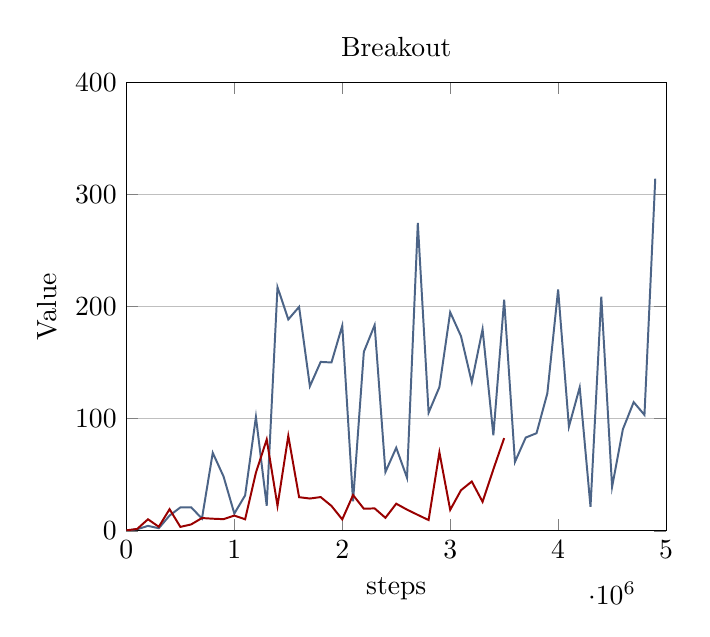
\begin{tikzpicture}

\begin{axis}[%
legend entries={rl-only-small-net,L2-reg,parallel-fs-50-no-aug}, 
legend columns=2,
title=Breakout,
legend to name=named,
legend style={legend cell align=left},
%%width=10in,
%%height=5in,
%%at={(2.596in,2.358in)},
% scale only axis,
xmin=0,
xmax=5000000,
xlabel style={font=\color{white!15!black}},
xlabel={steps},
xlabel near ticks,
ymin=0,
ymax=400,
ylabel style={font=\color{white!15!black}},
ylabel={Value},
ylabel near ticks,
ymajorgrids,
% %scale=0.5,
%%scale=0.4,
axis background/.style={fill=white},
%legend columns=2,
%legend=south outside
]
\addplot [color=blue, line width = 0.25mm]
                table[row sep=crcr]{
                  0 0.20000000298023224\\ 
100000 1.399999976158142\\ 
200000 4.400000095367432\\ 
300000 2.299999952316284\\ 
400000 13.600000381469727\\ 
500000 20.899999618530273\\ 
600000 21.0\\ 
700000 10.899999618530273\\ 
800000 69.5999984741211\\ 
900000 48.5\\ 
1000000 15.399999618530273\\ 
1100000 31.600000381469727\\ 
1200000 101.5999984741211\\ 
1300000 22.399999618530273\\ 
1400000 217.39999389648438\\ 
1500000 188.60000610351562\\ 
1600000 199.8000030517578\\ 
1700000 129.0\\ 
1800000 150.6999969482422\\ 
1900000 150.1999969482422\\ 
2000000 183.0\\ 
2100000 26.399999618530273\\ 
2200000 159.6999969482422\\ 
2300000 183.5\\ 
2400000 52.5\\ 
2500000 74.0999984741211\\ 
2600000 47.29999923706055\\ 
2700000 274.6000061035156\\ 
2800000 105.4000015258789\\ 
2900000 128.1999969482422\\ 
3000000 195.0\\ 
3100000 173.6999969482422\\ 
3200000 132.60000610351562\\ 
3300000 179.89999389648438\\ 
3400000 85.19999694824219\\ 
3500000 206.1999969482422\\ 
3600000 61.5\\ 
3700000 83.19999694824219\\ 
3800000 87.0999984741211\\ 
3900000 122.5999984741211\\ 
4000000 215.3000030517578\\ 
4100000 92.9000015258789\\ 
4200000 128.0\\ 
4300000 21.399999618530273\\ 
4400000 208.89999389648438\\ 
4500000 39.20000076293945\\ 
4600000 90.5999984741211\\ 
4700000 114.80000305175781\\ 
4800000 103.4000015258789\\ 
4900000 314.20001220703125\\ 
};
\addplot [color=red, line width = 0.25mm]
                table[row sep=crcr]{
                  0 0.4000000059604645\\ 
100000 1.7000000476837158\\ 
200000 10.300000190734863\\ 
300000 3.5999999046325684\\ 
400000 19.299999237060547\\ 
500000 3.5\\ 
600000 5.699999809265137\\ 
700000 11.399999618530273\\ 
800000 10.800000190734863\\ 
900000 10.399999618530273\\ 
1000000 13.600000381469727\\ 
1100000 10.300000190734863\\ 
1200000 51.900001525878906\\ 
1300000 81.5\\ 
1400000 22.299999237060547\\ 
1500000 84.69999694824219\\ 
1600000 30.0\\ 
1700000 28.799999237060547\\ 
1800000 30.100000381469727\\ 
1900000 22.200000762939453\\ 
2000000 10.199999809265137\\ 
2100000 31.899999618530273\\ 
2200000 19.700000762939453\\ 
2300000 20.0\\ 
2400000 11.600000381469727\\ 
2500000 24.200000762939453\\ 
2600000 18.899999618530273\\ 
2700000 14.199999809265137\\ 
2800000 9.600000381469727\\ 
2900000 70.0\\ 
3000000 18.700000762939453\\ 
3100000 36.20000076293945\\ 
3200000 44.0\\ 
3300000 25.899999618530273\\ 
3400000 54.900001525878906\\ 
3500000 82.69999694824219\\ 
};
\addplot [color=yellow, line width = 0.25mm]
                table[row sep=crcr]{
                  0 0.800000011920929\\ 
};
\end{axis}
\end{tikzpicture}}}
    \subfloat[]{  \resizebox{0.4\textwidth}{!}{
%\definecolor{blue}{RGB}{76,100,135}
%\definecolor{red}{RGB}{153,0,0}
%\definecolor{yellow}{RGB}{227,178,60}
%\definecolor{mycolor1}{rgb}{0.00000,0.44700,0.74100}%
%\definecolor{mycolor2}{rgb}{0.85000,0.32500,0.09800}%
%\definecolor{mycolor3}{rgb}{0.92900,0.69400,0.12500}%
%
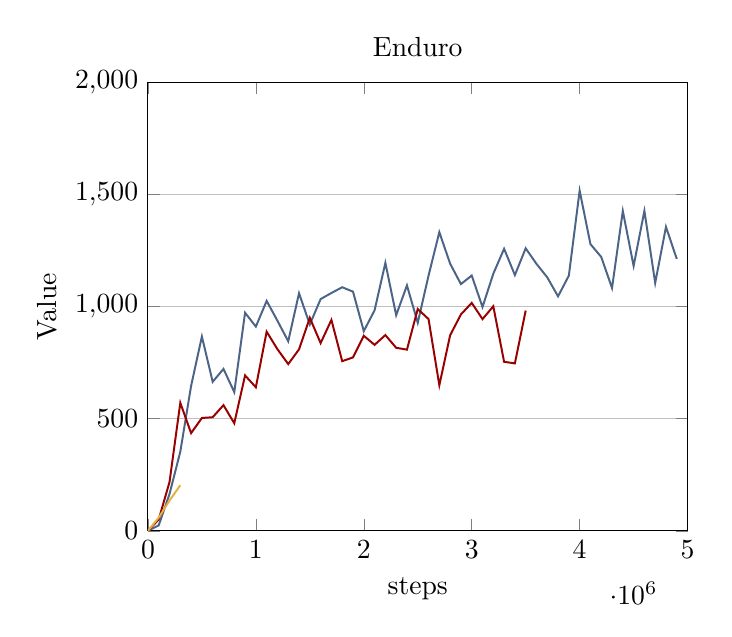
\begin{tikzpicture}

\begin{axis}[%
title=Enduro,
% %width=4.634in,
%%width=10in,
%%height=5in,
%at={(2.596in,2.358in)},
% scale only axis,
xmin=0,
xmax=5000000,
xlabel style={font=\color{white!15!black}},
xlabel={steps},
xlabel near ticks,
ymin=0,
ymax=2000,
ylabel style={font=\color{white!15!black}},
ylabel={Value},
ylabel near ticks,
ymajorgrids,
% %scale=0.5,
%scale=0.4,
axis background/.style={fill=white},
%legend style={legend cell align=left, align=left, draw=white!15!black}
]
\addplot [color=blue, line width = 0.25mm]
                table[row sep=crcr]{
                  0 0.0\\ 
100000 24.299999237060547\\ 
200000 164.3000030517578\\ 
300000 353.0\\ 
400000 646.4000244140625\\ 
500000 866.7000122070312\\ 
600000 664.7000122070312\\ 
700000 722.2000122070312\\ 
800000 618.9000244140625\\ 
900000 972.7999877929688\\ 
1000000 910.9000244140625\\ 
1100000 1025.699951171875\\ 
1200000 937.0\\ 
1300000 845.5999755859375\\ 
1400000 1059.9000244140625\\ 
1500000 920.2999877929688\\ 
1600000 1033.800048828125\\ 
1700000 1061.0\\ 
1800000 1086.5999755859375\\ 
1900000 1066.9000244140625\\ 
2000000 890.9000244140625\\ 
2100000 983.5\\ 
2200000 1195.300048828125\\ 
2300000 962.0\\ 
2400000 1094.800048828125\\ 
2500000 928.0\\ 
2600000 1138.5999755859375\\ 
2700000 1332.300048828125\\ 
2800000 1191.800048828125\\ 
2900000 1100.5999755859375\\ 
3000000 1138.800048828125\\ 
3100000 998.2999877929688\\ 
3200000 1146.800048828125\\ 
3300000 1258.0999755859375\\ 
3400000 1141.0\\ 
3500000 1260.300048828125\\ 
3600000 1190.800048828125\\ 
3700000 1130.5999755859375\\ 
3800000 1046.0999755859375\\ 
3900000 1138.4000244140625\\ 
4000000 1517.5\\ 
4100000 1278.9000244140625\\ 
4200000 1221.699951171875\\ 
4300000 1083.199951171875\\ 
4400000 1426.9000244140625\\ 
4500000 1181.5999755859375\\ 
4600000 1427.199951171875\\ 
4700000 1105.800048828125\\ 
4800000 1355.800048828125\\ 
4900000 1212.9000244140625\\ 
};
\addplot [color=red, line width = 0.25mm]
                table[row sep=crcr]{
                  0 0.0\\ 
100000 50.5\\ 
200000 217.60000610351562\\ 
300000 570.9000244140625\\ 
400000 435.6000061035156\\ 
500000 503.3999938964844\\ 
600000 506.79998779296875\\ 
700000 560.5\\ 
800000 479.79998779296875\\ 
900000 693.2000122070312\\ 
1000000 640.4000244140625\\ 
1100000 888.4000244140625\\ 
1200000 810.0999755859375\\ 
1300000 743.7999877929688\\ 
1400000 809.5\\ 
1500000 950.2000122070312\\ 
1600000 837.4000244140625\\ 
1700000 940.7999877929688\\ 
1800000 756.7999877929688\\ 
1900000 773.5\\ 
2000000 870.0999755859375\\ 
2100000 829.5999755859375\\ 
2200000 873.2000122070312\\ 
2300000 816.5\\ 
2400000 808.2000122070312\\ 
2500000 989.5999755859375\\ 
2600000 944.5\\ 
2700000 649.4000244140625\\ 
2800000 872.4000244140625\\ 
2900000 965.2000122070312\\ 
3000000 1016.7000122070312\\ 
3100000 944.4000244140625\\ 
3200000 1001.7000122070312\\ 
3300000 754.0\\ 
3400000 746.7999877929688\\ 
3500000 982.2999877929688\\ 
};
\addplot [color=yellow, line width = 0.25mm]
                table[row sep=crcr]{
                  0 0.0\\ 
100000 58.79999923706055\\ 
200000 135.10000610351562\\ 
300000 203.1999969482422\\ 
};
\end{axis}
\end{tikzpicture}}}\\
  \vspace{-1cm}
    \subfloat[]{  \resizebox{0.4\textwidth}{!}{
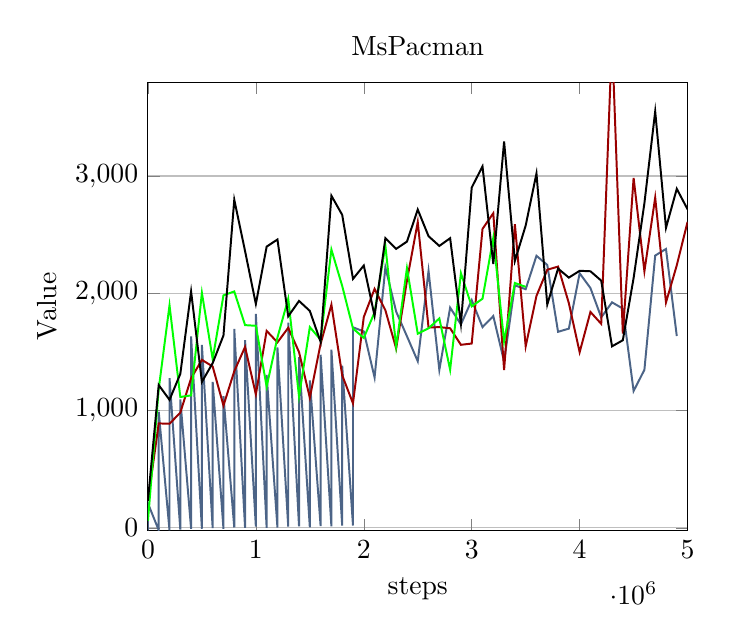
\begin{tikzpicture}

\begin{axis}[%
title=MsPacman,
% %width=4.634in,
%width=10in,
%height=5in,
%at={(2.596in,2.358in)},
% scale only axis,
xmin=0,
xmax=5000000,
xlabel style={font=\color{white!15!black}},
xlabel={steps},
xlabel near ticks,
ymin=-22,
ymax=3800,
ylabel style={font=\color{white!15!black}},
ylabel={Value},
ylabel near ticks,
ymajorgrids,
% %scale=0.5,
%scale=0.4,
axis background/.style={fill=white},
%legend style={legend cell align=left, align=left, draw=white!15!black}
]
\addplot [color=blue, line width = 0.25mm]
                table[row sep=crcr]{
                  0 -21.0\\ 
0 210.0\\ 
100000 -19.799999237060547\\ 
100000 990.0\\ 
200000 -20.700000762939453\\ 
200000 1277.0\\ 
300000 -15.0\\ 
300000 1096.0\\ 
400000 -7.0\\ 
400000 1632.0\\ 
500000 -6.900000095367432\\ 
500000 1561.0\\ 
600000 -1.899999976158142\\ 
600000 1245.0\\ 
700000 -7.599999904632568\\ 
700000 1123.0\\ 
800000 4.0\\ 
800000 1696.0\\ 
900000 1.5\\ 
900000 1600.0\\ 
1000000 11.300000190734863\\ 
1000000 1824.0\\ 
1100000 1.2000000476837158\\ 
1100000 1304.0\\ 
1200000 3.700000047683716\\ 
1200000 1538.0\\ 
1300000 11.5\\ 
1300000 1750.0\\ 
1400000 13.600000381469727\\ 
1400000 1456.0\\ 
1500000 5.699999809265137\\ 
1500000 1258.0\\ 
1600000 15.600000381469727\\ 
1600000 1476.0\\ 
1700000 13.5\\ 
1700000 1519.0\\ 
1800000 19.299999237060547\\ 
1800000 1383.0\\ 
1900000 20.799999237060547\\ 
1900000 1710.0\\ 
2000000 1675.0\\ 
2100000 1282.0\\ 
2200000 2222.0\\ 
2300000 1844.0\\ 
2400000 1634.0\\ 
2500000 1421.0\\ 
2600000 2191.0\\ 
2700000 1347.0\\ 
2800000 1878.0\\ 
2900000 1735.0\\ 
3000000 1942.0\\ 
3100000 1712.0\\ 
3200000 1806.0\\ 
3300000 1419.0\\ 
3400000 2068.0\\ 
3500000 2035.0\\ 
3600000 2320.0\\ 
3700000 2242.0\\ 
3800000 1672.0\\ 
3900000 1699.0\\ 
4000000 2171.0\\ 
4100000 2045.0\\ 
4200000 1795.0\\ 
4300000 1923.0\\ 
4400000 1870.0\\ 
4500000 1167.0\\ 
4600000 1348.0\\ 
4700000 2322.0\\ 
4800000 2378.0\\ 
4900000 1636.0\\ 
};
\addplot [color=red, line width = 0.25mm]
                table[row sep=crcr]{
                  0 230.0\\ 
100000 891.0\\ 
200000 888.0\\ 
300000 983.0\\ 
400000 1276.0\\ 
500000 1433.0\\ 
600000 1376.0\\ 
700000 1043.0\\ 
800000 1336.0\\ 
900000 1543.0\\ 
1000000 1139.0\\ 
1100000 1680.0\\ 
1200000 1582.0\\ 
1300000 1706.0\\ 
1400000 1499.0\\ 
1500000 1110.0\\ 
1600000 1569.0\\ 
1700000 1903.0\\ 
1800000 1301.0\\ 
1900000 1062.0\\ 
2000000 1798.0\\ 
2100000 2038.0\\ 
2200000 1856.0\\ 
2300000 1530.0\\ 
2400000 2109.0\\ 
2500000 2607.0\\ 
2600000 1708.0\\ 
2700000 1712.0\\ 
2800000 1702.0\\ 
2900000 1561.0\\ 
3000000 1572.0\\ 
3100000 2549.0\\ 
3200000 2683.0\\ 
3300000 1346.0\\ 
3400000 2590.0\\ 
3500000 1548.0\\ 
3600000 1978.0\\ 
3700000 2201.0\\ 
3800000 2228.0\\ 
3900000 1916.0\\ 
4000000 1498.0\\ 
4100000 1841.0\\ 
4200000 1740.0\\ 
4300000 4177.0\\ 
4400000 1656.0\\ 
4500000 2984.0\\ 
4600000 2188.0\\ 
4700000 2816.0\\ 
4800000 1922.0\\ 
4900000 2239.0\\ 
5000000 2609.0\\ 
};
\addplot [color=green, line width = 0.25mm]
                table[row sep=crcr]{
                  0 60.0\\ 
100000 1185.0\\ 
200000 1898.0\\ 
300000 1116.0\\ 
400000 1130.0\\ 
500000 2004.0\\ 
600000 1439.0\\ 
700000 1983.0\\ 
800000 2016.0\\ 
900000 1729.0\\ 
1000000 1723.0\\ 
1100000 1205.0\\ 
1200000 1623.0\\ 
1300000 1954.0\\ 
1400000 1121.0\\ 
1500000 1712.0\\ 
1600000 1604.0\\ 
1700000 2373.0\\ 
1800000 2063.0\\ 
1900000 1700.0\\ 
2000000 1620.0\\ 
2100000 1838.0\\ 
2200000 2406.0\\ 
2300000 1546.0\\ 
2400000 2215.0\\ 
2500000 1656.0\\ 
2600000 1702.0\\ 
2700000 1786.0\\ 
2800000 1348.0\\ 
2900000 2172.0\\ 
3000000 1889.0\\ 
3100000 1954.0\\ 
3200000 2473.0\\ 
3300000 1591.0\\ 
3400000 2088.0\\ 
3500000 2055.0\\ 
};
\addplot [color=black, line width = 0.25mm]
                table[row sep=crcr]{
                  0 230.0\\ 
100000 1218.0\\ 
200000 1092.0\\ 
300000 1313.0\\ 
400000 2016.0\\ 
500000 1245.0\\ 
600000 1405.0\\ 
700000 1641.0\\ 
800000 2798.0\\ 
900000 2360.0\\ 
1000000 1909.0\\ 
1100000 2398.0\\ 
1200000 2459.0\\ 
1300000 1804.0\\ 
1400000 1935.0\\ 
1500000 1850.0\\ 
1600000 1586.0\\ 
1700000 2832.0\\ 
1800000 2669.0\\ 
1900000 2123.0\\ 
2000000 2237.0\\ 
2100000 1808.0\\ 
2200000 2470.0\\ 
2300000 2379.0\\ 
2400000 2441.0\\ 
2500000 2714.0\\ 
2600000 2487.0\\ 
2700000 2404.0\\ 
2800000 2470.0\\ 
2900000 1739.0\\ 
3000000 2902.0\\ 
3100000 3082.0\\ 
3200000 2250.0\\ 
3300000 3294.0\\ 
3400000 2276.0\\ 
3500000 2578.0\\ 
3600000 3022.0\\ 
3700000 1904.0\\ 
3800000 2211.0\\ 
3900000 2134.0\\ 
4000000 2192.0\\ 
4100000 2188.0\\ 
4200000 2108.0\\ 
4300000 1548.0\\ 
4400000 1600.0\\ 
4500000 2130.0\\ 
4600000 2768.0\\ 
4700000 3551.0\\ 
4800000 2558.0\\ 
4900000 2891.0\\ 
5000000 2716.0\\ 
};
\end{axis}
\end{tikzpicture}}}
    \subfloat[]{  \resizebox{0.4\textwidth}{!}{
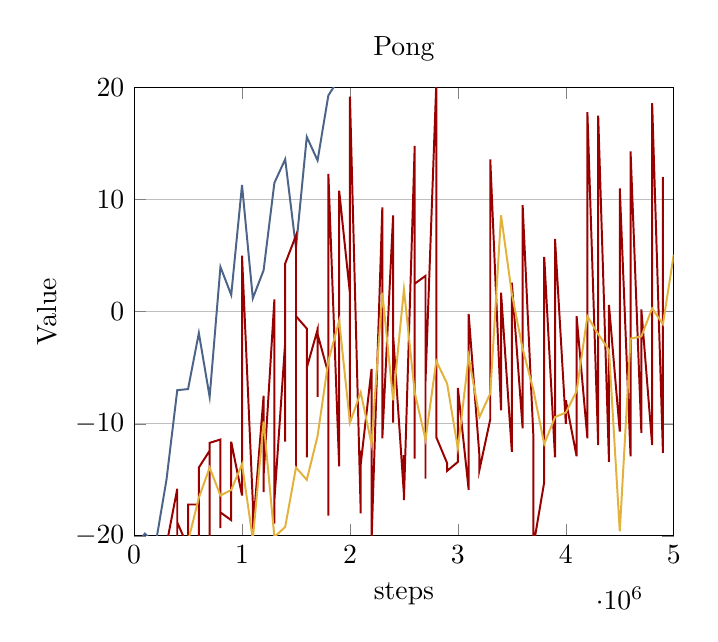
\begin{tikzpicture}

\begin{axis}[%
title=Pong,
% %width=4.634in,
%width=10in,
%height=5in,
%at={(2.596in,2.358in)},
% scale only axis,
xmin=0,
xmax=5000000,
xlabel style={font=\color{white!15!black}},
xlabel={steps},
xlabel near ticks,
ymin=-20,
ymax=20,
ylabel style={font=\color{white!15!black}},
ylabel={Value},
ylabel near ticks,
ymajorgrids,
% %scale=0.5,
%scale=0.4,
axis background/.style={fill=white},
%legend style={legend cell align=left, align=left, draw=white!15!black}
]
\addplot [color=blue, line width = 0.25mm]
                table[row sep=crcr]{
                  0 -21.0\\ 
100000 -19.799999237060547\\ 
200000 -20.700000762939453\\ 
300000 -15.0\\ 
400000 -7.0\\ 
500000 -6.900000095367432\\ 
600000 -1.899999976158142\\ 
700000 -7.599999904632568\\ 
800000 4.0\\ 
900000 1.5\\ 
1000000 11.300000190734863\\ 
1100000 1.2000000476837158\\ 
1200000 3.700000047683716\\ 
1300000 11.5\\ 
1400000 13.600000381469727\\ 
1500000 5.699999809265137\\ 
1600000 15.600000381469727\\ 
1700000 13.5\\ 
1800000 19.299999237060547\\ 
1900000 20.799999237060547\\ 
};
\addplot [color=red, line width = 0.25mm]
                table[row sep=crcr]{
                  0 -21.0\\ 
0 -21.0\\ 
0 -21.0\\ 
0 -21.0\\ 
100000 -21.0\\ 
100000 -20.600000381469727\\ 
100000 -21.0\\ 
200000 -20.399999618530273\\ 
200000 -21.0\\ 
200000 -20.799999237060547\\ 
300000 -20.600000381469727\\ 
300000 -20.799999237060547\\ 
300000 -20.799999237060547\\ 
400000 -15.800000190734863\\ 
400000 -20.399999618530273\\ 
400000 -18.799999237060547\\ 
500000 -21.0\\ 
500000 -21.0\\ 
500000 -17.200000762939453\\ 
600000 -17.200000762939453\\ 
600000 -20.600000381469727\\ 
600000 -13.899999618530273\\ 
700000 -12.399999618530273\\ 
700000 -20.100000381469727\\ 
700000 -11.699999809265137\\ 
800000 -11.399999618530273\\ 
800000 -19.299999237060547\\ 
800000 -17.899999618530273\\ 
900000 -18.600000381469727\\ 
900000 -15.699999809265137\\ 
900000 -11.600000381469727\\ 
1000000 -16.399999618530273\\ 
1000000 -16.0\\ 
1000000 5.0\\ 
1100000 -17.0\\ 
1100000 -17.5\\ 
1100000 -19.600000381469727\\ 
1200000 -7.5\\ 
1200000 -16.100000381469727\\ 
1200000 -14.600000381469727\\ 
1300000 1.100000023841858\\ 
1300000 -18.899999618530273\\ 
1300000 -16.799999237060547\\ 
1400000 -2.700000047683716\\ 
1400000 -11.600000381469727\\ 
1400000 4.300000190734863\\ 
1500000 6.800000190734863\\ 
1500000 -13.899999618530273\\ 
1500000 -0.4000000059604645\\ 
1600000 -1.5\\ 
1600000 -13.0\\ 
1600000 -5.0\\ 
1700000 -1.600000023841858\\ 
1700000 -7.599999904632568\\ 
1700000 -2.0\\ 
1800000 -5.5\\ 
1800000 -18.200000762939453\\ 
1800000 12.300000190734863\\ 
1900000 -13.800000190734863\\ 
1900000 -10.0\\ 
1900000 10.800000190734863\\ 
2000000 1.600000023841858\\ 
2000000 -9.899999618530273\\ 
2000000 19.200000762939453\\ 
2100000 -18.0\\ 
2100000 -12.399999618530273\\ 
2100000 -13.600000381469727\\ 
2200000 -5.099999904632568\\ 
2200000 -13.899999618530273\\ 
2200000 -20.5\\ 
2300000 9.300000190734863\\ 
2300000 -8.199999809265137\\ 
2300000 -11.300000190734863\\ 
2400000 8.600000381469727\\ 
2400000 -9.899999618530273\\ 
2400000 -2.0999999046325684\\ 
2500000 -16.299999237060547\\ 
2500000 -12.800000190734863\\ 
2500000 -16.799999237060547\\ 
2600000 14.800000190734863\\ 
2600000 -13.100000381469727\\ 
2600000 2.5\\ 
2700000 3.200000047683716\\ 
2700000 -14.899999618530273\\ 
2700000 -6.199999809265137\\ 
2800000 20.399999618530273\\ 
2800000 -9.800000190734863\\ 
2800000 -11.199999809265137\\ 
2900000 -13.5\\ 
2900000 -14.199999809265137\\ 
3000000 -13.399999618530273\\ 
3000000 -6.800000190734863\\ 
3100000 -15.899999618530273\\ 
3100000 -0.20000000298023224\\ 
3200000 -12.899999618530273\\ 
3200000 -14.100000381469727\\ 
3300000 -9.600000381469727\\ 
3300000 13.600000381469727\\ 
3400000 -8.800000190734863\\ 
3400000 1.7000000476837158\\ 
3500000 -12.5\\ 
3500000 2.5999999046325684\\ 
3600000 -10.399999618530273\\ 
3600000 9.5\\ 
3700000 -11.199999809265137\\ 
3700000 -20.899999618530273\\ 
3800000 -15.199999809265137\\ 
3800000 4.900000095367432\\ 
3900000 -13.0\\ 
3900000 6.5\\ 
4000000 -10.0\\ 
4000000 -7.900000095367432\\ 
4100000 -12.899999618530273\\ 
4100000 -0.4000000059604645\\ 
4200000 -11.300000190734863\\ 
4200000 17.799999237060547\\ 
4300000 -11.899999618530273\\ 
4300000 17.5\\ 
4400000 -13.399999618530273\\ 
4400000 0.6000000238418579\\ 
4500000 -10.699999809265137\\ 
4500000 11.0\\ 
4600000 -12.899999618530273\\ 
4600000 14.300000190734863\\ 
4700000 -10.800000190734863\\ 
4700000 0.20000000298023224\\ 
4800000 -11.899999618530273\\ 
4800000 18.600000381469727\\ 
4900000 -12.600000381469727\\ 
4900000 12.0\\ 
};
\addplot [color=yellow, line width = 0.25mm]
                table[row sep=crcr]{
                  0 -21.0\\ 
0 -21.0\\ 
100000 -21.0\\ 
200000 -21.0\\ 
300000 -20.399999618530273\\ 
400000 -21.0\\ 
500000 -20.5\\ 
600000 -16.600000381469727\\ 
700000 -13.899999618530273\\ 
800000 -16.399999618530273\\ 
900000 -15.899999618530273\\ 
1000000 -13.600000381469727\\ 
1100000 -20.299999237060547\\ 
1200000 -9.800000190734863\\ 
1300000 -20.100000381469727\\ 
1400000 -19.200000762939453\\ 
1500000 -13.899999618530273\\ 
1600000 -15.0\\ 
1700000 -11.100000381469727\\ 
1800000 -4.400000095367432\\ 
1900000 -0.800000011920929\\ 
2000000 -9.899999618530273\\ 
2100000 -7.199999809265137\\ 
2200000 -11.800000190734863\\ 
2300000 1.7000000476837158\\ 
2400000 -7.900000095367432\\ 
2500000 2.0\\ 
2600000 -7.199999809265137\\ 
2700000 -11.399999618530273\\ 
2800000 -4.400000095367432\\ 
2900000 -6.400000095367432\\ 
3000000 -12.199999809265137\\ 
3100000 -4.0\\ 
3200000 -9.399999618530273\\ 
3300000 -7.300000190734863\\ 
3400000 8.600000381469727\\ 
3500000 1.600000023841858\\ 
3600000 -3.299999952316284\\ 
3700000 -7.0\\ 
3800000 -11.800000190734863\\ 
3900000 -9.399999618530273\\ 
4000000 -9.0\\ 
4100000 -7.099999904632568\\ 
4200000 -0.4000000059604645\\ 
4300000 -2.0\\ 
4400000 -3.4000000953674316\\ 
4500000 -19.600000381469727\\ 
4600000 -2.4000000953674316\\ 
4700000 -2.200000047683716\\ 
4800000 0.30000001192092896\\ 
4900000 -1.100000023841858\\ 
5000000 5.099999904632568\\ 
};
\end{axis}
\end{tikzpicture}}}\\
  \vspace{-1cm}
    \subfloat[]{  \resizebox{0.4\textwidth}{!}{
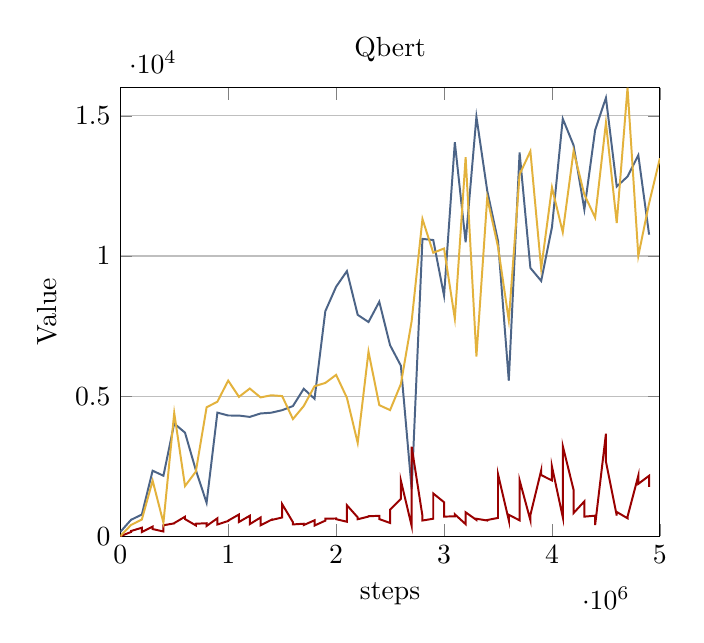
\begin{tikzpicture}

\begin{axis}[%
title=Qbert,
% %width=4.634in,
%width=10in,
%height=5in,
%at={(2.596in,2.358in)},
% scale only axis,
xmin=0,
xmax=5000000,
xlabel style={font=\color{white!15!black}},
xlabel={steps},
xlabel near ticks,
ymin=0,
ymax=16000,
ylabel style={font=\color{white!15!black}},
ylabel={Value},
ylabel near ticks,
ymajorgrids,
% %scale=0.5,
%scale=0.4,
axis background/.style={fill=white},
%legend style={legend cell align=left, align=left, draw=white!15!black}
]
\addplot [color=blue, line width = 0.25mm]
                table[row sep=crcr]{
                  0 150.0\\ 
100000 585.0\\ 
200000 772.5\\ 
300000 2337.5\\ 
400000 2157.5\\ 
500000 4022.5\\ 
600000 3695.0\\ 
700000 2362.5\\ 
800000 1192.5\\ 
900000 4410.0\\ 
1000000 4307.5\\ 
1100000 4305.0\\ 
1200000 4257.5\\ 
1300000 4380.0\\ 
1400000 4407.5\\ 
1500000 4497.5\\ 
1600000 4645.0\\ 
1700000 5260.0\\ 
1800000 4905.0\\ 
1900000 8030.0\\ 
2000000 8902.5\\ 
2100000 9460.0\\ 
2200000 7900.0\\ 
2300000 7642.5\\ 
2400000 8367.5\\ 
2500000 6815.0\\ 
2600000 6085.0\\ 
2700000 1677.5\\ 
2800000 10610.0\\ 
2900000 10570.0\\ 
3000000 8585.0\\ 
3100000 14057.5\\ 
3200000 10490.0\\ 
3300000 14970.0\\ 
3400000 12332.5\\ 
3500000 10537.5\\ 
3600000 5550.0\\ 
3700000 13692.5\\ 
3800000 9572.5\\ 
3900000 9110.0\\ 
4000000 11030.0\\ 
4100000 14897.5\\ 
4200000 13955.0\\ 
4300000 11660.0\\ 
4400000 14495.0\\ 
4500000 15645.0\\ 
4600000 12480.0\\ 
4700000 12835.0\\ 
4800000 13597.5\\ 
4900000 10762.5\\ 
};
\addplot [color=red, line width = 0.25mm]
                table[row sep=crcr]{
                  0 0.0\\ 
0 0.0\\ 
100000 150.0\\ 
100000 185.0\\ 
200000 302.5\\ 
200000 150.0\\ 
300000 342.5\\ 
300000 255.0\\ 
400000 167.5\\ 
400000 390.0\\ 
500000 457.5\\ 
500000 467.5\\ 
600000 695.0\\ 
600000 610.0\\ 
700000 385.0\\ 
700000 445.0\\ 
800000 462.5\\ 
800000 365.0\\ 
900000 640.0\\ 
900000 417.5\\ 
1000000 542.5\\ 
1000000 555.0\\ 
1100000 775.0\\ 
1100000 507.5\\ 
1200000 730.0\\ 
1200000 430.0\\ 
1300000 667.5\\ 
1300000 387.5\\ 
1400000 585.0\\ 
1400000 577.5\\ 
1500000 667.5\\ 
1500000 1145.0\\ 
1600000 500.0\\ 
1600000 420.0\\ 
1700000 445.0\\ 
1700000 397.5\\ 
1800000 567.5\\ 
1800000 380.0\\ 
1900000 555.0\\ 
1900000 625.0\\ 
2000000 632.5\\ 
2000000 607.5\\ 
2100000 515.0\\ 
2100000 1105.0\\ 
2200000 672.5\\ 
2200000 605.0\\ 
2300000 700.0\\ 
2300000 712.5\\ 
2400000 727.5\\ 
2400000 610.0\\ 
2500000 472.5\\ 
2500000 947.5\\ 
2600000 1330.0\\ 
2600000 1985.0\\ 
2700000 365.0\\ 
2700000 3195.0\\ 
2800000 720.0\\ 
2800000 560.0\\ 
2900000 622.5\\ 
2900000 1525.0\\ 
3000000 1212.5\\ 
3000000 700.0\\ 
3100000 707.5\\ 
3100000 780.0\\ 
3200000 430.0\\ 
3200000 852.5\\ 
3300000 580.0\\ 
3300000 622.5\\ 
3400000 560.0\\ 
3400000 577.5\\ 
3500000 652.5\\ 
3500000 2215.0\\ 
3600000 567.5\\ 
3600000 765.0\\ 
3700000 565.0\\ 
3700000 1995.0\\ 
3800000 570.0\\ 
3800000 757.5\\ 
3900000 2345.0\\ 
3900000 2182.5\\ 
4000000 1987.5\\ 
4000000 2482.5\\ 
4100000 682.5\\ 
4100000 3220.0\\ 
4200000 1657.5\\ 
4200000 825.0\\ 
4300000 1242.5\\ 
4300000 697.5\\ 
4400000 732.5\\ 
4400000 397.5\\ 
4500000 3660.0\\ 
4500000 2662.5\\ 
4600000 735.0\\ 
4600000 865.0\\ 
4700000 640.0\\ 
4700000 695.0\\ 
4800000 2160.0\\ 
4800000 1867.5\\ 
4900000 2157.5\\ 
4900000 1762.5\\ 
};
\addplot [color=yellow, line width = 0.25mm]
                table[row sep=crcr]{
                  0 0.0\\ 
0 0.0\\ 
0 0.0\\ 
0 0.0\\ 
100000 400.0\\ 
200000 595.0\\ 
300000 1982.5\\ 
400000 480.0\\ 
500000 4397.5\\ 
600000 1790.0\\ 
700000 2302.5\\ 
800000 4600.0\\ 
900000 4800.0\\ 
1000000 5552.5\\ 
1100000 4972.5\\ 
1200000 5270.0\\ 
1300000 4952.5\\ 
1400000 5030.0\\ 
1500000 5000.0\\ 
1600000 4180.0\\ 
1700000 4645.0\\ 
1800000 5352.5\\ 
1900000 5470.0\\ 
2000000 5757.5\\ 
2100000 4940.0\\ 
2200000 3327.5\\ 
2300000 6585.0\\ 
2400000 4677.5\\ 
2500000 4500.0\\ 
2600000 5430.0\\ 
2700000 7677.5\\ 
2800000 11320.0\\ 
2900000 10115.0\\ 
3000000 10267.5\\ 
3100000 7765.0\\ 
3200000 13525.0\\ 
3300000 6415.0\\ 
3400000 12077.5\\ 
3500000 10327.5\\ 
3600000 7700.0\\ 
3700000 12912.5\\ 
3800000 13737.5\\ 
3900000 9552.5\\ 
4000000 12445.0\\ 
4100000 10847.5\\ 
4200000 13737.5\\ 
4300000 12195.0\\ 
4400000 11370.0\\ 
4500000 14755.0\\ 
4600000 11175.0\\ 
4700000 16002.5\\ 
4800000 10005.0\\ 
4900000 11885.0\\ 
5000000 13490.0\\ 
};
\end{axis}
\end{tikzpicture}}}
    \subfloat[]{  \resizebox{0.4\textwidth}{!}{
\definecolor{blue}{RGB}{76,100,135}
\definecolor{red}{RGB}{153,0,0}
\definecolor{yellow}{RGB}{227,178,60}
\definecolor{mycolor1}{rgb}{0.00000,0.44700,0.74100}%
\definecolor{mycolor2}{rgb}{0.85000,0.32500,0.09800}%
\definecolor{mycolor3}{rgb}{0.92900,0.69400,0.12500}%
%
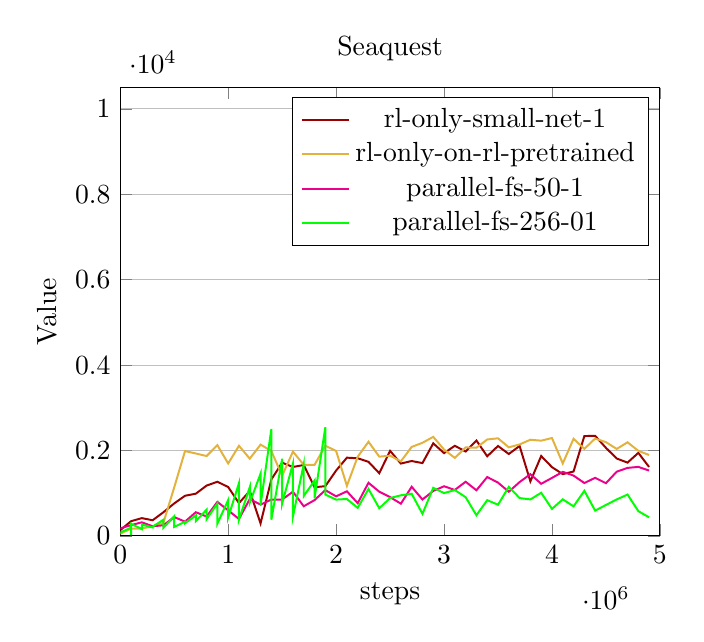
\begin{tikzpicture}

\begin{axis}[%
title=Seaquest,
% %width=4.634in,
%width=10in,
%height=5in,
%at={(2.596in,2.358in)},
% scale only axis,
xmin=0,
xmax=5000000,
xlabel style={font=\color{white!15!black}},
xlabel={steps},
xlabel near ticks,
ymin=0,
ymax=10500,
ylabel style={font=\color{white!15!black}},
ylabel={Value},
ylabel near ticks,
ymajorgrids,
% %scale=0.5,
%scale=0.4,
axis background/.style={fill=white},
%legend style={legend cell align=left, align=left, draw=white!15!black}
]
\addplot [color=red, line width = 0.25mm]
                table[row sep=crcr]{
                  0 134.0\\ 
100000 344.0\\ 
200000 416.0\\ 
300000 366.0\\ 
400000 554.0\\ 
500000 760.0\\ 
600000 940.0\\ 
700000 988.0\\ 
800000 1178.0\\ 
900000 1268.0\\ 
1000000 1144.0\\ 
1100000 768.0\\ 
1200000 1052.0\\ 
1300000 292.0\\ 
1400000 1322.0\\ 
1500000 1714.0\\ 
1600000 1614.0\\ 
1700000 1660.0\\ 
1800000 1140.0\\ 
1900000 1164.0\\ 
2000000 1530.0\\ 
2100000 1832.0\\ 
2200000 1818.0\\ 
2300000 1734.0\\ 
2400000 1468.0\\ 
2500000 1992.0\\ 
2600000 1694.0\\ 
2700000 1754.0\\ 
2800000 1704.0\\ 
2900000 2168.0\\ 
3000000 1938.0\\ 
3100000 2110.0\\ 
3200000 1976.0\\ 
3300000 2234.0\\ 
3400000 1864.0\\ 
3500000 2106.0\\ 
3600000 1918.0\\ 
3700000 2106.0\\ 
3800000 1276.0\\ 
3900000 1870.0\\ 
4000000 1610.0\\ 
4100000 1446.0\\ 
4200000 1508.0\\ 
4300000 2338.0\\ 
4400000 2344.0\\ 
4500000 2062.0\\ 
4600000 1812.0\\ 
4700000 1716.0\\ 
4800000 1944.0\\ 
4900000 1614.0\\ 
};
\addlegendentry{rl-only-small-net-1}
\addplot [color=yellow, line width = 0.25mm]
                table[row sep=crcr]{
                  0 48.0\\ 
100000 172.0\\ 
200000 172.0\\ 
300000 224.0\\ 
400000 308.0\\ 
500000 1136.0\\ 
600000 1986.0\\ 
700000 1930.0\\ 
800000 1870.0\\ 
900000 2124.0\\ 
1000000 1696.0\\ 
1100000 2110.0\\ 
1200000 1808.0\\ 
1300000 2138.0\\ 
1400000 1988.0\\ 
1500000 1408.0\\ 
1600000 1974.0\\ 
1700000 1664.0\\ 
1800000 1662.0\\ 
1900000 2112.0\\ 
2000000 1990.0\\ 
2100000 1172.0\\ 
2200000 1854.0\\ 
2300000 2204.0\\ 
2400000 1856.0\\ 
2500000 1878.0\\ 
2600000 1746.0\\ 
2700000 2084.0\\ 
2800000 2180.0\\ 
2900000 2320.0\\ 
3000000 2022.0\\ 
3100000 1826.0\\ 
3200000 2072.0\\ 
3300000 2064.0\\ 
3400000 2258.0\\ 
3500000 2286.0\\ 
3600000 2074.0\\ 
3700000 2142.0\\ 
3800000 2252.0\\ 
3900000 2230.0\\ 
4000000 2292.0\\ 
4100000 1696.0\\ 
4200000 2274.0\\ 
4300000 2038.0\\ 
4400000 2280.0\\ 
4500000 2196.0\\ 
4600000 2036.0\\ 
4700000 2192.0\\ 
4800000 1992.0\\ 
4900000 1894.0\\ 
};
\addlegendentry{rl-only-on-rl-pretrained}
\addplot [color=magenta, line width = 0.25mm]
                table[row sep=crcr]{
                  0 176.0\\ 
0 176.0\\ 
100000 252.0\\ 
200000 318.0\\ 
300000 226.0\\ 
400000 248.0\\ 
500000 440.0\\ 
600000 334.0\\ 
700000 554.0\\ 
800000 454.0\\ 
900000 796.0\\ 
1000000 598.0\\ 
1100000 396.0\\ 
1200000 862.0\\ 
1300000 732.0\\ 
1400000 850.0\\ 
1500000 852.0\\ 
1600000 1034.0\\ 
1700000 694.0\\ 
1800000 838.0\\ 
1900000 1072.0\\ 
2000000 926.0\\ 
2100000 1044.0\\ 
2200000 766.0\\ 
2300000 1244.0\\ 
2400000 1034.0\\ 
2500000 908.0\\ 
2600000 754.0\\ 
2700000 1150.0\\ 
2800000 852.0\\ 
2900000 1052.0\\ 
3000000 1162.0\\ 
3100000 1076.0\\ 
3200000 1268.0\\ 
3300000 1068.0\\ 
3400000 1378.0\\ 
3500000 1248.0\\ 
3600000 1034.0\\ 
3700000 1260.0\\ 
3800000 1446.0\\ 
3900000 1220.0\\ 
4000000 1358.0\\ 
4100000 1500.0\\ 
4200000 1412.0\\ 
4300000 1238.0\\ 
4400000 1360.0\\ 
4500000 1234.0\\ 
4600000 1504.0\\ 
4700000 1592.0\\ 
4800000 1616.0\\ 
4900000 1530.0\\ 
};
\addlegendentry{parallel-fs-50-1}
\addplot [color=green, line width = 0.25mm]
                table[row sep=crcr]{
                  0 80.0\\ 
0 80.0\\ 
0 80.0\\ 
100000 192.0\\ 
100000 20.0\\ 
100000 284.0\\ 
200000 158.0\\ 
200000 264.0\\ 
300000 198.0\\ 
300000 216.0\\ 
400000 378.0\\ 
400000 192.0\\ 
500000 460.0\\ 
500000 210.0\\ 
600000 330.0\\ 
600000 296.0\\ 
700000 478.0\\ 
700000 344.0\\ 
800000 614.0\\ 
800000 390.0\\ 
900000 758.0\\ 
900000 288.0\\ 
1000000 840.0\\ 
1000000 432.0\\ 
1100000 1236.0\\ 
1100000 384.0\\ 
1200000 1142.0\\ 
1200000 776.0\\ 
1300000 1458.0\\ 
1300000 730.0\\ 
1400000 2504.0\\ 
1400000 380.0\\ 
1500000 1806.0\\ 
1500000 756.0\\ 
1600000 1695.0\\ 
1600000 454.0\\ 
1700000 1678.0\\ 
1700000 932.0\\ 
1800000 1296.0\\ 
1800000 878.0\\ 
1900000 2544.0\\ 
1900000 968.0\\ 
2000000 850.0\\ 
2100000 864.0\\ 
2200000 656.0\\ 
2300000 1098.0\\ 
2400000 648.0\\ 
2500000 886.0\\ 
2600000 950.0\\ 
2700000 988.0\\ 
2800000 516.0\\ 
2900000 1126.0\\ 
3000000 1002.0\\ 
3100000 1074.0\\ 
3200000 906.0\\ 
3300000 484.0\\ 
3400000 836.0\\ 
3500000 730.0\\ 
3600000 1148.0\\ 
3700000 886.0\\ 
3800000 854.0\\ 
3900000 1010.0\\ 
4000000 632.0\\ 
4100000 856.0\\ 
4200000 692.0\\ 
4300000 1056.0\\ 
4400000 592.0\\ 
4500000 724.0\\ 
4600000 854.0\\ 
4700000 968.0\\ 
4800000 580.0\\ 
4900000 434.0\\ 
};
\addlegendentry{parallel-fs-256-01}
\end{axis}
\end{tikzpicture}}}\\
  \vspace{-1cm}
    \subfloat[]{  \resizebox{0.4\textwidth}{!}{
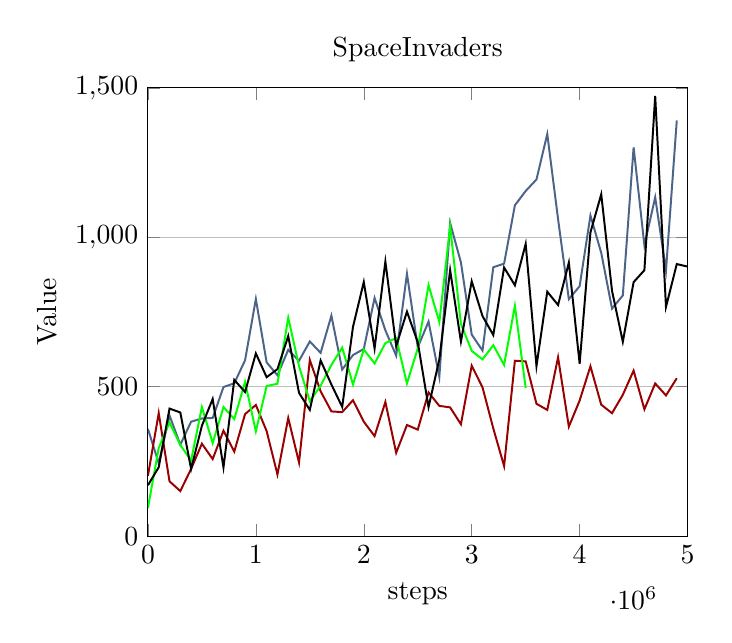
\begin{tikzpicture}

\begin{axis}[%
title=SpaceInvaders,
%width=10in,
%height=5in,
%at={(2.596in,2.358in)},
% scale only axis,
xmin=0,
xmax=5000000,
xlabel style={font=\color{white!15!black}},
xlabel={steps},
xlabel near ticks,
ymin=0,
ymax=1500,
ylabel style={font=\color{white!15!black}},
ylabel={Value},
ylabel near ticks,
ymajorgrids,
% %scale=0.5,
%scale=0.4,
axis background/.style={fill=white},
%legend style={legend cell align=left, align=left, draw=white!15!black}
]
\addplot [color=blue, line width = 0.25mm]
                table[row sep=crcr]{
                  0 359.0\\ 
100000 244.0\\ 
200000 404.0\\ 
300000 306.0\\ 
400000 383.0\\ 
500000 394.0\\ 
600000 395.5\\ 
700000 499.0\\ 
800000 511.5\\ 
900000 588.5\\ 
1000000 793.5\\ 
1100000 581.5\\ 
1200000 538.5\\ 
1300000 623.5\\ 
1400000 587.0\\ 
1500000 651.5\\ 
1600000 613.5\\ 
1700000 738.0\\ 
1800000 557.5\\ 
1900000 606.0\\ 
2000000 626.5\\ 
2100000 797.0\\ 
2200000 689.0\\ 
2300000 604.0\\ 
2400000 878.0\\ 
2500000 632.0\\ 
2600000 718.0\\ 
2700000 533.0\\ 
2800000 1048.0\\ 
2900000 916.0\\ 
3000000 674.5\\ 
3100000 621.0\\ 
3200000 900.0\\ 
3300000 912.0\\ 
3400000 1107.0\\ 
3500000 1155.0\\ 
3600000 1193.5\\ 
3700000 1345.5\\ 
3800000 1061.0\\ 
3900000 793.0\\ 
4000000 836.5\\ 
4100000 1073.0\\ 
4200000 948.0\\ 
4300000 761.5\\ 
4400000 805.5\\ 
4500000 1301.0\\ 
4600000 973.0\\ 
4700000 1134.0\\ 
4800000 889.5\\ 
4900000 1391.0\\ 
};
\addplot [color=red, line width = 0.25mm]
                table[row sep=crcr]{
                  0 202.0\\ 
100000 412.0\\ 
200000 183.5\\ 
300000 151.0\\ 
400000 225.0\\ 
500000 309.5\\ 
600000 258.0\\ 
700000 353.0\\ 
800000 283.0\\ 
900000 408.5\\ 
1000000 439.0\\ 
1100000 351.5\\ 
1200000 206.5\\ 
1300000 395.5\\ 
1400000 246.5\\ 
1500000 589.5\\ 
1600000 485.0\\ 
1700000 417.5\\ 
1800000 415.0\\ 
1900000 455.0\\ 
2000000 383.0\\ 
2100000 335.0\\ 
2200000 449.0\\ 
2300000 279.0\\ 
2400000 372.0\\ 
2500000 356.5\\ 
2600000 481.0\\ 
2700000 436.0\\ 
2800000 431.0\\ 
2900000 374.5\\ 
3000000 570.5\\ 
3100000 498.0\\ 
3200000 360.5\\ 
3300000 234.5\\ 
3400000 587.0\\ 
3500000 585.0\\ 
3600000 443.0\\ 
3700000 422.5\\ 
3800000 598.5\\ 
3900000 366.5\\ 
4000000 454.0\\ 
4100000 568.5\\ 
4200000 440.0\\ 
4300000 411.5\\ 
4400000 473.0\\ 
4500000 554.0\\ 
4600000 424.5\\ 
4700000 511.0\\ 
4800000 471.0\\ 
4900000 528.5\\ 
};
\addplot [color=green, line width = 0.25mm]
                table[row sep=crcr]{
                  0 94.5\\ 
100000 295.0\\ 
200000 380.5\\ 
300000 305.0\\ 
400000 253.0\\ 
500000 432.0\\ 
600000 311.5\\ 
700000 432.0\\ 
800000 392.0\\ 
900000 516.0\\ 
1000000 351.0\\ 
1100000 502.5\\ 
1200000 510.0\\ 
1300000 731.0\\ 
1400000 569.0\\ 
1500000 451.5\\ 
1600000 503.5\\ 
1700000 573.0\\ 
1800000 631.0\\ 
1900000 507.5\\ 
2000000 624.5\\ 
2100000 578.0\\ 
2200000 646.0\\ 
2300000 663.0\\ 
2400000 511.0\\ 
2500000 628.0\\ 
2600000 840.0\\ 
2700000 716.5\\ 
2800000 1037.0\\ 
2900000 710.5\\ 
3000000 620.0\\ 
3100000 591.5\\ 
3200000 639.0\\ 
3300000 573.0\\ 
3400000 771.0\\ 
3500000 496.0\\ 
};
\addplot [color=black, line width = 0.25mm]
                table[row sep=crcr]{
                  0 170.5\\ 
100000 230.5\\ 
200000 427.0\\ 
300000 414.0\\ 
400000 225.0\\ 
500000 369.5\\ 
600000 459.0\\ 
700000 230.0\\ 
800000 523.0\\ 
900000 482.5\\ 
1000000 611.5\\ 
1100000 532.0\\ 
1200000 559.0\\ 
1300000 669.5\\ 
1400000 479.5\\ 
1500000 422.5\\ 
1600000 588.0\\ 
1700000 507.5\\ 
1800000 432.5\\ 
1900000 700.5\\ 
2000000 850.5\\ 
2100000 628.0\\ 
2200000 919.0\\ 
2300000 636.0\\ 
2400000 751.5\\ 
2500000 649.0\\ 
2600000 432.0\\ 
2700000 591.5\\ 
2800000 890.0\\ 
2900000 651.0\\ 
3000000 853.0\\ 
3100000 736.5\\ 
3200000 673.0\\ 
3300000 899.0\\ 
3400000 839.5\\ 
3500000 978.0\\ 
3600000 569.0\\ 
3700000 818.0\\ 
3800000 773.5\\ 
3900000 915.5\\ 
4000000 577.0\\ 
4100000 1016.5\\ 
4200000 1144.0\\ 
4300000 821.0\\ 
4400000 650.5\\ 
4500000 850.0\\ 
4600000 890.0\\ 
4700000 1473.0\\ 
4800000 767.0\\ 
4900000 910.5\\ 
5000000 902.0\\ 
};
\end{axis}
\end{tikzpicture}}}
    \\

    \ref{named}
  \caption{The graphs of potential efficiency gains. As can be observed from the graphs,
  if training is started using an encoder which was already trained using
only reinforcement learning better results are achieved more quickly. Of course, this does not
encompass all potential benefits --- unsupervised learning could make the problem easier overall
and thereby allow for both even faster learning and higher final scores.}
  \label{fig:rl-only-vs-pretrained}
\end{figure}

As can be observed in \ref{fig:rl-only-vs-pretrained}, 
using a pretrained encoder can be both beneficial
or detrimental, but it does not seem particularly important, especially long-term.
We used the smaller encoder for runs consisting only of Rainbow and we used 
the same architecture for the run with an encoder pretrained with Rainbow.
Notably, some games systematically suffer when reconstruction loss is applied in any way,
in particular Breakout . The reason is that MSE loss is not well suited for small 
details, be they critical or not. In Breakout the ball is not well represented,
as can be seen in reconstructions.
\footnote{Interestingly, the same is not the case in Pong because there most of
the background is black, thereby making the ball a relatively big source of 
reconstruction error in comparison.}
This and other problems with the method will be further discussed in 
\ref{ch-discussion}.

%We next investigate whether it is beneficial to conti



\section{Effect of varying network sizes on Rainbow}
\label{sec-effectiveness-of-cont-updating}
%As seen in the previous section, pretraining is certainly beneficial, 
%but it is not remarkable.
As mentioned in \ref{sec-net-arch}, we use a larger encoder when using
reconstruction loss. Thus we need to observe the effect of using
different encoder sizes reinforcement learning alone.
We present this separately in \ref{fig:big-vs-small-enc-rl-only} to avoid clutter.

\begin{figure}[!t]
  \captionsetup[subfloat]{position=top,labelformat=empty}
  \vspace{-1.5cm}
  \centering

    \subfloat[]{  \resizebox{0.4\textwidth}{!}{
%\definecolor{blue}{RGB}{76,100,135}
%\definecolor{red}{RGB}{153,0,0}
%\definecolor{yellow}{RGB}{227,178,60}
%\definecolor{mycolor1}{rgb}{0.00000,0.44700,0.74100}%
%\definecolor{mycolor2}{rgb}{0.85000,0.32500,0.09800}%
%\definecolor{mycolor3}{rgb}{0.92900,0.69400,0.12500}%
%
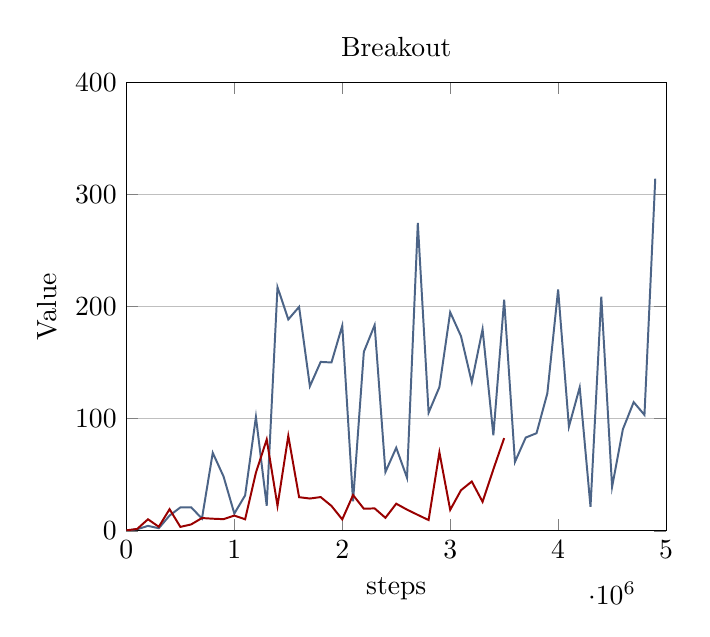
\begin{tikzpicture}

\begin{axis}[%
legend entries={rl-only-small-net,L2-reg,parallel-fs-50-no-aug}, 
legend columns=2,
title=Breakout,
legend to name=named,
legend style={legend cell align=left},
%%width=10in,
%%height=5in,
%%at={(2.596in,2.358in)},
% scale only axis,
xmin=0,
xmax=5000000,
xlabel style={font=\color{white!15!black}},
xlabel={steps},
xlabel near ticks,
ymin=0,
ymax=400,
ylabel style={font=\color{white!15!black}},
ylabel={Value},
ylabel near ticks,
ymajorgrids,
% %scale=0.5,
%%scale=0.4,
axis background/.style={fill=white},
%legend columns=2,
%legend=south outside
]
\addplot [color=blue, line width = 0.25mm]
                table[row sep=crcr]{
                  0 0.20000000298023224\\ 
100000 1.399999976158142\\ 
200000 4.400000095367432\\ 
300000 2.299999952316284\\ 
400000 13.600000381469727\\ 
500000 20.899999618530273\\ 
600000 21.0\\ 
700000 10.899999618530273\\ 
800000 69.5999984741211\\ 
900000 48.5\\ 
1000000 15.399999618530273\\ 
1100000 31.600000381469727\\ 
1200000 101.5999984741211\\ 
1300000 22.399999618530273\\ 
1400000 217.39999389648438\\ 
1500000 188.60000610351562\\ 
1600000 199.8000030517578\\ 
1700000 129.0\\ 
1800000 150.6999969482422\\ 
1900000 150.1999969482422\\ 
2000000 183.0\\ 
2100000 26.399999618530273\\ 
2200000 159.6999969482422\\ 
2300000 183.5\\ 
2400000 52.5\\ 
2500000 74.0999984741211\\ 
2600000 47.29999923706055\\ 
2700000 274.6000061035156\\ 
2800000 105.4000015258789\\ 
2900000 128.1999969482422\\ 
3000000 195.0\\ 
3100000 173.6999969482422\\ 
3200000 132.60000610351562\\ 
3300000 179.89999389648438\\ 
3400000 85.19999694824219\\ 
3500000 206.1999969482422\\ 
3600000 61.5\\ 
3700000 83.19999694824219\\ 
3800000 87.0999984741211\\ 
3900000 122.5999984741211\\ 
4000000 215.3000030517578\\ 
4100000 92.9000015258789\\ 
4200000 128.0\\ 
4300000 21.399999618530273\\ 
4400000 208.89999389648438\\ 
4500000 39.20000076293945\\ 
4600000 90.5999984741211\\ 
4700000 114.80000305175781\\ 
4800000 103.4000015258789\\ 
4900000 314.20001220703125\\ 
};
\addplot [color=red, line width = 0.25mm]
                table[row sep=crcr]{
                  0 0.4000000059604645\\ 
100000 1.7000000476837158\\ 
200000 10.300000190734863\\ 
300000 3.5999999046325684\\ 
400000 19.299999237060547\\ 
500000 3.5\\ 
600000 5.699999809265137\\ 
700000 11.399999618530273\\ 
800000 10.800000190734863\\ 
900000 10.399999618530273\\ 
1000000 13.600000381469727\\ 
1100000 10.300000190734863\\ 
1200000 51.900001525878906\\ 
1300000 81.5\\ 
1400000 22.299999237060547\\ 
1500000 84.69999694824219\\ 
1600000 30.0\\ 
1700000 28.799999237060547\\ 
1800000 30.100000381469727\\ 
1900000 22.200000762939453\\ 
2000000 10.199999809265137\\ 
2100000 31.899999618530273\\ 
2200000 19.700000762939453\\ 
2300000 20.0\\ 
2400000 11.600000381469727\\ 
2500000 24.200000762939453\\ 
2600000 18.899999618530273\\ 
2700000 14.199999809265137\\ 
2800000 9.600000381469727\\ 
2900000 70.0\\ 
3000000 18.700000762939453\\ 
3100000 36.20000076293945\\ 
3200000 44.0\\ 
3300000 25.899999618530273\\ 
3400000 54.900001525878906\\ 
3500000 82.69999694824219\\ 
};
\addplot [color=yellow, line width = 0.25mm]
                table[row sep=crcr]{
                  0 0.800000011920929\\ 
};
\end{axis}
\end{tikzpicture}}}
    \subfloat[]{  \resizebox{0.4\textwidth}{!}{
%\definecolor{blue}{RGB}{76,100,135}
%\definecolor{red}{RGB}{153,0,0}
%\definecolor{yellow}{RGB}{227,178,60}
%\definecolor{mycolor1}{rgb}{0.00000,0.44700,0.74100}%
%\definecolor{mycolor2}{rgb}{0.85000,0.32500,0.09800}%
%\definecolor{mycolor3}{rgb}{0.92900,0.69400,0.12500}%
%
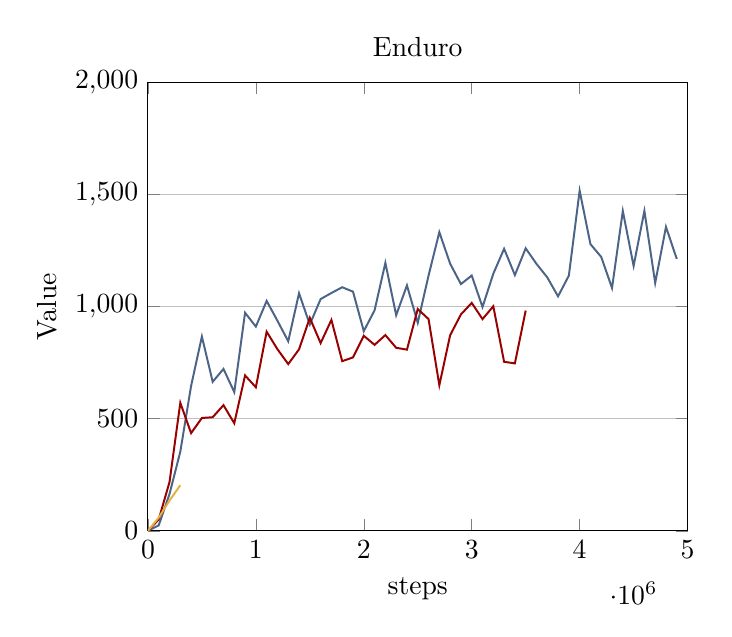
\begin{tikzpicture}

\begin{axis}[%
title=Enduro,
% %width=4.634in,
%%width=10in,
%%height=5in,
%at={(2.596in,2.358in)},
% scale only axis,
xmin=0,
xmax=5000000,
xlabel style={font=\color{white!15!black}},
xlabel={steps},
xlabel near ticks,
ymin=0,
ymax=2000,
ylabel style={font=\color{white!15!black}},
ylabel={Value},
ylabel near ticks,
ymajorgrids,
% %scale=0.5,
%scale=0.4,
axis background/.style={fill=white},
%legend style={legend cell align=left, align=left, draw=white!15!black}
]
\addplot [color=blue, line width = 0.25mm]
                table[row sep=crcr]{
                  0 0.0\\ 
100000 24.299999237060547\\ 
200000 164.3000030517578\\ 
300000 353.0\\ 
400000 646.4000244140625\\ 
500000 866.7000122070312\\ 
600000 664.7000122070312\\ 
700000 722.2000122070312\\ 
800000 618.9000244140625\\ 
900000 972.7999877929688\\ 
1000000 910.9000244140625\\ 
1100000 1025.699951171875\\ 
1200000 937.0\\ 
1300000 845.5999755859375\\ 
1400000 1059.9000244140625\\ 
1500000 920.2999877929688\\ 
1600000 1033.800048828125\\ 
1700000 1061.0\\ 
1800000 1086.5999755859375\\ 
1900000 1066.9000244140625\\ 
2000000 890.9000244140625\\ 
2100000 983.5\\ 
2200000 1195.300048828125\\ 
2300000 962.0\\ 
2400000 1094.800048828125\\ 
2500000 928.0\\ 
2600000 1138.5999755859375\\ 
2700000 1332.300048828125\\ 
2800000 1191.800048828125\\ 
2900000 1100.5999755859375\\ 
3000000 1138.800048828125\\ 
3100000 998.2999877929688\\ 
3200000 1146.800048828125\\ 
3300000 1258.0999755859375\\ 
3400000 1141.0\\ 
3500000 1260.300048828125\\ 
3600000 1190.800048828125\\ 
3700000 1130.5999755859375\\ 
3800000 1046.0999755859375\\ 
3900000 1138.4000244140625\\ 
4000000 1517.5\\ 
4100000 1278.9000244140625\\ 
4200000 1221.699951171875\\ 
4300000 1083.199951171875\\ 
4400000 1426.9000244140625\\ 
4500000 1181.5999755859375\\ 
4600000 1427.199951171875\\ 
4700000 1105.800048828125\\ 
4800000 1355.800048828125\\ 
4900000 1212.9000244140625\\ 
};
\addplot [color=red, line width = 0.25mm]
                table[row sep=crcr]{
                  0 0.0\\ 
100000 50.5\\ 
200000 217.60000610351562\\ 
300000 570.9000244140625\\ 
400000 435.6000061035156\\ 
500000 503.3999938964844\\ 
600000 506.79998779296875\\ 
700000 560.5\\ 
800000 479.79998779296875\\ 
900000 693.2000122070312\\ 
1000000 640.4000244140625\\ 
1100000 888.4000244140625\\ 
1200000 810.0999755859375\\ 
1300000 743.7999877929688\\ 
1400000 809.5\\ 
1500000 950.2000122070312\\ 
1600000 837.4000244140625\\ 
1700000 940.7999877929688\\ 
1800000 756.7999877929688\\ 
1900000 773.5\\ 
2000000 870.0999755859375\\ 
2100000 829.5999755859375\\ 
2200000 873.2000122070312\\ 
2300000 816.5\\ 
2400000 808.2000122070312\\ 
2500000 989.5999755859375\\ 
2600000 944.5\\ 
2700000 649.4000244140625\\ 
2800000 872.4000244140625\\ 
2900000 965.2000122070312\\ 
3000000 1016.7000122070312\\ 
3100000 944.4000244140625\\ 
3200000 1001.7000122070312\\ 
3300000 754.0\\ 
3400000 746.7999877929688\\ 
3500000 982.2999877929688\\ 
};
\addplot [color=yellow, line width = 0.25mm]
                table[row sep=crcr]{
                  0 0.0\\ 
100000 58.79999923706055\\ 
200000 135.10000610351562\\ 
300000 203.1999969482422\\ 
};
\end{axis}
\end{tikzpicture}}}\\
  \vspace{-1cm}
    \subfloat[]{  \resizebox{0.4\textwidth}{!}{
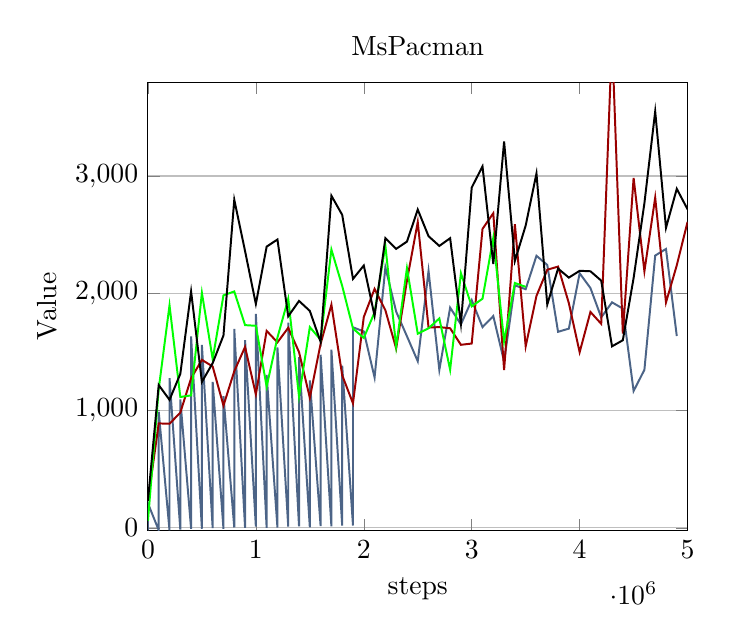
\begin{tikzpicture}

\begin{axis}[%
title=MsPacman,
% %width=4.634in,
%width=10in,
%height=5in,
%at={(2.596in,2.358in)},
% scale only axis,
xmin=0,
xmax=5000000,
xlabel style={font=\color{white!15!black}},
xlabel={steps},
xlabel near ticks,
ymin=-22,
ymax=3800,
ylabel style={font=\color{white!15!black}},
ylabel={Value},
ylabel near ticks,
ymajorgrids,
% %scale=0.5,
%scale=0.4,
axis background/.style={fill=white},
%legend style={legend cell align=left, align=left, draw=white!15!black}
]
\addplot [color=blue, line width = 0.25mm]
                table[row sep=crcr]{
                  0 -21.0\\ 
0 210.0\\ 
100000 -19.799999237060547\\ 
100000 990.0\\ 
200000 -20.700000762939453\\ 
200000 1277.0\\ 
300000 -15.0\\ 
300000 1096.0\\ 
400000 -7.0\\ 
400000 1632.0\\ 
500000 -6.900000095367432\\ 
500000 1561.0\\ 
600000 -1.899999976158142\\ 
600000 1245.0\\ 
700000 -7.599999904632568\\ 
700000 1123.0\\ 
800000 4.0\\ 
800000 1696.0\\ 
900000 1.5\\ 
900000 1600.0\\ 
1000000 11.300000190734863\\ 
1000000 1824.0\\ 
1100000 1.2000000476837158\\ 
1100000 1304.0\\ 
1200000 3.700000047683716\\ 
1200000 1538.0\\ 
1300000 11.5\\ 
1300000 1750.0\\ 
1400000 13.600000381469727\\ 
1400000 1456.0\\ 
1500000 5.699999809265137\\ 
1500000 1258.0\\ 
1600000 15.600000381469727\\ 
1600000 1476.0\\ 
1700000 13.5\\ 
1700000 1519.0\\ 
1800000 19.299999237060547\\ 
1800000 1383.0\\ 
1900000 20.799999237060547\\ 
1900000 1710.0\\ 
2000000 1675.0\\ 
2100000 1282.0\\ 
2200000 2222.0\\ 
2300000 1844.0\\ 
2400000 1634.0\\ 
2500000 1421.0\\ 
2600000 2191.0\\ 
2700000 1347.0\\ 
2800000 1878.0\\ 
2900000 1735.0\\ 
3000000 1942.0\\ 
3100000 1712.0\\ 
3200000 1806.0\\ 
3300000 1419.0\\ 
3400000 2068.0\\ 
3500000 2035.0\\ 
3600000 2320.0\\ 
3700000 2242.0\\ 
3800000 1672.0\\ 
3900000 1699.0\\ 
4000000 2171.0\\ 
4100000 2045.0\\ 
4200000 1795.0\\ 
4300000 1923.0\\ 
4400000 1870.0\\ 
4500000 1167.0\\ 
4600000 1348.0\\ 
4700000 2322.0\\ 
4800000 2378.0\\ 
4900000 1636.0\\ 
};
\addplot [color=red, line width = 0.25mm]
                table[row sep=crcr]{
                  0 230.0\\ 
100000 891.0\\ 
200000 888.0\\ 
300000 983.0\\ 
400000 1276.0\\ 
500000 1433.0\\ 
600000 1376.0\\ 
700000 1043.0\\ 
800000 1336.0\\ 
900000 1543.0\\ 
1000000 1139.0\\ 
1100000 1680.0\\ 
1200000 1582.0\\ 
1300000 1706.0\\ 
1400000 1499.0\\ 
1500000 1110.0\\ 
1600000 1569.0\\ 
1700000 1903.0\\ 
1800000 1301.0\\ 
1900000 1062.0\\ 
2000000 1798.0\\ 
2100000 2038.0\\ 
2200000 1856.0\\ 
2300000 1530.0\\ 
2400000 2109.0\\ 
2500000 2607.0\\ 
2600000 1708.0\\ 
2700000 1712.0\\ 
2800000 1702.0\\ 
2900000 1561.0\\ 
3000000 1572.0\\ 
3100000 2549.0\\ 
3200000 2683.0\\ 
3300000 1346.0\\ 
3400000 2590.0\\ 
3500000 1548.0\\ 
3600000 1978.0\\ 
3700000 2201.0\\ 
3800000 2228.0\\ 
3900000 1916.0\\ 
4000000 1498.0\\ 
4100000 1841.0\\ 
4200000 1740.0\\ 
4300000 4177.0\\ 
4400000 1656.0\\ 
4500000 2984.0\\ 
4600000 2188.0\\ 
4700000 2816.0\\ 
4800000 1922.0\\ 
4900000 2239.0\\ 
5000000 2609.0\\ 
};
\addplot [color=green, line width = 0.25mm]
                table[row sep=crcr]{
                  0 60.0\\ 
100000 1185.0\\ 
200000 1898.0\\ 
300000 1116.0\\ 
400000 1130.0\\ 
500000 2004.0\\ 
600000 1439.0\\ 
700000 1983.0\\ 
800000 2016.0\\ 
900000 1729.0\\ 
1000000 1723.0\\ 
1100000 1205.0\\ 
1200000 1623.0\\ 
1300000 1954.0\\ 
1400000 1121.0\\ 
1500000 1712.0\\ 
1600000 1604.0\\ 
1700000 2373.0\\ 
1800000 2063.0\\ 
1900000 1700.0\\ 
2000000 1620.0\\ 
2100000 1838.0\\ 
2200000 2406.0\\ 
2300000 1546.0\\ 
2400000 2215.0\\ 
2500000 1656.0\\ 
2600000 1702.0\\ 
2700000 1786.0\\ 
2800000 1348.0\\ 
2900000 2172.0\\ 
3000000 1889.0\\ 
3100000 1954.0\\ 
3200000 2473.0\\ 
3300000 1591.0\\ 
3400000 2088.0\\ 
3500000 2055.0\\ 
};
\addplot [color=black, line width = 0.25mm]
                table[row sep=crcr]{
                  0 230.0\\ 
100000 1218.0\\ 
200000 1092.0\\ 
300000 1313.0\\ 
400000 2016.0\\ 
500000 1245.0\\ 
600000 1405.0\\ 
700000 1641.0\\ 
800000 2798.0\\ 
900000 2360.0\\ 
1000000 1909.0\\ 
1100000 2398.0\\ 
1200000 2459.0\\ 
1300000 1804.0\\ 
1400000 1935.0\\ 
1500000 1850.0\\ 
1600000 1586.0\\ 
1700000 2832.0\\ 
1800000 2669.0\\ 
1900000 2123.0\\ 
2000000 2237.0\\ 
2100000 1808.0\\ 
2200000 2470.0\\ 
2300000 2379.0\\ 
2400000 2441.0\\ 
2500000 2714.0\\ 
2600000 2487.0\\ 
2700000 2404.0\\ 
2800000 2470.0\\ 
2900000 1739.0\\ 
3000000 2902.0\\ 
3100000 3082.0\\ 
3200000 2250.0\\ 
3300000 3294.0\\ 
3400000 2276.0\\ 
3500000 2578.0\\ 
3600000 3022.0\\ 
3700000 1904.0\\ 
3800000 2211.0\\ 
3900000 2134.0\\ 
4000000 2192.0\\ 
4100000 2188.0\\ 
4200000 2108.0\\ 
4300000 1548.0\\ 
4400000 1600.0\\ 
4500000 2130.0\\ 
4600000 2768.0\\ 
4700000 3551.0\\ 
4800000 2558.0\\ 
4900000 2891.0\\ 
5000000 2716.0\\ 
};
\end{axis}
\end{tikzpicture}}}
    \subfloat[]{  \resizebox{0.4\textwidth}{!}{
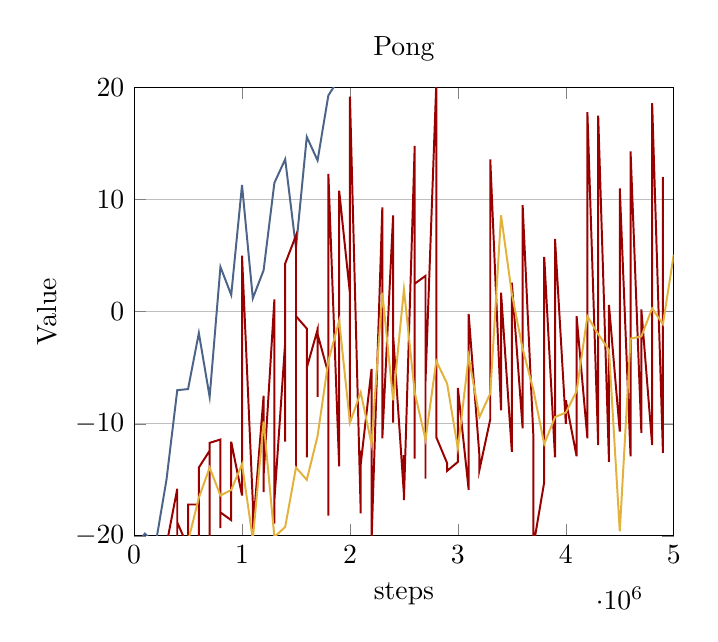
\begin{tikzpicture}

\begin{axis}[%
title=Pong,
% %width=4.634in,
%width=10in,
%height=5in,
%at={(2.596in,2.358in)},
% scale only axis,
xmin=0,
xmax=5000000,
xlabel style={font=\color{white!15!black}},
xlabel={steps},
xlabel near ticks,
ymin=-20,
ymax=20,
ylabel style={font=\color{white!15!black}},
ylabel={Value},
ylabel near ticks,
ymajorgrids,
% %scale=0.5,
%scale=0.4,
axis background/.style={fill=white},
%legend style={legend cell align=left, align=left, draw=white!15!black}
]
\addplot [color=blue, line width = 0.25mm]
                table[row sep=crcr]{
                  0 -21.0\\ 
100000 -19.799999237060547\\ 
200000 -20.700000762939453\\ 
300000 -15.0\\ 
400000 -7.0\\ 
500000 -6.900000095367432\\ 
600000 -1.899999976158142\\ 
700000 -7.599999904632568\\ 
800000 4.0\\ 
900000 1.5\\ 
1000000 11.300000190734863\\ 
1100000 1.2000000476837158\\ 
1200000 3.700000047683716\\ 
1300000 11.5\\ 
1400000 13.600000381469727\\ 
1500000 5.699999809265137\\ 
1600000 15.600000381469727\\ 
1700000 13.5\\ 
1800000 19.299999237060547\\ 
1900000 20.799999237060547\\ 
};
\addplot [color=red, line width = 0.25mm]
                table[row sep=crcr]{
                  0 -21.0\\ 
0 -21.0\\ 
0 -21.0\\ 
0 -21.0\\ 
100000 -21.0\\ 
100000 -20.600000381469727\\ 
100000 -21.0\\ 
200000 -20.399999618530273\\ 
200000 -21.0\\ 
200000 -20.799999237060547\\ 
300000 -20.600000381469727\\ 
300000 -20.799999237060547\\ 
300000 -20.799999237060547\\ 
400000 -15.800000190734863\\ 
400000 -20.399999618530273\\ 
400000 -18.799999237060547\\ 
500000 -21.0\\ 
500000 -21.0\\ 
500000 -17.200000762939453\\ 
600000 -17.200000762939453\\ 
600000 -20.600000381469727\\ 
600000 -13.899999618530273\\ 
700000 -12.399999618530273\\ 
700000 -20.100000381469727\\ 
700000 -11.699999809265137\\ 
800000 -11.399999618530273\\ 
800000 -19.299999237060547\\ 
800000 -17.899999618530273\\ 
900000 -18.600000381469727\\ 
900000 -15.699999809265137\\ 
900000 -11.600000381469727\\ 
1000000 -16.399999618530273\\ 
1000000 -16.0\\ 
1000000 5.0\\ 
1100000 -17.0\\ 
1100000 -17.5\\ 
1100000 -19.600000381469727\\ 
1200000 -7.5\\ 
1200000 -16.100000381469727\\ 
1200000 -14.600000381469727\\ 
1300000 1.100000023841858\\ 
1300000 -18.899999618530273\\ 
1300000 -16.799999237060547\\ 
1400000 -2.700000047683716\\ 
1400000 -11.600000381469727\\ 
1400000 4.300000190734863\\ 
1500000 6.800000190734863\\ 
1500000 -13.899999618530273\\ 
1500000 -0.4000000059604645\\ 
1600000 -1.5\\ 
1600000 -13.0\\ 
1600000 -5.0\\ 
1700000 -1.600000023841858\\ 
1700000 -7.599999904632568\\ 
1700000 -2.0\\ 
1800000 -5.5\\ 
1800000 -18.200000762939453\\ 
1800000 12.300000190734863\\ 
1900000 -13.800000190734863\\ 
1900000 -10.0\\ 
1900000 10.800000190734863\\ 
2000000 1.600000023841858\\ 
2000000 -9.899999618530273\\ 
2000000 19.200000762939453\\ 
2100000 -18.0\\ 
2100000 -12.399999618530273\\ 
2100000 -13.600000381469727\\ 
2200000 -5.099999904632568\\ 
2200000 -13.899999618530273\\ 
2200000 -20.5\\ 
2300000 9.300000190734863\\ 
2300000 -8.199999809265137\\ 
2300000 -11.300000190734863\\ 
2400000 8.600000381469727\\ 
2400000 -9.899999618530273\\ 
2400000 -2.0999999046325684\\ 
2500000 -16.299999237060547\\ 
2500000 -12.800000190734863\\ 
2500000 -16.799999237060547\\ 
2600000 14.800000190734863\\ 
2600000 -13.100000381469727\\ 
2600000 2.5\\ 
2700000 3.200000047683716\\ 
2700000 -14.899999618530273\\ 
2700000 -6.199999809265137\\ 
2800000 20.399999618530273\\ 
2800000 -9.800000190734863\\ 
2800000 -11.199999809265137\\ 
2900000 -13.5\\ 
2900000 -14.199999809265137\\ 
3000000 -13.399999618530273\\ 
3000000 -6.800000190734863\\ 
3100000 -15.899999618530273\\ 
3100000 -0.20000000298023224\\ 
3200000 -12.899999618530273\\ 
3200000 -14.100000381469727\\ 
3300000 -9.600000381469727\\ 
3300000 13.600000381469727\\ 
3400000 -8.800000190734863\\ 
3400000 1.7000000476837158\\ 
3500000 -12.5\\ 
3500000 2.5999999046325684\\ 
3600000 -10.399999618530273\\ 
3600000 9.5\\ 
3700000 -11.199999809265137\\ 
3700000 -20.899999618530273\\ 
3800000 -15.199999809265137\\ 
3800000 4.900000095367432\\ 
3900000 -13.0\\ 
3900000 6.5\\ 
4000000 -10.0\\ 
4000000 -7.900000095367432\\ 
4100000 -12.899999618530273\\ 
4100000 -0.4000000059604645\\ 
4200000 -11.300000190734863\\ 
4200000 17.799999237060547\\ 
4300000 -11.899999618530273\\ 
4300000 17.5\\ 
4400000 -13.399999618530273\\ 
4400000 0.6000000238418579\\ 
4500000 -10.699999809265137\\ 
4500000 11.0\\ 
4600000 -12.899999618530273\\ 
4600000 14.300000190734863\\ 
4700000 -10.800000190734863\\ 
4700000 0.20000000298023224\\ 
4800000 -11.899999618530273\\ 
4800000 18.600000381469727\\ 
4900000 -12.600000381469727\\ 
4900000 12.0\\ 
};
\addplot [color=yellow, line width = 0.25mm]
                table[row sep=crcr]{
                  0 -21.0\\ 
0 -21.0\\ 
100000 -21.0\\ 
200000 -21.0\\ 
300000 -20.399999618530273\\ 
400000 -21.0\\ 
500000 -20.5\\ 
600000 -16.600000381469727\\ 
700000 -13.899999618530273\\ 
800000 -16.399999618530273\\ 
900000 -15.899999618530273\\ 
1000000 -13.600000381469727\\ 
1100000 -20.299999237060547\\ 
1200000 -9.800000190734863\\ 
1300000 -20.100000381469727\\ 
1400000 -19.200000762939453\\ 
1500000 -13.899999618530273\\ 
1600000 -15.0\\ 
1700000 -11.100000381469727\\ 
1800000 -4.400000095367432\\ 
1900000 -0.800000011920929\\ 
2000000 -9.899999618530273\\ 
2100000 -7.199999809265137\\ 
2200000 -11.800000190734863\\ 
2300000 1.7000000476837158\\ 
2400000 -7.900000095367432\\ 
2500000 2.0\\ 
2600000 -7.199999809265137\\ 
2700000 -11.399999618530273\\ 
2800000 -4.400000095367432\\ 
2900000 -6.400000095367432\\ 
3000000 -12.199999809265137\\ 
3100000 -4.0\\ 
3200000 -9.399999618530273\\ 
3300000 -7.300000190734863\\ 
3400000 8.600000381469727\\ 
3500000 1.600000023841858\\ 
3600000 -3.299999952316284\\ 
3700000 -7.0\\ 
3800000 -11.800000190734863\\ 
3900000 -9.399999618530273\\ 
4000000 -9.0\\ 
4100000 -7.099999904632568\\ 
4200000 -0.4000000059604645\\ 
4300000 -2.0\\ 
4400000 -3.4000000953674316\\ 
4500000 -19.600000381469727\\ 
4600000 -2.4000000953674316\\ 
4700000 -2.200000047683716\\ 
4800000 0.30000001192092896\\ 
4900000 -1.100000023841858\\ 
5000000 5.099999904632568\\ 
};
\end{axis}
\end{tikzpicture}}}\\
  \vspace{-1cm}
    \subfloat[]{  \resizebox{0.4\textwidth}{!}{
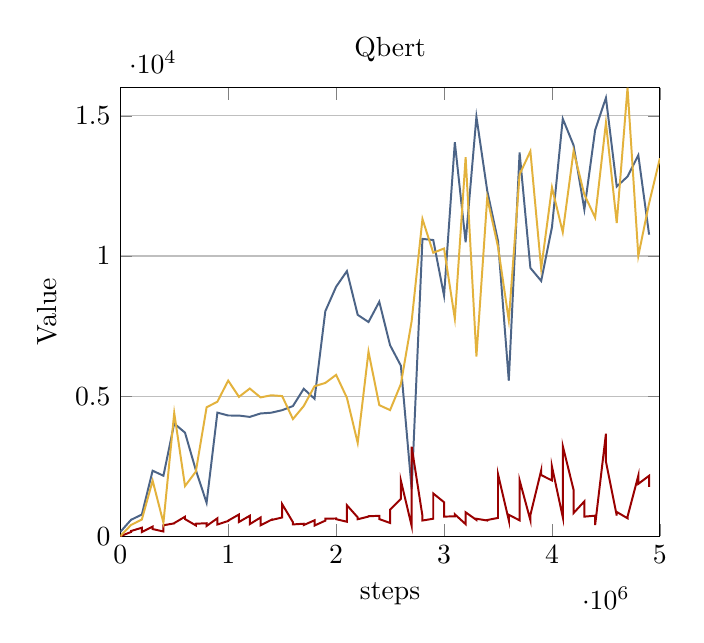
\begin{tikzpicture}

\begin{axis}[%
title=Qbert,
% %width=4.634in,
%width=10in,
%height=5in,
%at={(2.596in,2.358in)},
% scale only axis,
xmin=0,
xmax=5000000,
xlabel style={font=\color{white!15!black}},
xlabel={steps},
xlabel near ticks,
ymin=0,
ymax=16000,
ylabel style={font=\color{white!15!black}},
ylabel={Value},
ylabel near ticks,
ymajorgrids,
% %scale=0.5,
%scale=0.4,
axis background/.style={fill=white},
%legend style={legend cell align=left, align=left, draw=white!15!black}
]
\addplot [color=blue, line width = 0.25mm]
                table[row sep=crcr]{
                  0 150.0\\ 
100000 585.0\\ 
200000 772.5\\ 
300000 2337.5\\ 
400000 2157.5\\ 
500000 4022.5\\ 
600000 3695.0\\ 
700000 2362.5\\ 
800000 1192.5\\ 
900000 4410.0\\ 
1000000 4307.5\\ 
1100000 4305.0\\ 
1200000 4257.5\\ 
1300000 4380.0\\ 
1400000 4407.5\\ 
1500000 4497.5\\ 
1600000 4645.0\\ 
1700000 5260.0\\ 
1800000 4905.0\\ 
1900000 8030.0\\ 
2000000 8902.5\\ 
2100000 9460.0\\ 
2200000 7900.0\\ 
2300000 7642.5\\ 
2400000 8367.5\\ 
2500000 6815.0\\ 
2600000 6085.0\\ 
2700000 1677.5\\ 
2800000 10610.0\\ 
2900000 10570.0\\ 
3000000 8585.0\\ 
3100000 14057.5\\ 
3200000 10490.0\\ 
3300000 14970.0\\ 
3400000 12332.5\\ 
3500000 10537.5\\ 
3600000 5550.0\\ 
3700000 13692.5\\ 
3800000 9572.5\\ 
3900000 9110.0\\ 
4000000 11030.0\\ 
4100000 14897.5\\ 
4200000 13955.0\\ 
4300000 11660.0\\ 
4400000 14495.0\\ 
4500000 15645.0\\ 
4600000 12480.0\\ 
4700000 12835.0\\ 
4800000 13597.5\\ 
4900000 10762.5\\ 
};
\addplot [color=red, line width = 0.25mm]
                table[row sep=crcr]{
                  0 0.0\\ 
0 0.0\\ 
100000 150.0\\ 
100000 185.0\\ 
200000 302.5\\ 
200000 150.0\\ 
300000 342.5\\ 
300000 255.0\\ 
400000 167.5\\ 
400000 390.0\\ 
500000 457.5\\ 
500000 467.5\\ 
600000 695.0\\ 
600000 610.0\\ 
700000 385.0\\ 
700000 445.0\\ 
800000 462.5\\ 
800000 365.0\\ 
900000 640.0\\ 
900000 417.5\\ 
1000000 542.5\\ 
1000000 555.0\\ 
1100000 775.0\\ 
1100000 507.5\\ 
1200000 730.0\\ 
1200000 430.0\\ 
1300000 667.5\\ 
1300000 387.5\\ 
1400000 585.0\\ 
1400000 577.5\\ 
1500000 667.5\\ 
1500000 1145.0\\ 
1600000 500.0\\ 
1600000 420.0\\ 
1700000 445.0\\ 
1700000 397.5\\ 
1800000 567.5\\ 
1800000 380.0\\ 
1900000 555.0\\ 
1900000 625.0\\ 
2000000 632.5\\ 
2000000 607.5\\ 
2100000 515.0\\ 
2100000 1105.0\\ 
2200000 672.5\\ 
2200000 605.0\\ 
2300000 700.0\\ 
2300000 712.5\\ 
2400000 727.5\\ 
2400000 610.0\\ 
2500000 472.5\\ 
2500000 947.5\\ 
2600000 1330.0\\ 
2600000 1985.0\\ 
2700000 365.0\\ 
2700000 3195.0\\ 
2800000 720.0\\ 
2800000 560.0\\ 
2900000 622.5\\ 
2900000 1525.0\\ 
3000000 1212.5\\ 
3000000 700.0\\ 
3100000 707.5\\ 
3100000 780.0\\ 
3200000 430.0\\ 
3200000 852.5\\ 
3300000 580.0\\ 
3300000 622.5\\ 
3400000 560.0\\ 
3400000 577.5\\ 
3500000 652.5\\ 
3500000 2215.0\\ 
3600000 567.5\\ 
3600000 765.0\\ 
3700000 565.0\\ 
3700000 1995.0\\ 
3800000 570.0\\ 
3800000 757.5\\ 
3900000 2345.0\\ 
3900000 2182.5\\ 
4000000 1987.5\\ 
4000000 2482.5\\ 
4100000 682.5\\ 
4100000 3220.0\\ 
4200000 1657.5\\ 
4200000 825.0\\ 
4300000 1242.5\\ 
4300000 697.5\\ 
4400000 732.5\\ 
4400000 397.5\\ 
4500000 3660.0\\ 
4500000 2662.5\\ 
4600000 735.0\\ 
4600000 865.0\\ 
4700000 640.0\\ 
4700000 695.0\\ 
4800000 2160.0\\ 
4800000 1867.5\\ 
4900000 2157.5\\ 
4900000 1762.5\\ 
};
\addplot [color=yellow, line width = 0.25mm]
                table[row sep=crcr]{
                  0 0.0\\ 
0 0.0\\ 
0 0.0\\ 
0 0.0\\ 
100000 400.0\\ 
200000 595.0\\ 
300000 1982.5\\ 
400000 480.0\\ 
500000 4397.5\\ 
600000 1790.0\\ 
700000 2302.5\\ 
800000 4600.0\\ 
900000 4800.0\\ 
1000000 5552.5\\ 
1100000 4972.5\\ 
1200000 5270.0\\ 
1300000 4952.5\\ 
1400000 5030.0\\ 
1500000 5000.0\\ 
1600000 4180.0\\ 
1700000 4645.0\\ 
1800000 5352.5\\ 
1900000 5470.0\\ 
2000000 5757.5\\ 
2100000 4940.0\\ 
2200000 3327.5\\ 
2300000 6585.0\\ 
2400000 4677.5\\ 
2500000 4500.0\\ 
2600000 5430.0\\ 
2700000 7677.5\\ 
2800000 11320.0\\ 
2900000 10115.0\\ 
3000000 10267.5\\ 
3100000 7765.0\\ 
3200000 13525.0\\ 
3300000 6415.0\\ 
3400000 12077.5\\ 
3500000 10327.5\\ 
3600000 7700.0\\ 
3700000 12912.5\\ 
3800000 13737.5\\ 
3900000 9552.5\\ 
4000000 12445.0\\ 
4100000 10847.5\\ 
4200000 13737.5\\ 
4300000 12195.0\\ 
4400000 11370.0\\ 
4500000 14755.0\\ 
4600000 11175.0\\ 
4700000 16002.5\\ 
4800000 10005.0\\ 
4900000 11885.0\\ 
5000000 13490.0\\ 
};
\end{axis}
\end{tikzpicture}}}
    \subfloat[]{  \resizebox{0.4\textwidth}{!}{
\definecolor{blue}{RGB}{76,100,135}
\definecolor{red}{RGB}{153,0,0}
\definecolor{yellow}{RGB}{227,178,60}
\definecolor{mycolor1}{rgb}{0.00000,0.44700,0.74100}%
\definecolor{mycolor2}{rgb}{0.85000,0.32500,0.09800}%
\definecolor{mycolor3}{rgb}{0.92900,0.69400,0.12500}%
%
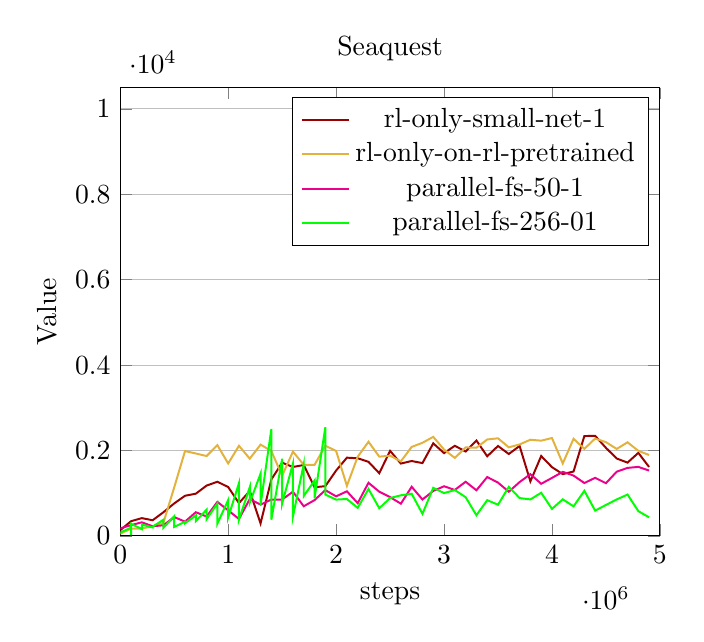
\begin{tikzpicture}

\begin{axis}[%
title=Seaquest,
% %width=4.634in,
%width=10in,
%height=5in,
%at={(2.596in,2.358in)},
% scale only axis,
xmin=0,
xmax=5000000,
xlabel style={font=\color{white!15!black}},
xlabel={steps},
xlabel near ticks,
ymin=0,
ymax=10500,
ylabel style={font=\color{white!15!black}},
ylabel={Value},
ylabel near ticks,
ymajorgrids,
% %scale=0.5,
%scale=0.4,
axis background/.style={fill=white},
%legend style={legend cell align=left, align=left, draw=white!15!black}
]
\addplot [color=red, line width = 0.25mm]
                table[row sep=crcr]{
                  0 134.0\\ 
100000 344.0\\ 
200000 416.0\\ 
300000 366.0\\ 
400000 554.0\\ 
500000 760.0\\ 
600000 940.0\\ 
700000 988.0\\ 
800000 1178.0\\ 
900000 1268.0\\ 
1000000 1144.0\\ 
1100000 768.0\\ 
1200000 1052.0\\ 
1300000 292.0\\ 
1400000 1322.0\\ 
1500000 1714.0\\ 
1600000 1614.0\\ 
1700000 1660.0\\ 
1800000 1140.0\\ 
1900000 1164.0\\ 
2000000 1530.0\\ 
2100000 1832.0\\ 
2200000 1818.0\\ 
2300000 1734.0\\ 
2400000 1468.0\\ 
2500000 1992.0\\ 
2600000 1694.0\\ 
2700000 1754.0\\ 
2800000 1704.0\\ 
2900000 2168.0\\ 
3000000 1938.0\\ 
3100000 2110.0\\ 
3200000 1976.0\\ 
3300000 2234.0\\ 
3400000 1864.0\\ 
3500000 2106.0\\ 
3600000 1918.0\\ 
3700000 2106.0\\ 
3800000 1276.0\\ 
3900000 1870.0\\ 
4000000 1610.0\\ 
4100000 1446.0\\ 
4200000 1508.0\\ 
4300000 2338.0\\ 
4400000 2344.0\\ 
4500000 2062.0\\ 
4600000 1812.0\\ 
4700000 1716.0\\ 
4800000 1944.0\\ 
4900000 1614.0\\ 
};
\addlegendentry{rl-only-small-net-1}
\addplot [color=yellow, line width = 0.25mm]
                table[row sep=crcr]{
                  0 48.0\\ 
100000 172.0\\ 
200000 172.0\\ 
300000 224.0\\ 
400000 308.0\\ 
500000 1136.0\\ 
600000 1986.0\\ 
700000 1930.0\\ 
800000 1870.0\\ 
900000 2124.0\\ 
1000000 1696.0\\ 
1100000 2110.0\\ 
1200000 1808.0\\ 
1300000 2138.0\\ 
1400000 1988.0\\ 
1500000 1408.0\\ 
1600000 1974.0\\ 
1700000 1664.0\\ 
1800000 1662.0\\ 
1900000 2112.0\\ 
2000000 1990.0\\ 
2100000 1172.0\\ 
2200000 1854.0\\ 
2300000 2204.0\\ 
2400000 1856.0\\ 
2500000 1878.0\\ 
2600000 1746.0\\ 
2700000 2084.0\\ 
2800000 2180.0\\ 
2900000 2320.0\\ 
3000000 2022.0\\ 
3100000 1826.0\\ 
3200000 2072.0\\ 
3300000 2064.0\\ 
3400000 2258.0\\ 
3500000 2286.0\\ 
3600000 2074.0\\ 
3700000 2142.0\\ 
3800000 2252.0\\ 
3900000 2230.0\\ 
4000000 2292.0\\ 
4100000 1696.0\\ 
4200000 2274.0\\ 
4300000 2038.0\\ 
4400000 2280.0\\ 
4500000 2196.0\\ 
4600000 2036.0\\ 
4700000 2192.0\\ 
4800000 1992.0\\ 
4900000 1894.0\\ 
};
\addlegendentry{rl-only-on-rl-pretrained}
\addplot [color=magenta, line width = 0.25mm]
                table[row sep=crcr]{
                  0 176.0\\ 
0 176.0\\ 
100000 252.0\\ 
200000 318.0\\ 
300000 226.0\\ 
400000 248.0\\ 
500000 440.0\\ 
600000 334.0\\ 
700000 554.0\\ 
800000 454.0\\ 
900000 796.0\\ 
1000000 598.0\\ 
1100000 396.0\\ 
1200000 862.0\\ 
1300000 732.0\\ 
1400000 850.0\\ 
1500000 852.0\\ 
1600000 1034.0\\ 
1700000 694.0\\ 
1800000 838.0\\ 
1900000 1072.0\\ 
2000000 926.0\\ 
2100000 1044.0\\ 
2200000 766.0\\ 
2300000 1244.0\\ 
2400000 1034.0\\ 
2500000 908.0\\ 
2600000 754.0\\ 
2700000 1150.0\\ 
2800000 852.0\\ 
2900000 1052.0\\ 
3000000 1162.0\\ 
3100000 1076.0\\ 
3200000 1268.0\\ 
3300000 1068.0\\ 
3400000 1378.0\\ 
3500000 1248.0\\ 
3600000 1034.0\\ 
3700000 1260.0\\ 
3800000 1446.0\\ 
3900000 1220.0\\ 
4000000 1358.0\\ 
4100000 1500.0\\ 
4200000 1412.0\\ 
4300000 1238.0\\ 
4400000 1360.0\\ 
4500000 1234.0\\ 
4600000 1504.0\\ 
4700000 1592.0\\ 
4800000 1616.0\\ 
4900000 1530.0\\ 
};
\addlegendentry{parallel-fs-50-1}
\addplot [color=green, line width = 0.25mm]
                table[row sep=crcr]{
                  0 80.0\\ 
0 80.0\\ 
0 80.0\\ 
100000 192.0\\ 
100000 20.0\\ 
100000 284.0\\ 
200000 158.0\\ 
200000 264.0\\ 
300000 198.0\\ 
300000 216.0\\ 
400000 378.0\\ 
400000 192.0\\ 
500000 460.0\\ 
500000 210.0\\ 
600000 330.0\\ 
600000 296.0\\ 
700000 478.0\\ 
700000 344.0\\ 
800000 614.0\\ 
800000 390.0\\ 
900000 758.0\\ 
900000 288.0\\ 
1000000 840.0\\ 
1000000 432.0\\ 
1100000 1236.0\\ 
1100000 384.0\\ 
1200000 1142.0\\ 
1200000 776.0\\ 
1300000 1458.0\\ 
1300000 730.0\\ 
1400000 2504.0\\ 
1400000 380.0\\ 
1500000 1806.0\\ 
1500000 756.0\\ 
1600000 1695.0\\ 
1600000 454.0\\ 
1700000 1678.0\\ 
1700000 932.0\\ 
1800000 1296.0\\ 
1800000 878.0\\ 
1900000 2544.0\\ 
1900000 968.0\\ 
2000000 850.0\\ 
2100000 864.0\\ 
2200000 656.0\\ 
2300000 1098.0\\ 
2400000 648.0\\ 
2500000 886.0\\ 
2600000 950.0\\ 
2700000 988.0\\ 
2800000 516.0\\ 
2900000 1126.0\\ 
3000000 1002.0\\ 
3100000 1074.0\\ 
3200000 906.0\\ 
3300000 484.0\\ 
3400000 836.0\\ 
3500000 730.0\\ 
3600000 1148.0\\ 
3700000 886.0\\ 
3800000 854.0\\ 
3900000 1010.0\\ 
4000000 632.0\\ 
4100000 856.0\\ 
4200000 692.0\\ 
4300000 1056.0\\ 
4400000 592.0\\ 
4500000 724.0\\ 
4600000 854.0\\ 
4700000 968.0\\ 
4800000 580.0\\ 
4900000 434.0\\ 
};
\addlegendentry{parallel-fs-256-01}
\end{axis}
\end{tikzpicture}}}\\
  \vspace{-1cm}
    \subfloat[]{  \resizebox{0.4\textwidth}{!}{
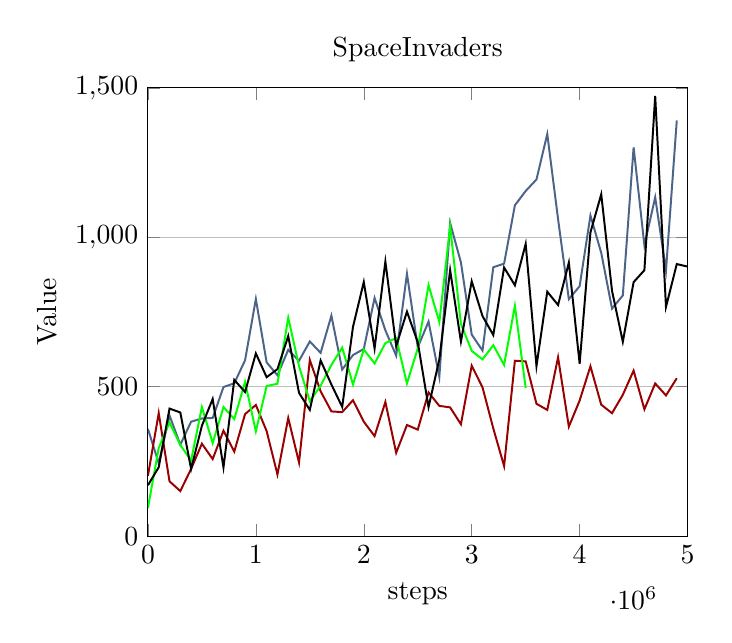
\begin{tikzpicture}

\begin{axis}[%
title=SpaceInvaders,
%width=10in,
%height=5in,
%at={(2.596in,2.358in)},
% scale only axis,
xmin=0,
xmax=5000000,
xlabel style={font=\color{white!15!black}},
xlabel={steps},
xlabel near ticks,
ymin=0,
ymax=1500,
ylabel style={font=\color{white!15!black}},
ylabel={Value},
ylabel near ticks,
ymajorgrids,
% %scale=0.5,
%scale=0.4,
axis background/.style={fill=white},
%legend style={legend cell align=left, align=left, draw=white!15!black}
]
\addplot [color=blue, line width = 0.25mm]
                table[row sep=crcr]{
                  0 359.0\\ 
100000 244.0\\ 
200000 404.0\\ 
300000 306.0\\ 
400000 383.0\\ 
500000 394.0\\ 
600000 395.5\\ 
700000 499.0\\ 
800000 511.5\\ 
900000 588.5\\ 
1000000 793.5\\ 
1100000 581.5\\ 
1200000 538.5\\ 
1300000 623.5\\ 
1400000 587.0\\ 
1500000 651.5\\ 
1600000 613.5\\ 
1700000 738.0\\ 
1800000 557.5\\ 
1900000 606.0\\ 
2000000 626.5\\ 
2100000 797.0\\ 
2200000 689.0\\ 
2300000 604.0\\ 
2400000 878.0\\ 
2500000 632.0\\ 
2600000 718.0\\ 
2700000 533.0\\ 
2800000 1048.0\\ 
2900000 916.0\\ 
3000000 674.5\\ 
3100000 621.0\\ 
3200000 900.0\\ 
3300000 912.0\\ 
3400000 1107.0\\ 
3500000 1155.0\\ 
3600000 1193.5\\ 
3700000 1345.5\\ 
3800000 1061.0\\ 
3900000 793.0\\ 
4000000 836.5\\ 
4100000 1073.0\\ 
4200000 948.0\\ 
4300000 761.5\\ 
4400000 805.5\\ 
4500000 1301.0\\ 
4600000 973.0\\ 
4700000 1134.0\\ 
4800000 889.5\\ 
4900000 1391.0\\ 
};
\addplot [color=red, line width = 0.25mm]
                table[row sep=crcr]{
                  0 202.0\\ 
100000 412.0\\ 
200000 183.5\\ 
300000 151.0\\ 
400000 225.0\\ 
500000 309.5\\ 
600000 258.0\\ 
700000 353.0\\ 
800000 283.0\\ 
900000 408.5\\ 
1000000 439.0\\ 
1100000 351.5\\ 
1200000 206.5\\ 
1300000 395.5\\ 
1400000 246.5\\ 
1500000 589.5\\ 
1600000 485.0\\ 
1700000 417.5\\ 
1800000 415.0\\ 
1900000 455.0\\ 
2000000 383.0\\ 
2100000 335.0\\ 
2200000 449.0\\ 
2300000 279.0\\ 
2400000 372.0\\ 
2500000 356.5\\ 
2600000 481.0\\ 
2700000 436.0\\ 
2800000 431.0\\ 
2900000 374.5\\ 
3000000 570.5\\ 
3100000 498.0\\ 
3200000 360.5\\ 
3300000 234.5\\ 
3400000 587.0\\ 
3500000 585.0\\ 
3600000 443.0\\ 
3700000 422.5\\ 
3800000 598.5\\ 
3900000 366.5\\ 
4000000 454.0\\ 
4100000 568.5\\ 
4200000 440.0\\ 
4300000 411.5\\ 
4400000 473.0\\ 
4500000 554.0\\ 
4600000 424.5\\ 
4700000 511.0\\ 
4800000 471.0\\ 
4900000 528.5\\ 
};
\addplot [color=green, line width = 0.25mm]
                table[row sep=crcr]{
                  0 94.5\\ 
100000 295.0\\ 
200000 380.5\\ 
300000 305.0\\ 
400000 253.0\\ 
500000 432.0\\ 
600000 311.5\\ 
700000 432.0\\ 
800000 392.0\\ 
900000 516.0\\ 
1000000 351.0\\ 
1100000 502.5\\ 
1200000 510.0\\ 
1300000 731.0\\ 
1400000 569.0\\ 
1500000 451.5\\ 
1600000 503.5\\ 
1700000 573.0\\ 
1800000 631.0\\ 
1900000 507.5\\ 
2000000 624.5\\ 
2100000 578.0\\ 
2200000 646.0\\ 
2300000 663.0\\ 
2400000 511.0\\ 
2500000 628.0\\ 
2600000 840.0\\ 
2700000 716.5\\ 
2800000 1037.0\\ 
2900000 710.5\\ 
3000000 620.0\\ 
3100000 591.5\\ 
3200000 639.0\\ 
3300000 573.0\\ 
3400000 771.0\\ 
3500000 496.0\\ 
};
\addplot [color=black, line width = 0.25mm]
                table[row sep=crcr]{
                  0 170.5\\ 
100000 230.5\\ 
200000 427.0\\ 
300000 414.0\\ 
400000 225.0\\ 
500000 369.5\\ 
600000 459.0\\ 
700000 230.0\\ 
800000 523.0\\ 
900000 482.5\\ 
1000000 611.5\\ 
1100000 532.0\\ 
1200000 559.0\\ 
1300000 669.5\\ 
1400000 479.5\\ 
1500000 422.5\\ 
1600000 588.0\\ 
1700000 507.5\\ 
1800000 432.5\\ 
1900000 700.5\\ 
2000000 850.5\\ 
2100000 628.0\\ 
2200000 919.0\\ 
2300000 636.0\\ 
2400000 751.5\\ 
2500000 649.0\\ 
2600000 432.0\\ 
2700000 591.5\\ 
2800000 890.0\\ 
2900000 651.0\\ 
3000000 853.0\\ 
3100000 736.5\\ 
3200000 673.0\\ 
3300000 899.0\\ 
3400000 839.5\\ 
3500000 978.0\\ 
3600000 569.0\\ 
3700000 818.0\\ 
3800000 773.5\\ 
3900000 915.5\\ 
4000000 577.0\\ 
4100000 1016.5\\ 
4200000 1144.0\\ 
4300000 821.0\\ 
4400000 650.5\\ 
4500000 850.0\\ 
4600000 890.0\\ 
4700000 1473.0\\ 
4800000 767.0\\ 
4900000 910.5\\ 
5000000 902.0\\ 
};
\end{axis}
\end{tikzpicture}}}
    \\

    \ref{named}
  \caption{Runs with Rainbow only, but with different encoder sizes. As can be seen,
  some games strongly benefit from having a larger encoder, while learning
fails on others.}
  \label{fig:big-vs-small-enc-rl-only}
\end{figure}

As can be seen in \ref{fig:big-vs-small-enc-rl-only}, some games benefit greatly from
having a large encoder (ex. Seaquest), while learning completely fails on others 
(ex. Breakout).
Despite rising the variance of the final result, the effect seems to be neutral
overall.



\section{Effectiveness of continuous updates}
\label{sec-effectiveness-of-parallel}
Having seen the effect of having pretrained encoders, we turn the attention
to the effect of continuous updating of the encoder with reconstruction loss.
The results are shown in \ref{fig-parallel}.

\begin{figure}[!t]
  \captionsetup[subfloat]{position=top,labelformat=empty}
  \vspace{-1.5cm}
  \centering

    \subfloat[]{  \resizebox{0.4\textwidth}{!}{
%\definecolor{blue}{RGB}{76,100,135}
%\definecolor{red}{RGB}{153,0,0}
%\definecolor{yellow}{RGB}{227,178,60}
%\definecolor{mycolor1}{rgb}{0.00000,0.44700,0.74100}%
%\definecolor{mycolor2}{rgb}{0.85000,0.32500,0.09800}%
%\definecolor{mycolor3}{rgb}{0.92900,0.69400,0.12500}%
%
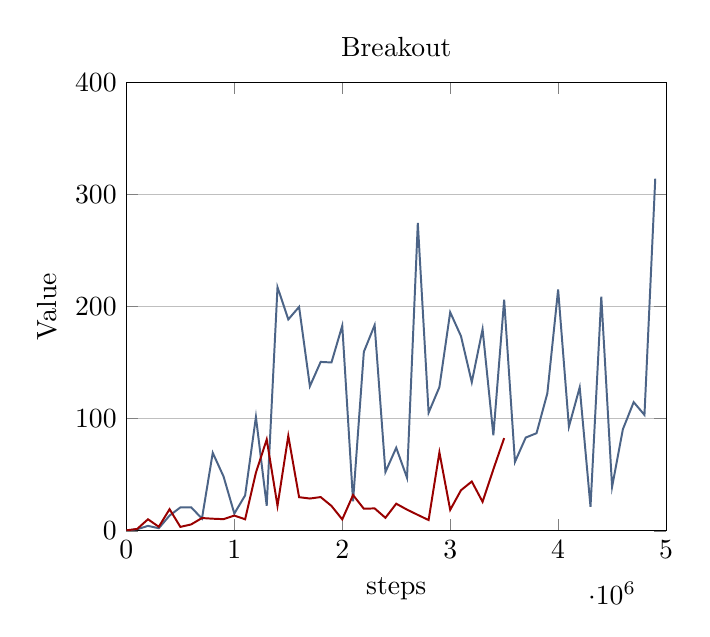
\begin{tikzpicture}

\begin{axis}[%
legend entries={rl-only-small-net,L2-reg,parallel-fs-50-no-aug}, 
legend columns=2,
title=Breakout,
legend to name=named,
legend style={legend cell align=left},
%%width=10in,
%%height=5in,
%%at={(2.596in,2.358in)},
% scale only axis,
xmin=0,
xmax=5000000,
xlabel style={font=\color{white!15!black}},
xlabel={steps},
xlabel near ticks,
ymin=0,
ymax=400,
ylabel style={font=\color{white!15!black}},
ylabel={Value},
ylabel near ticks,
ymajorgrids,
% %scale=0.5,
%%scale=0.4,
axis background/.style={fill=white},
%legend columns=2,
%legend=south outside
]
\addplot [color=blue, line width = 0.25mm]
                table[row sep=crcr]{
                  0 0.20000000298023224\\ 
100000 1.399999976158142\\ 
200000 4.400000095367432\\ 
300000 2.299999952316284\\ 
400000 13.600000381469727\\ 
500000 20.899999618530273\\ 
600000 21.0\\ 
700000 10.899999618530273\\ 
800000 69.5999984741211\\ 
900000 48.5\\ 
1000000 15.399999618530273\\ 
1100000 31.600000381469727\\ 
1200000 101.5999984741211\\ 
1300000 22.399999618530273\\ 
1400000 217.39999389648438\\ 
1500000 188.60000610351562\\ 
1600000 199.8000030517578\\ 
1700000 129.0\\ 
1800000 150.6999969482422\\ 
1900000 150.1999969482422\\ 
2000000 183.0\\ 
2100000 26.399999618530273\\ 
2200000 159.6999969482422\\ 
2300000 183.5\\ 
2400000 52.5\\ 
2500000 74.0999984741211\\ 
2600000 47.29999923706055\\ 
2700000 274.6000061035156\\ 
2800000 105.4000015258789\\ 
2900000 128.1999969482422\\ 
3000000 195.0\\ 
3100000 173.6999969482422\\ 
3200000 132.60000610351562\\ 
3300000 179.89999389648438\\ 
3400000 85.19999694824219\\ 
3500000 206.1999969482422\\ 
3600000 61.5\\ 
3700000 83.19999694824219\\ 
3800000 87.0999984741211\\ 
3900000 122.5999984741211\\ 
4000000 215.3000030517578\\ 
4100000 92.9000015258789\\ 
4200000 128.0\\ 
4300000 21.399999618530273\\ 
4400000 208.89999389648438\\ 
4500000 39.20000076293945\\ 
4600000 90.5999984741211\\ 
4700000 114.80000305175781\\ 
4800000 103.4000015258789\\ 
4900000 314.20001220703125\\ 
};
\addplot [color=red, line width = 0.25mm]
                table[row sep=crcr]{
                  0 0.4000000059604645\\ 
100000 1.7000000476837158\\ 
200000 10.300000190734863\\ 
300000 3.5999999046325684\\ 
400000 19.299999237060547\\ 
500000 3.5\\ 
600000 5.699999809265137\\ 
700000 11.399999618530273\\ 
800000 10.800000190734863\\ 
900000 10.399999618530273\\ 
1000000 13.600000381469727\\ 
1100000 10.300000190734863\\ 
1200000 51.900001525878906\\ 
1300000 81.5\\ 
1400000 22.299999237060547\\ 
1500000 84.69999694824219\\ 
1600000 30.0\\ 
1700000 28.799999237060547\\ 
1800000 30.100000381469727\\ 
1900000 22.200000762939453\\ 
2000000 10.199999809265137\\ 
2100000 31.899999618530273\\ 
2200000 19.700000762939453\\ 
2300000 20.0\\ 
2400000 11.600000381469727\\ 
2500000 24.200000762939453\\ 
2600000 18.899999618530273\\ 
2700000 14.199999809265137\\ 
2800000 9.600000381469727\\ 
2900000 70.0\\ 
3000000 18.700000762939453\\ 
3100000 36.20000076293945\\ 
3200000 44.0\\ 
3300000 25.899999618530273\\ 
3400000 54.900001525878906\\ 
3500000 82.69999694824219\\ 
};
\addplot [color=yellow, line width = 0.25mm]
                table[row sep=crcr]{
                  0 0.800000011920929\\ 
};
\end{axis}
\end{tikzpicture}}}
    \subfloat[]{  \resizebox{0.4\textwidth}{!}{
%\definecolor{blue}{RGB}{76,100,135}
%\definecolor{red}{RGB}{153,0,0}
%\definecolor{yellow}{RGB}{227,178,60}
%\definecolor{mycolor1}{rgb}{0.00000,0.44700,0.74100}%
%\definecolor{mycolor2}{rgb}{0.85000,0.32500,0.09800}%
%\definecolor{mycolor3}{rgb}{0.92900,0.69400,0.12500}%
%
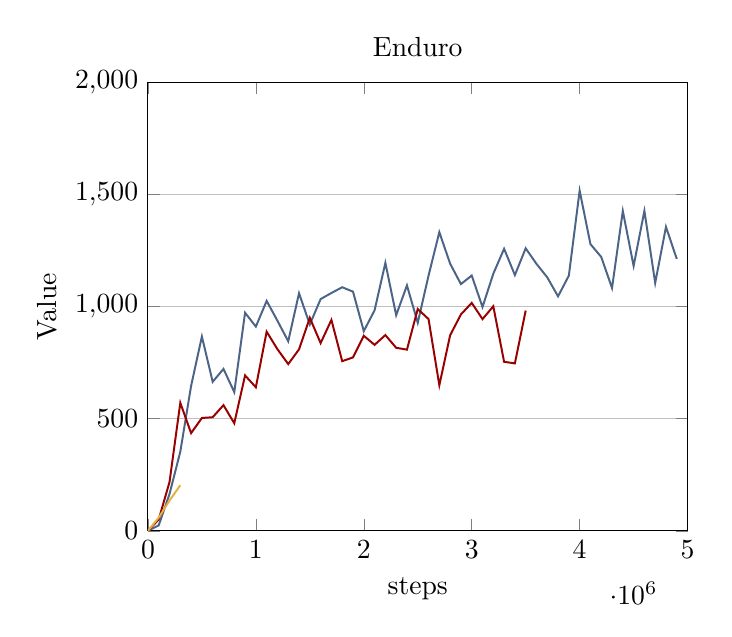
\begin{tikzpicture}

\begin{axis}[%
title=Enduro,
% %width=4.634in,
%%width=10in,
%%height=5in,
%at={(2.596in,2.358in)},
% scale only axis,
xmin=0,
xmax=5000000,
xlabel style={font=\color{white!15!black}},
xlabel={steps},
xlabel near ticks,
ymin=0,
ymax=2000,
ylabel style={font=\color{white!15!black}},
ylabel={Value},
ylabel near ticks,
ymajorgrids,
% %scale=0.5,
%scale=0.4,
axis background/.style={fill=white},
%legend style={legend cell align=left, align=left, draw=white!15!black}
]
\addplot [color=blue, line width = 0.25mm]
                table[row sep=crcr]{
                  0 0.0\\ 
100000 24.299999237060547\\ 
200000 164.3000030517578\\ 
300000 353.0\\ 
400000 646.4000244140625\\ 
500000 866.7000122070312\\ 
600000 664.7000122070312\\ 
700000 722.2000122070312\\ 
800000 618.9000244140625\\ 
900000 972.7999877929688\\ 
1000000 910.9000244140625\\ 
1100000 1025.699951171875\\ 
1200000 937.0\\ 
1300000 845.5999755859375\\ 
1400000 1059.9000244140625\\ 
1500000 920.2999877929688\\ 
1600000 1033.800048828125\\ 
1700000 1061.0\\ 
1800000 1086.5999755859375\\ 
1900000 1066.9000244140625\\ 
2000000 890.9000244140625\\ 
2100000 983.5\\ 
2200000 1195.300048828125\\ 
2300000 962.0\\ 
2400000 1094.800048828125\\ 
2500000 928.0\\ 
2600000 1138.5999755859375\\ 
2700000 1332.300048828125\\ 
2800000 1191.800048828125\\ 
2900000 1100.5999755859375\\ 
3000000 1138.800048828125\\ 
3100000 998.2999877929688\\ 
3200000 1146.800048828125\\ 
3300000 1258.0999755859375\\ 
3400000 1141.0\\ 
3500000 1260.300048828125\\ 
3600000 1190.800048828125\\ 
3700000 1130.5999755859375\\ 
3800000 1046.0999755859375\\ 
3900000 1138.4000244140625\\ 
4000000 1517.5\\ 
4100000 1278.9000244140625\\ 
4200000 1221.699951171875\\ 
4300000 1083.199951171875\\ 
4400000 1426.9000244140625\\ 
4500000 1181.5999755859375\\ 
4600000 1427.199951171875\\ 
4700000 1105.800048828125\\ 
4800000 1355.800048828125\\ 
4900000 1212.9000244140625\\ 
};
\addplot [color=red, line width = 0.25mm]
                table[row sep=crcr]{
                  0 0.0\\ 
100000 50.5\\ 
200000 217.60000610351562\\ 
300000 570.9000244140625\\ 
400000 435.6000061035156\\ 
500000 503.3999938964844\\ 
600000 506.79998779296875\\ 
700000 560.5\\ 
800000 479.79998779296875\\ 
900000 693.2000122070312\\ 
1000000 640.4000244140625\\ 
1100000 888.4000244140625\\ 
1200000 810.0999755859375\\ 
1300000 743.7999877929688\\ 
1400000 809.5\\ 
1500000 950.2000122070312\\ 
1600000 837.4000244140625\\ 
1700000 940.7999877929688\\ 
1800000 756.7999877929688\\ 
1900000 773.5\\ 
2000000 870.0999755859375\\ 
2100000 829.5999755859375\\ 
2200000 873.2000122070312\\ 
2300000 816.5\\ 
2400000 808.2000122070312\\ 
2500000 989.5999755859375\\ 
2600000 944.5\\ 
2700000 649.4000244140625\\ 
2800000 872.4000244140625\\ 
2900000 965.2000122070312\\ 
3000000 1016.7000122070312\\ 
3100000 944.4000244140625\\ 
3200000 1001.7000122070312\\ 
3300000 754.0\\ 
3400000 746.7999877929688\\ 
3500000 982.2999877929688\\ 
};
\addplot [color=yellow, line width = 0.25mm]
                table[row sep=crcr]{
                  0 0.0\\ 
100000 58.79999923706055\\ 
200000 135.10000610351562\\ 
300000 203.1999969482422\\ 
};
\end{axis}
\end{tikzpicture}}}\\
  \vspace{-1cm}
    \subfloat[]{  \resizebox{0.4\textwidth}{!}{
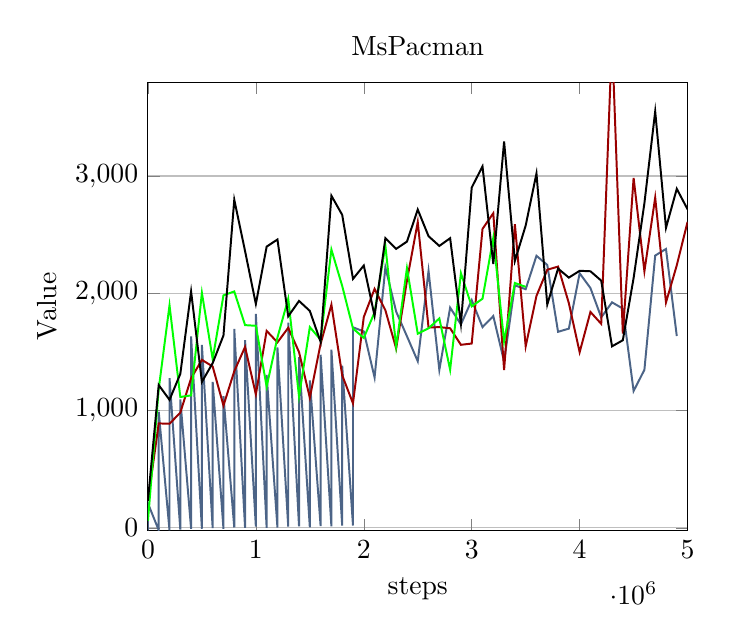
\begin{tikzpicture}

\begin{axis}[%
title=MsPacman,
% %width=4.634in,
%width=10in,
%height=5in,
%at={(2.596in,2.358in)},
% scale only axis,
xmin=0,
xmax=5000000,
xlabel style={font=\color{white!15!black}},
xlabel={steps},
xlabel near ticks,
ymin=-22,
ymax=3800,
ylabel style={font=\color{white!15!black}},
ylabel={Value},
ylabel near ticks,
ymajorgrids,
% %scale=0.5,
%scale=0.4,
axis background/.style={fill=white},
%legend style={legend cell align=left, align=left, draw=white!15!black}
]
\addplot [color=blue, line width = 0.25mm]
                table[row sep=crcr]{
                  0 -21.0\\ 
0 210.0\\ 
100000 -19.799999237060547\\ 
100000 990.0\\ 
200000 -20.700000762939453\\ 
200000 1277.0\\ 
300000 -15.0\\ 
300000 1096.0\\ 
400000 -7.0\\ 
400000 1632.0\\ 
500000 -6.900000095367432\\ 
500000 1561.0\\ 
600000 -1.899999976158142\\ 
600000 1245.0\\ 
700000 -7.599999904632568\\ 
700000 1123.0\\ 
800000 4.0\\ 
800000 1696.0\\ 
900000 1.5\\ 
900000 1600.0\\ 
1000000 11.300000190734863\\ 
1000000 1824.0\\ 
1100000 1.2000000476837158\\ 
1100000 1304.0\\ 
1200000 3.700000047683716\\ 
1200000 1538.0\\ 
1300000 11.5\\ 
1300000 1750.0\\ 
1400000 13.600000381469727\\ 
1400000 1456.0\\ 
1500000 5.699999809265137\\ 
1500000 1258.0\\ 
1600000 15.600000381469727\\ 
1600000 1476.0\\ 
1700000 13.5\\ 
1700000 1519.0\\ 
1800000 19.299999237060547\\ 
1800000 1383.0\\ 
1900000 20.799999237060547\\ 
1900000 1710.0\\ 
2000000 1675.0\\ 
2100000 1282.0\\ 
2200000 2222.0\\ 
2300000 1844.0\\ 
2400000 1634.0\\ 
2500000 1421.0\\ 
2600000 2191.0\\ 
2700000 1347.0\\ 
2800000 1878.0\\ 
2900000 1735.0\\ 
3000000 1942.0\\ 
3100000 1712.0\\ 
3200000 1806.0\\ 
3300000 1419.0\\ 
3400000 2068.0\\ 
3500000 2035.0\\ 
3600000 2320.0\\ 
3700000 2242.0\\ 
3800000 1672.0\\ 
3900000 1699.0\\ 
4000000 2171.0\\ 
4100000 2045.0\\ 
4200000 1795.0\\ 
4300000 1923.0\\ 
4400000 1870.0\\ 
4500000 1167.0\\ 
4600000 1348.0\\ 
4700000 2322.0\\ 
4800000 2378.0\\ 
4900000 1636.0\\ 
};
\addplot [color=red, line width = 0.25mm]
                table[row sep=crcr]{
                  0 230.0\\ 
100000 891.0\\ 
200000 888.0\\ 
300000 983.0\\ 
400000 1276.0\\ 
500000 1433.0\\ 
600000 1376.0\\ 
700000 1043.0\\ 
800000 1336.0\\ 
900000 1543.0\\ 
1000000 1139.0\\ 
1100000 1680.0\\ 
1200000 1582.0\\ 
1300000 1706.0\\ 
1400000 1499.0\\ 
1500000 1110.0\\ 
1600000 1569.0\\ 
1700000 1903.0\\ 
1800000 1301.0\\ 
1900000 1062.0\\ 
2000000 1798.0\\ 
2100000 2038.0\\ 
2200000 1856.0\\ 
2300000 1530.0\\ 
2400000 2109.0\\ 
2500000 2607.0\\ 
2600000 1708.0\\ 
2700000 1712.0\\ 
2800000 1702.0\\ 
2900000 1561.0\\ 
3000000 1572.0\\ 
3100000 2549.0\\ 
3200000 2683.0\\ 
3300000 1346.0\\ 
3400000 2590.0\\ 
3500000 1548.0\\ 
3600000 1978.0\\ 
3700000 2201.0\\ 
3800000 2228.0\\ 
3900000 1916.0\\ 
4000000 1498.0\\ 
4100000 1841.0\\ 
4200000 1740.0\\ 
4300000 4177.0\\ 
4400000 1656.0\\ 
4500000 2984.0\\ 
4600000 2188.0\\ 
4700000 2816.0\\ 
4800000 1922.0\\ 
4900000 2239.0\\ 
5000000 2609.0\\ 
};
\addplot [color=green, line width = 0.25mm]
                table[row sep=crcr]{
                  0 60.0\\ 
100000 1185.0\\ 
200000 1898.0\\ 
300000 1116.0\\ 
400000 1130.0\\ 
500000 2004.0\\ 
600000 1439.0\\ 
700000 1983.0\\ 
800000 2016.0\\ 
900000 1729.0\\ 
1000000 1723.0\\ 
1100000 1205.0\\ 
1200000 1623.0\\ 
1300000 1954.0\\ 
1400000 1121.0\\ 
1500000 1712.0\\ 
1600000 1604.0\\ 
1700000 2373.0\\ 
1800000 2063.0\\ 
1900000 1700.0\\ 
2000000 1620.0\\ 
2100000 1838.0\\ 
2200000 2406.0\\ 
2300000 1546.0\\ 
2400000 2215.0\\ 
2500000 1656.0\\ 
2600000 1702.0\\ 
2700000 1786.0\\ 
2800000 1348.0\\ 
2900000 2172.0\\ 
3000000 1889.0\\ 
3100000 1954.0\\ 
3200000 2473.0\\ 
3300000 1591.0\\ 
3400000 2088.0\\ 
3500000 2055.0\\ 
};
\addplot [color=black, line width = 0.25mm]
                table[row sep=crcr]{
                  0 230.0\\ 
100000 1218.0\\ 
200000 1092.0\\ 
300000 1313.0\\ 
400000 2016.0\\ 
500000 1245.0\\ 
600000 1405.0\\ 
700000 1641.0\\ 
800000 2798.0\\ 
900000 2360.0\\ 
1000000 1909.0\\ 
1100000 2398.0\\ 
1200000 2459.0\\ 
1300000 1804.0\\ 
1400000 1935.0\\ 
1500000 1850.0\\ 
1600000 1586.0\\ 
1700000 2832.0\\ 
1800000 2669.0\\ 
1900000 2123.0\\ 
2000000 2237.0\\ 
2100000 1808.0\\ 
2200000 2470.0\\ 
2300000 2379.0\\ 
2400000 2441.0\\ 
2500000 2714.0\\ 
2600000 2487.0\\ 
2700000 2404.0\\ 
2800000 2470.0\\ 
2900000 1739.0\\ 
3000000 2902.0\\ 
3100000 3082.0\\ 
3200000 2250.0\\ 
3300000 3294.0\\ 
3400000 2276.0\\ 
3500000 2578.0\\ 
3600000 3022.0\\ 
3700000 1904.0\\ 
3800000 2211.0\\ 
3900000 2134.0\\ 
4000000 2192.0\\ 
4100000 2188.0\\ 
4200000 2108.0\\ 
4300000 1548.0\\ 
4400000 1600.0\\ 
4500000 2130.0\\ 
4600000 2768.0\\ 
4700000 3551.0\\ 
4800000 2558.0\\ 
4900000 2891.0\\ 
5000000 2716.0\\ 
};
\end{axis}
\end{tikzpicture}}}
    \subfloat[]{  \resizebox{0.4\textwidth}{!}{
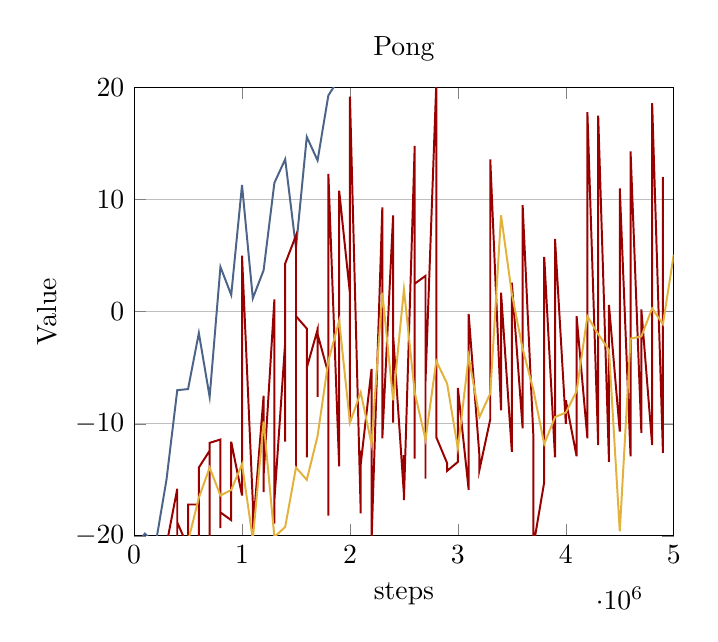
\begin{tikzpicture}

\begin{axis}[%
title=Pong,
% %width=4.634in,
%width=10in,
%height=5in,
%at={(2.596in,2.358in)},
% scale only axis,
xmin=0,
xmax=5000000,
xlabel style={font=\color{white!15!black}},
xlabel={steps},
xlabel near ticks,
ymin=-20,
ymax=20,
ylabel style={font=\color{white!15!black}},
ylabel={Value},
ylabel near ticks,
ymajorgrids,
% %scale=0.5,
%scale=0.4,
axis background/.style={fill=white},
%legend style={legend cell align=left, align=left, draw=white!15!black}
]
\addplot [color=blue, line width = 0.25mm]
                table[row sep=crcr]{
                  0 -21.0\\ 
100000 -19.799999237060547\\ 
200000 -20.700000762939453\\ 
300000 -15.0\\ 
400000 -7.0\\ 
500000 -6.900000095367432\\ 
600000 -1.899999976158142\\ 
700000 -7.599999904632568\\ 
800000 4.0\\ 
900000 1.5\\ 
1000000 11.300000190734863\\ 
1100000 1.2000000476837158\\ 
1200000 3.700000047683716\\ 
1300000 11.5\\ 
1400000 13.600000381469727\\ 
1500000 5.699999809265137\\ 
1600000 15.600000381469727\\ 
1700000 13.5\\ 
1800000 19.299999237060547\\ 
1900000 20.799999237060547\\ 
};
\addplot [color=red, line width = 0.25mm]
                table[row sep=crcr]{
                  0 -21.0\\ 
0 -21.0\\ 
0 -21.0\\ 
0 -21.0\\ 
100000 -21.0\\ 
100000 -20.600000381469727\\ 
100000 -21.0\\ 
200000 -20.399999618530273\\ 
200000 -21.0\\ 
200000 -20.799999237060547\\ 
300000 -20.600000381469727\\ 
300000 -20.799999237060547\\ 
300000 -20.799999237060547\\ 
400000 -15.800000190734863\\ 
400000 -20.399999618530273\\ 
400000 -18.799999237060547\\ 
500000 -21.0\\ 
500000 -21.0\\ 
500000 -17.200000762939453\\ 
600000 -17.200000762939453\\ 
600000 -20.600000381469727\\ 
600000 -13.899999618530273\\ 
700000 -12.399999618530273\\ 
700000 -20.100000381469727\\ 
700000 -11.699999809265137\\ 
800000 -11.399999618530273\\ 
800000 -19.299999237060547\\ 
800000 -17.899999618530273\\ 
900000 -18.600000381469727\\ 
900000 -15.699999809265137\\ 
900000 -11.600000381469727\\ 
1000000 -16.399999618530273\\ 
1000000 -16.0\\ 
1000000 5.0\\ 
1100000 -17.0\\ 
1100000 -17.5\\ 
1100000 -19.600000381469727\\ 
1200000 -7.5\\ 
1200000 -16.100000381469727\\ 
1200000 -14.600000381469727\\ 
1300000 1.100000023841858\\ 
1300000 -18.899999618530273\\ 
1300000 -16.799999237060547\\ 
1400000 -2.700000047683716\\ 
1400000 -11.600000381469727\\ 
1400000 4.300000190734863\\ 
1500000 6.800000190734863\\ 
1500000 -13.899999618530273\\ 
1500000 -0.4000000059604645\\ 
1600000 -1.5\\ 
1600000 -13.0\\ 
1600000 -5.0\\ 
1700000 -1.600000023841858\\ 
1700000 -7.599999904632568\\ 
1700000 -2.0\\ 
1800000 -5.5\\ 
1800000 -18.200000762939453\\ 
1800000 12.300000190734863\\ 
1900000 -13.800000190734863\\ 
1900000 -10.0\\ 
1900000 10.800000190734863\\ 
2000000 1.600000023841858\\ 
2000000 -9.899999618530273\\ 
2000000 19.200000762939453\\ 
2100000 -18.0\\ 
2100000 -12.399999618530273\\ 
2100000 -13.600000381469727\\ 
2200000 -5.099999904632568\\ 
2200000 -13.899999618530273\\ 
2200000 -20.5\\ 
2300000 9.300000190734863\\ 
2300000 -8.199999809265137\\ 
2300000 -11.300000190734863\\ 
2400000 8.600000381469727\\ 
2400000 -9.899999618530273\\ 
2400000 -2.0999999046325684\\ 
2500000 -16.299999237060547\\ 
2500000 -12.800000190734863\\ 
2500000 -16.799999237060547\\ 
2600000 14.800000190734863\\ 
2600000 -13.100000381469727\\ 
2600000 2.5\\ 
2700000 3.200000047683716\\ 
2700000 -14.899999618530273\\ 
2700000 -6.199999809265137\\ 
2800000 20.399999618530273\\ 
2800000 -9.800000190734863\\ 
2800000 -11.199999809265137\\ 
2900000 -13.5\\ 
2900000 -14.199999809265137\\ 
3000000 -13.399999618530273\\ 
3000000 -6.800000190734863\\ 
3100000 -15.899999618530273\\ 
3100000 -0.20000000298023224\\ 
3200000 -12.899999618530273\\ 
3200000 -14.100000381469727\\ 
3300000 -9.600000381469727\\ 
3300000 13.600000381469727\\ 
3400000 -8.800000190734863\\ 
3400000 1.7000000476837158\\ 
3500000 -12.5\\ 
3500000 2.5999999046325684\\ 
3600000 -10.399999618530273\\ 
3600000 9.5\\ 
3700000 -11.199999809265137\\ 
3700000 -20.899999618530273\\ 
3800000 -15.199999809265137\\ 
3800000 4.900000095367432\\ 
3900000 -13.0\\ 
3900000 6.5\\ 
4000000 -10.0\\ 
4000000 -7.900000095367432\\ 
4100000 -12.899999618530273\\ 
4100000 -0.4000000059604645\\ 
4200000 -11.300000190734863\\ 
4200000 17.799999237060547\\ 
4300000 -11.899999618530273\\ 
4300000 17.5\\ 
4400000 -13.399999618530273\\ 
4400000 0.6000000238418579\\ 
4500000 -10.699999809265137\\ 
4500000 11.0\\ 
4600000 -12.899999618530273\\ 
4600000 14.300000190734863\\ 
4700000 -10.800000190734863\\ 
4700000 0.20000000298023224\\ 
4800000 -11.899999618530273\\ 
4800000 18.600000381469727\\ 
4900000 -12.600000381469727\\ 
4900000 12.0\\ 
};
\addplot [color=yellow, line width = 0.25mm]
                table[row sep=crcr]{
                  0 -21.0\\ 
0 -21.0\\ 
100000 -21.0\\ 
200000 -21.0\\ 
300000 -20.399999618530273\\ 
400000 -21.0\\ 
500000 -20.5\\ 
600000 -16.600000381469727\\ 
700000 -13.899999618530273\\ 
800000 -16.399999618530273\\ 
900000 -15.899999618530273\\ 
1000000 -13.600000381469727\\ 
1100000 -20.299999237060547\\ 
1200000 -9.800000190734863\\ 
1300000 -20.100000381469727\\ 
1400000 -19.200000762939453\\ 
1500000 -13.899999618530273\\ 
1600000 -15.0\\ 
1700000 -11.100000381469727\\ 
1800000 -4.400000095367432\\ 
1900000 -0.800000011920929\\ 
2000000 -9.899999618530273\\ 
2100000 -7.199999809265137\\ 
2200000 -11.800000190734863\\ 
2300000 1.7000000476837158\\ 
2400000 -7.900000095367432\\ 
2500000 2.0\\ 
2600000 -7.199999809265137\\ 
2700000 -11.399999618530273\\ 
2800000 -4.400000095367432\\ 
2900000 -6.400000095367432\\ 
3000000 -12.199999809265137\\ 
3100000 -4.0\\ 
3200000 -9.399999618530273\\ 
3300000 -7.300000190734863\\ 
3400000 8.600000381469727\\ 
3500000 1.600000023841858\\ 
3600000 -3.299999952316284\\ 
3700000 -7.0\\ 
3800000 -11.800000190734863\\ 
3900000 -9.399999618530273\\ 
4000000 -9.0\\ 
4100000 -7.099999904632568\\ 
4200000 -0.4000000059604645\\ 
4300000 -2.0\\ 
4400000 -3.4000000953674316\\ 
4500000 -19.600000381469727\\ 
4600000 -2.4000000953674316\\ 
4700000 -2.200000047683716\\ 
4800000 0.30000001192092896\\ 
4900000 -1.100000023841858\\ 
5000000 5.099999904632568\\ 
};
\end{axis}
\end{tikzpicture}}}\\
  \vspace{-1cm}
    \subfloat[]{  \resizebox{0.4\textwidth}{!}{
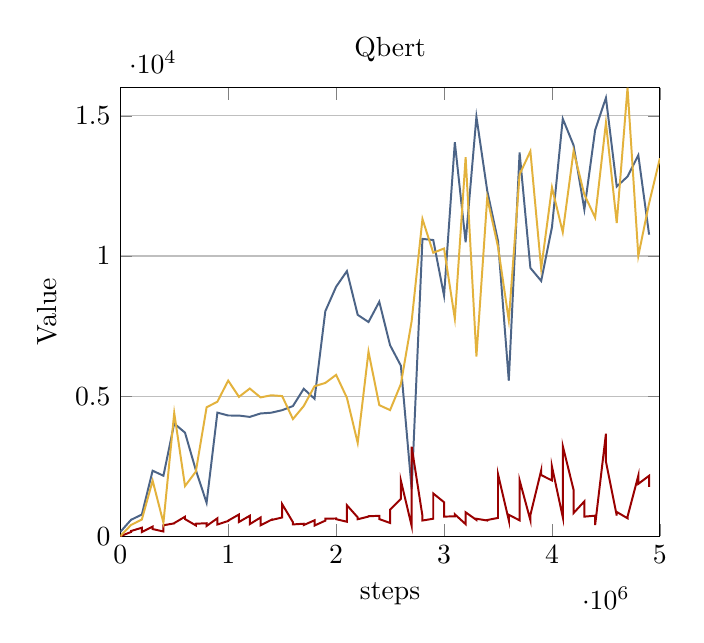
\begin{tikzpicture}

\begin{axis}[%
title=Qbert,
% %width=4.634in,
%width=10in,
%height=5in,
%at={(2.596in,2.358in)},
% scale only axis,
xmin=0,
xmax=5000000,
xlabel style={font=\color{white!15!black}},
xlabel={steps},
xlabel near ticks,
ymin=0,
ymax=16000,
ylabel style={font=\color{white!15!black}},
ylabel={Value},
ylabel near ticks,
ymajorgrids,
% %scale=0.5,
%scale=0.4,
axis background/.style={fill=white},
%legend style={legend cell align=left, align=left, draw=white!15!black}
]
\addplot [color=blue, line width = 0.25mm]
                table[row sep=crcr]{
                  0 150.0\\ 
100000 585.0\\ 
200000 772.5\\ 
300000 2337.5\\ 
400000 2157.5\\ 
500000 4022.5\\ 
600000 3695.0\\ 
700000 2362.5\\ 
800000 1192.5\\ 
900000 4410.0\\ 
1000000 4307.5\\ 
1100000 4305.0\\ 
1200000 4257.5\\ 
1300000 4380.0\\ 
1400000 4407.5\\ 
1500000 4497.5\\ 
1600000 4645.0\\ 
1700000 5260.0\\ 
1800000 4905.0\\ 
1900000 8030.0\\ 
2000000 8902.5\\ 
2100000 9460.0\\ 
2200000 7900.0\\ 
2300000 7642.5\\ 
2400000 8367.5\\ 
2500000 6815.0\\ 
2600000 6085.0\\ 
2700000 1677.5\\ 
2800000 10610.0\\ 
2900000 10570.0\\ 
3000000 8585.0\\ 
3100000 14057.5\\ 
3200000 10490.0\\ 
3300000 14970.0\\ 
3400000 12332.5\\ 
3500000 10537.5\\ 
3600000 5550.0\\ 
3700000 13692.5\\ 
3800000 9572.5\\ 
3900000 9110.0\\ 
4000000 11030.0\\ 
4100000 14897.5\\ 
4200000 13955.0\\ 
4300000 11660.0\\ 
4400000 14495.0\\ 
4500000 15645.0\\ 
4600000 12480.0\\ 
4700000 12835.0\\ 
4800000 13597.5\\ 
4900000 10762.5\\ 
};
\addplot [color=red, line width = 0.25mm]
                table[row sep=crcr]{
                  0 0.0\\ 
0 0.0\\ 
100000 150.0\\ 
100000 185.0\\ 
200000 302.5\\ 
200000 150.0\\ 
300000 342.5\\ 
300000 255.0\\ 
400000 167.5\\ 
400000 390.0\\ 
500000 457.5\\ 
500000 467.5\\ 
600000 695.0\\ 
600000 610.0\\ 
700000 385.0\\ 
700000 445.0\\ 
800000 462.5\\ 
800000 365.0\\ 
900000 640.0\\ 
900000 417.5\\ 
1000000 542.5\\ 
1000000 555.0\\ 
1100000 775.0\\ 
1100000 507.5\\ 
1200000 730.0\\ 
1200000 430.0\\ 
1300000 667.5\\ 
1300000 387.5\\ 
1400000 585.0\\ 
1400000 577.5\\ 
1500000 667.5\\ 
1500000 1145.0\\ 
1600000 500.0\\ 
1600000 420.0\\ 
1700000 445.0\\ 
1700000 397.5\\ 
1800000 567.5\\ 
1800000 380.0\\ 
1900000 555.0\\ 
1900000 625.0\\ 
2000000 632.5\\ 
2000000 607.5\\ 
2100000 515.0\\ 
2100000 1105.0\\ 
2200000 672.5\\ 
2200000 605.0\\ 
2300000 700.0\\ 
2300000 712.5\\ 
2400000 727.5\\ 
2400000 610.0\\ 
2500000 472.5\\ 
2500000 947.5\\ 
2600000 1330.0\\ 
2600000 1985.0\\ 
2700000 365.0\\ 
2700000 3195.0\\ 
2800000 720.0\\ 
2800000 560.0\\ 
2900000 622.5\\ 
2900000 1525.0\\ 
3000000 1212.5\\ 
3000000 700.0\\ 
3100000 707.5\\ 
3100000 780.0\\ 
3200000 430.0\\ 
3200000 852.5\\ 
3300000 580.0\\ 
3300000 622.5\\ 
3400000 560.0\\ 
3400000 577.5\\ 
3500000 652.5\\ 
3500000 2215.0\\ 
3600000 567.5\\ 
3600000 765.0\\ 
3700000 565.0\\ 
3700000 1995.0\\ 
3800000 570.0\\ 
3800000 757.5\\ 
3900000 2345.0\\ 
3900000 2182.5\\ 
4000000 1987.5\\ 
4000000 2482.5\\ 
4100000 682.5\\ 
4100000 3220.0\\ 
4200000 1657.5\\ 
4200000 825.0\\ 
4300000 1242.5\\ 
4300000 697.5\\ 
4400000 732.5\\ 
4400000 397.5\\ 
4500000 3660.0\\ 
4500000 2662.5\\ 
4600000 735.0\\ 
4600000 865.0\\ 
4700000 640.0\\ 
4700000 695.0\\ 
4800000 2160.0\\ 
4800000 1867.5\\ 
4900000 2157.5\\ 
4900000 1762.5\\ 
};
\addplot [color=yellow, line width = 0.25mm]
                table[row sep=crcr]{
                  0 0.0\\ 
0 0.0\\ 
0 0.0\\ 
0 0.0\\ 
100000 400.0\\ 
200000 595.0\\ 
300000 1982.5\\ 
400000 480.0\\ 
500000 4397.5\\ 
600000 1790.0\\ 
700000 2302.5\\ 
800000 4600.0\\ 
900000 4800.0\\ 
1000000 5552.5\\ 
1100000 4972.5\\ 
1200000 5270.0\\ 
1300000 4952.5\\ 
1400000 5030.0\\ 
1500000 5000.0\\ 
1600000 4180.0\\ 
1700000 4645.0\\ 
1800000 5352.5\\ 
1900000 5470.0\\ 
2000000 5757.5\\ 
2100000 4940.0\\ 
2200000 3327.5\\ 
2300000 6585.0\\ 
2400000 4677.5\\ 
2500000 4500.0\\ 
2600000 5430.0\\ 
2700000 7677.5\\ 
2800000 11320.0\\ 
2900000 10115.0\\ 
3000000 10267.5\\ 
3100000 7765.0\\ 
3200000 13525.0\\ 
3300000 6415.0\\ 
3400000 12077.5\\ 
3500000 10327.5\\ 
3600000 7700.0\\ 
3700000 12912.5\\ 
3800000 13737.5\\ 
3900000 9552.5\\ 
4000000 12445.0\\ 
4100000 10847.5\\ 
4200000 13737.5\\ 
4300000 12195.0\\ 
4400000 11370.0\\ 
4500000 14755.0\\ 
4600000 11175.0\\ 
4700000 16002.5\\ 
4800000 10005.0\\ 
4900000 11885.0\\ 
5000000 13490.0\\ 
};
\end{axis}
\end{tikzpicture}}}
    \subfloat[]{  \resizebox{0.4\textwidth}{!}{
\definecolor{blue}{RGB}{76,100,135}
\definecolor{red}{RGB}{153,0,0}
\definecolor{yellow}{RGB}{227,178,60}
\definecolor{mycolor1}{rgb}{0.00000,0.44700,0.74100}%
\definecolor{mycolor2}{rgb}{0.85000,0.32500,0.09800}%
\definecolor{mycolor3}{rgb}{0.92900,0.69400,0.12500}%
%
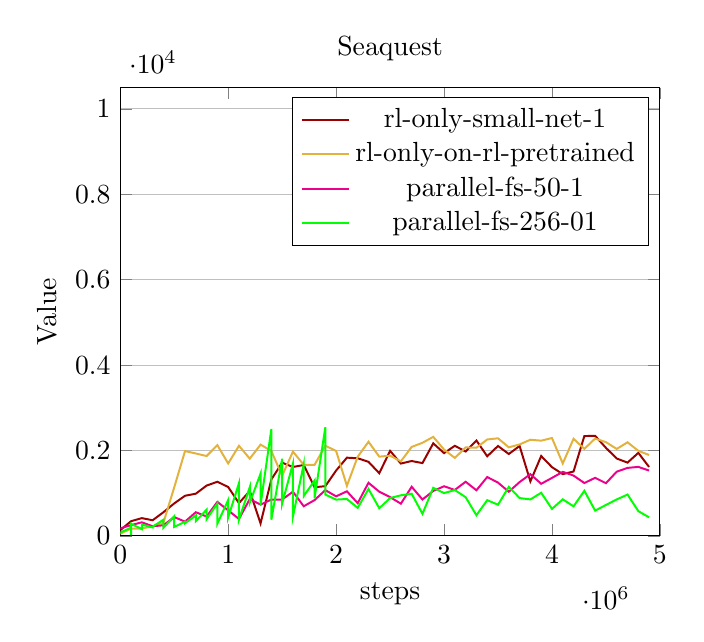
\begin{tikzpicture}

\begin{axis}[%
title=Seaquest,
% %width=4.634in,
%width=10in,
%height=5in,
%at={(2.596in,2.358in)},
% scale only axis,
xmin=0,
xmax=5000000,
xlabel style={font=\color{white!15!black}},
xlabel={steps},
xlabel near ticks,
ymin=0,
ymax=10500,
ylabel style={font=\color{white!15!black}},
ylabel={Value},
ylabel near ticks,
ymajorgrids,
% %scale=0.5,
%scale=0.4,
axis background/.style={fill=white},
%legend style={legend cell align=left, align=left, draw=white!15!black}
]
\addplot [color=red, line width = 0.25mm]
                table[row sep=crcr]{
                  0 134.0\\ 
100000 344.0\\ 
200000 416.0\\ 
300000 366.0\\ 
400000 554.0\\ 
500000 760.0\\ 
600000 940.0\\ 
700000 988.0\\ 
800000 1178.0\\ 
900000 1268.0\\ 
1000000 1144.0\\ 
1100000 768.0\\ 
1200000 1052.0\\ 
1300000 292.0\\ 
1400000 1322.0\\ 
1500000 1714.0\\ 
1600000 1614.0\\ 
1700000 1660.0\\ 
1800000 1140.0\\ 
1900000 1164.0\\ 
2000000 1530.0\\ 
2100000 1832.0\\ 
2200000 1818.0\\ 
2300000 1734.0\\ 
2400000 1468.0\\ 
2500000 1992.0\\ 
2600000 1694.0\\ 
2700000 1754.0\\ 
2800000 1704.0\\ 
2900000 2168.0\\ 
3000000 1938.0\\ 
3100000 2110.0\\ 
3200000 1976.0\\ 
3300000 2234.0\\ 
3400000 1864.0\\ 
3500000 2106.0\\ 
3600000 1918.0\\ 
3700000 2106.0\\ 
3800000 1276.0\\ 
3900000 1870.0\\ 
4000000 1610.0\\ 
4100000 1446.0\\ 
4200000 1508.0\\ 
4300000 2338.0\\ 
4400000 2344.0\\ 
4500000 2062.0\\ 
4600000 1812.0\\ 
4700000 1716.0\\ 
4800000 1944.0\\ 
4900000 1614.0\\ 
};
\addlegendentry{rl-only-small-net-1}
\addplot [color=yellow, line width = 0.25mm]
                table[row sep=crcr]{
                  0 48.0\\ 
100000 172.0\\ 
200000 172.0\\ 
300000 224.0\\ 
400000 308.0\\ 
500000 1136.0\\ 
600000 1986.0\\ 
700000 1930.0\\ 
800000 1870.0\\ 
900000 2124.0\\ 
1000000 1696.0\\ 
1100000 2110.0\\ 
1200000 1808.0\\ 
1300000 2138.0\\ 
1400000 1988.0\\ 
1500000 1408.0\\ 
1600000 1974.0\\ 
1700000 1664.0\\ 
1800000 1662.0\\ 
1900000 2112.0\\ 
2000000 1990.0\\ 
2100000 1172.0\\ 
2200000 1854.0\\ 
2300000 2204.0\\ 
2400000 1856.0\\ 
2500000 1878.0\\ 
2600000 1746.0\\ 
2700000 2084.0\\ 
2800000 2180.0\\ 
2900000 2320.0\\ 
3000000 2022.0\\ 
3100000 1826.0\\ 
3200000 2072.0\\ 
3300000 2064.0\\ 
3400000 2258.0\\ 
3500000 2286.0\\ 
3600000 2074.0\\ 
3700000 2142.0\\ 
3800000 2252.0\\ 
3900000 2230.0\\ 
4000000 2292.0\\ 
4100000 1696.0\\ 
4200000 2274.0\\ 
4300000 2038.0\\ 
4400000 2280.0\\ 
4500000 2196.0\\ 
4600000 2036.0\\ 
4700000 2192.0\\ 
4800000 1992.0\\ 
4900000 1894.0\\ 
};
\addlegendentry{rl-only-on-rl-pretrained}
\addplot [color=magenta, line width = 0.25mm]
                table[row sep=crcr]{
                  0 176.0\\ 
0 176.0\\ 
100000 252.0\\ 
200000 318.0\\ 
300000 226.0\\ 
400000 248.0\\ 
500000 440.0\\ 
600000 334.0\\ 
700000 554.0\\ 
800000 454.0\\ 
900000 796.0\\ 
1000000 598.0\\ 
1100000 396.0\\ 
1200000 862.0\\ 
1300000 732.0\\ 
1400000 850.0\\ 
1500000 852.0\\ 
1600000 1034.0\\ 
1700000 694.0\\ 
1800000 838.0\\ 
1900000 1072.0\\ 
2000000 926.0\\ 
2100000 1044.0\\ 
2200000 766.0\\ 
2300000 1244.0\\ 
2400000 1034.0\\ 
2500000 908.0\\ 
2600000 754.0\\ 
2700000 1150.0\\ 
2800000 852.0\\ 
2900000 1052.0\\ 
3000000 1162.0\\ 
3100000 1076.0\\ 
3200000 1268.0\\ 
3300000 1068.0\\ 
3400000 1378.0\\ 
3500000 1248.0\\ 
3600000 1034.0\\ 
3700000 1260.0\\ 
3800000 1446.0\\ 
3900000 1220.0\\ 
4000000 1358.0\\ 
4100000 1500.0\\ 
4200000 1412.0\\ 
4300000 1238.0\\ 
4400000 1360.0\\ 
4500000 1234.0\\ 
4600000 1504.0\\ 
4700000 1592.0\\ 
4800000 1616.0\\ 
4900000 1530.0\\ 
};
\addlegendentry{parallel-fs-50-1}
\addplot [color=green, line width = 0.25mm]
                table[row sep=crcr]{
                  0 80.0\\ 
0 80.0\\ 
0 80.0\\ 
100000 192.0\\ 
100000 20.0\\ 
100000 284.0\\ 
200000 158.0\\ 
200000 264.0\\ 
300000 198.0\\ 
300000 216.0\\ 
400000 378.0\\ 
400000 192.0\\ 
500000 460.0\\ 
500000 210.0\\ 
600000 330.0\\ 
600000 296.0\\ 
700000 478.0\\ 
700000 344.0\\ 
800000 614.0\\ 
800000 390.0\\ 
900000 758.0\\ 
900000 288.0\\ 
1000000 840.0\\ 
1000000 432.0\\ 
1100000 1236.0\\ 
1100000 384.0\\ 
1200000 1142.0\\ 
1200000 776.0\\ 
1300000 1458.0\\ 
1300000 730.0\\ 
1400000 2504.0\\ 
1400000 380.0\\ 
1500000 1806.0\\ 
1500000 756.0\\ 
1600000 1695.0\\ 
1600000 454.0\\ 
1700000 1678.0\\ 
1700000 932.0\\ 
1800000 1296.0\\ 
1800000 878.0\\ 
1900000 2544.0\\ 
1900000 968.0\\ 
2000000 850.0\\ 
2100000 864.0\\ 
2200000 656.0\\ 
2300000 1098.0\\ 
2400000 648.0\\ 
2500000 886.0\\ 
2600000 950.0\\ 
2700000 988.0\\ 
2800000 516.0\\ 
2900000 1126.0\\ 
3000000 1002.0\\ 
3100000 1074.0\\ 
3200000 906.0\\ 
3300000 484.0\\ 
3400000 836.0\\ 
3500000 730.0\\ 
3600000 1148.0\\ 
3700000 886.0\\ 
3800000 854.0\\ 
3900000 1010.0\\ 
4000000 632.0\\ 
4100000 856.0\\ 
4200000 692.0\\ 
4300000 1056.0\\ 
4400000 592.0\\ 
4500000 724.0\\ 
4600000 854.0\\ 
4700000 968.0\\ 
4800000 580.0\\ 
4900000 434.0\\ 
};
\addlegendentry{parallel-fs-256-01}
\end{axis}
\end{tikzpicture}}}\\
  \vspace{-1cm}
    \subfloat[]{  \resizebox{0.4\textwidth}{!}{
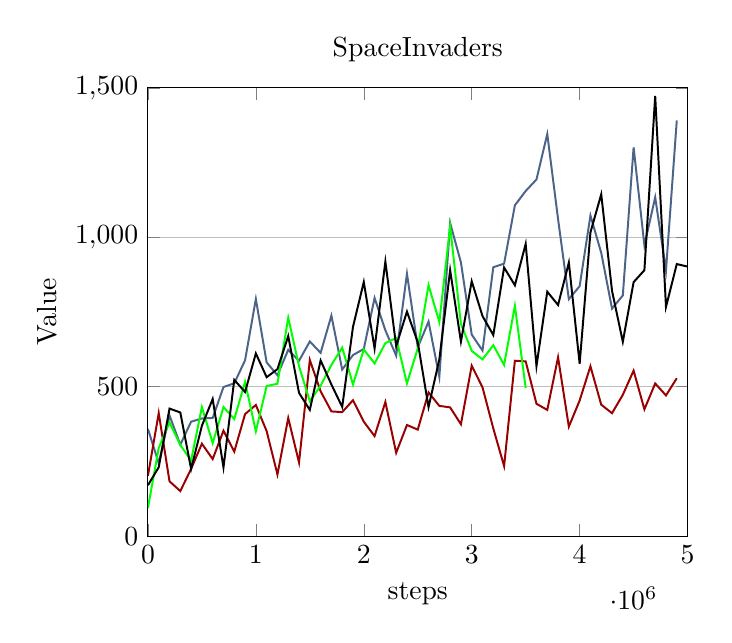
\begin{tikzpicture}

\begin{axis}[%
title=SpaceInvaders,
%width=10in,
%height=5in,
%at={(2.596in,2.358in)},
% scale only axis,
xmin=0,
xmax=5000000,
xlabel style={font=\color{white!15!black}},
xlabel={steps},
xlabel near ticks,
ymin=0,
ymax=1500,
ylabel style={font=\color{white!15!black}},
ylabel={Value},
ylabel near ticks,
ymajorgrids,
% %scale=0.5,
%scale=0.4,
axis background/.style={fill=white},
%legend style={legend cell align=left, align=left, draw=white!15!black}
]
\addplot [color=blue, line width = 0.25mm]
                table[row sep=crcr]{
                  0 359.0\\ 
100000 244.0\\ 
200000 404.0\\ 
300000 306.0\\ 
400000 383.0\\ 
500000 394.0\\ 
600000 395.5\\ 
700000 499.0\\ 
800000 511.5\\ 
900000 588.5\\ 
1000000 793.5\\ 
1100000 581.5\\ 
1200000 538.5\\ 
1300000 623.5\\ 
1400000 587.0\\ 
1500000 651.5\\ 
1600000 613.5\\ 
1700000 738.0\\ 
1800000 557.5\\ 
1900000 606.0\\ 
2000000 626.5\\ 
2100000 797.0\\ 
2200000 689.0\\ 
2300000 604.0\\ 
2400000 878.0\\ 
2500000 632.0\\ 
2600000 718.0\\ 
2700000 533.0\\ 
2800000 1048.0\\ 
2900000 916.0\\ 
3000000 674.5\\ 
3100000 621.0\\ 
3200000 900.0\\ 
3300000 912.0\\ 
3400000 1107.0\\ 
3500000 1155.0\\ 
3600000 1193.5\\ 
3700000 1345.5\\ 
3800000 1061.0\\ 
3900000 793.0\\ 
4000000 836.5\\ 
4100000 1073.0\\ 
4200000 948.0\\ 
4300000 761.5\\ 
4400000 805.5\\ 
4500000 1301.0\\ 
4600000 973.0\\ 
4700000 1134.0\\ 
4800000 889.5\\ 
4900000 1391.0\\ 
};
\addplot [color=red, line width = 0.25mm]
                table[row sep=crcr]{
                  0 202.0\\ 
100000 412.0\\ 
200000 183.5\\ 
300000 151.0\\ 
400000 225.0\\ 
500000 309.5\\ 
600000 258.0\\ 
700000 353.0\\ 
800000 283.0\\ 
900000 408.5\\ 
1000000 439.0\\ 
1100000 351.5\\ 
1200000 206.5\\ 
1300000 395.5\\ 
1400000 246.5\\ 
1500000 589.5\\ 
1600000 485.0\\ 
1700000 417.5\\ 
1800000 415.0\\ 
1900000 455.0\\ 
2000000 383.0\\ 
2100000 335.0\\ 
2200000 449.0\\ 
2300000 279.0\\ 
2400000 372.0\\ 
2500000 356.5\\ 
2600000 481.0\\ 
2700000 436.0\\ 
2800000 431.0\\ 
2900000 374.5\\ 
3000000 570.5\\ 
3100000 498.0\\ 
3200000 360.5\\ 
3300000 234.5\\ 
3400000 587.0\\ 
3500000 585.0\\ 
3600000 443.0\\ 
3700000 422.5\\ 
3800000 598.5\\ 
3900000 366.5\\ 
4000000 454.0\\ 
4100000 568.5\\ 
4200000 440.0\\ 
4300000 411.5\\ 
4400000 473.0\\ 
4500000 554.0\\ 
4600000 424.5\\ 
4700000 511.0\\ 
4800000 471.0\\ 
4900000 528.5\\ 
};
\addplot [color=green, line width = 0.25mm]
                table[row sep=crcr]{
                  0 94.5\\ 
100000 295.0\\ 
200000 380.5\\ 
300000 305.0\\ 
400000 253.0\\ 
500000 432.0\\ 
600000 311.5\\ 
700000 432.0\\ 
800000 392.0\\ 
900000 516.0\\ 
1000000 351.0\\ 
1100000 502.5\\ 
1200000 510.0\\ 
1300000 731.0\\ 
1400000 569.0\\ 
1500000 451.5\\ 
1600000 503.5\\ 
1700000 573.0\\ 
1800000 631.0\\ 
1900000 507.5\\ 
2000000 624.5\\ 
2100000 578.0\\ 
2200000 646.0\\ 
2300000 663.0\\ 
2400000 511.0\\ 
2500000 628.0\\ 
2600000 840.0\\ 
2700000 716.5\\ 
2800000 1037.0\\ 
2900000 710.5\\ 
3000000 620.0\\ 
3100000 591.5\\ 
3200000 639.0\\ 
3300000 573.0\\ 
3400000 771.0\\ 
3500000 496.0\\ 
};
\addplot [color=black, line width = 0.25mm]
                table[row sep=crcr]{
                  0 170.5\\ 
100000 230.5\\ 
200000 427.0\\ 
300000 414.0\\ 
400000 225.0\\ 
500000 369.5\\ 
600000 459.0\\ 
700000 230.0\\ 
800000 523.0\\ 
900000 482.5\\ 
1000000 611.5\\ 
1100000 532.0\\ 
1200000 559.0\\ 
1300000 669.5\\ 
1400000 479.5\\ 
1500000 422.5\\ 
1600000 588.0\\ 
1700000 507.5\\ 
1800000 432.5\\ 
1900000 700.5\\ 
2000000 850.5\\ 
2100000 628.0\\ 
2200000 919.0\\ 
2300000 636.0\\ 
2400000 751.5\\ 
2500000 649.0\\ 
2600000 432.0\\ 
2700000 591.5\\ 
2800000 890.0\\ 
2900000 651.0\\ 
3000000 853.0\\ 
3100000 736.5\\ 
3200000 673.0\\ 
3300000 899.0\\ 
3400000 839.5\\ 
3500000 978.0\\ 
3600000 569.0\\ 
3700000 818.0\\ 
3800000 773.5\\ 
3900000 915.5\\ 
4000000 577.0\\ 
4100000 1016.5\\ 
4200000 1144.0\\ 
4300000 821.0\\ 
4400000 650.5\\ 
4500000 850.0\\ 
4600000 890.0\\ 
4700000 1473.0\\ 
4800000 767.0\\ 
4900000 910.5\\ 
5000000 902.0\\ 
};
\end{axis}
\end{tikzpicture}}}
  \\

  \ref{named}
  \caption{Effectiveness of parallel training. Overall the results are negative, some slightly
  and others strongly. Interestingly, using a pretrained encoder has a negative effect
in this case. We suspect that this is due to the fixation on a particular local minimum caused
by reconstruction loss. Importantly, the negative effect is present despite
regularization maintaining a fixed latent space over a relatively large number of epochs (5-10).
Results tend to be worse in games where MSE loss is less suitable and in games
with larger visual complexity.}
  \label{fig-parallel}
\end{figure}

\section{Effectiveness of regularization}
\label{sec-effectiveness-of-reg}
Before continuing the discussion, the effectiveness of regularization needs to be discussed.
We present runs with both data augmentation and L2 regularization, runs with either one or the other and
runs without neither in \ref{fig:reg-vs-no-reg}.

\begin{figure}[!t]
  \captionsetup[subfloat]{position=top,labelformat=empty}
  \vspace{-1.5cm}
  \centering

    \subfloat[]{  \resizebox{0.4\textwidth}{!}{
%\definecolor{blue}{RGB}{76,100,135}
%\definecolor{red}{RGB}{153,0,0}
%\definecolor{yellow}{RGB}{227,178,60}
%\definecolor{mycolor1}{rgb}{0.00000,0.44700,0.74100}%
%\definecolor{mycolor2}{rgb}{0.85000,0.32500,0.09800}%
%\definecolor{mycolor3}{rgb}{0.92900,0.69400,0.12500}%
%
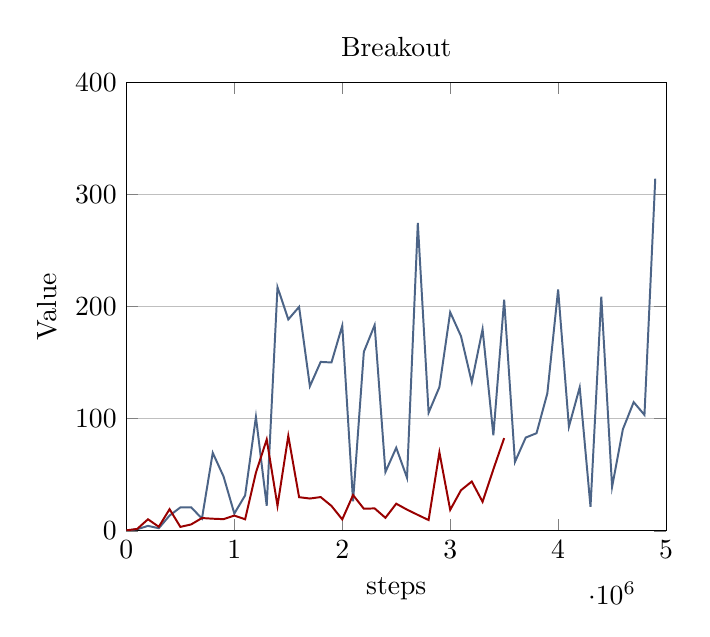
\begin{tikzpicture}

\begin{axis}[%
legend entries={rl-only-small-net,L2-reg,parallel-fs-50-no-aug}, 
legend columns=2,
title=Breakout,
legend to name=named,
legend style={legend cell align=left},
%%width=10in,
%%height=5in,
%%at={(2.596in,2.358in)},
% scale only axis,
xmin=0,
xmax=5000000,
xlabel style={font=\color{white!15!black}},
xlabel={steps},
xlabel near ticks,
ymin=0,
ymax=400,
ylabel style={font=\color{white!15!black}},
ylabel={Value},
ylabel near ticks,
ymajorgrids,
% %scale=0.5,
%%scale=0.4,
axis background/.style={fill=white},
%legend columns=2,
%legend=south outside
]
\addplot [color=blue, line width = 0.25mm]
                table[row sep=crcr]{
                  0 0.20000000298023224\\ 
100000 1.399999976158142\\ 
200000 4.400000095367432\\ 
300000 2.299999952316284\\ 
400000 13.600000381469727\\ 
500000 20.899999618530273\\ 
600000 21.0\\ 
700000 10.899999618530273\\ 
800000 69.5999984741211\\ 
900000 48.5\\ 
1000000 15.399999618530273\\ 
1100000 31.600000381469727\\ 
1200000 101.5999984741211\\ 
1300000 22.399999618530273\\ 
1400000 217.39999389648438\\ 
1500000 188.60000610351562\\ 
1600000 199.8000030517578\\ 
1700000 129.0\\ 
1800000 150.6999969482422\\ 
1900000 150.1999969482422\\ 
2000000 183.0\\ 
2100000 26.399999618530273\\ 
2200000 159.6999969482422\\ 
2300000 183.5\\ 
2400000 52.5\\ 
2500000 74.0999984741211\\ 
2600000 47.29999923706055\\ 
2700000 274.6000061035156\\ 
2800000 105.4000015258789\\ 
2900000 128.1999969482422\\ 
3000000 195.0\\ 
3100000 173.6999969482422\\ 
3200000 132.60000610351562\\ 
3300000 179.89999389648438\\ 
3400000 85.19999694824219\\ 
3500000 206.1999969482422\\ 
3600000 61.5\\ 
3700000 83.19999694824219\\ 
3800000 87.0999984741211\\ 
3900000 122.5999984741211\\ 
4000000 215.3000030517578\\ 
4100000 92.9000015258789\\ 
4200000 128.0\\ 
4300000 21.399999618530273\\ 
4400000 208.89999389648438\\ 
4500000 39.20000076293945\\ 
4600000 90.5999984741211\\ 
4700000 114.80000305175781\\ 
4800000 103.4000015258789\\ 
4900000 314.20001220703125\\ 
};
\addplot [color=red, line width = 0.25mm]
                table[row sep=crcr]{
                  0 0.4000000059604645\\ 
100000 1.7000000476837158\\ 
200000 10.300000190734863\\ 
300000 3.5999999046325684\\ 
400000 19.299999237060547\\ 
500000 3.5\\ 
600000 5.699999809265137\\ 
700000 11.399999618530273\\ 
800000 10.800000190734863\\ 
900000 10.399999618530273\\ 
1000000 13.600000381469727\\ 
1100000 10.300000190734863\\ 
1200000 51.900001525878906\\ 
1300000 81.5\\ 
1400000 22.299999237060547\\ 
1500000 84.69999694824219\\ 
1600000 30.0\\ 
1700000 28.799999237060547\\ 
1800000 30.100000381469727\\ 
1900000 22.200000762939453\\ 
2000000 10.199999809265137\\ 
2100000 31.899999618530273\\ 
2200000 19.700000762939453\\ 
2300000 20.0\\ 
2400000 11.600000381469727\\ 
2500000 24.200000762939453\\ 
2600000 18.899999618530273\\ 
2700000 14.199999809265137\\ 
2800000 9.600000381469727\\ 
2900000 70.0\\ 
3000000 18.700000762939453\\ 
3100000 36.20000076293945\\ 
3200000 44.0\\ 
3300000 25.899999618530273\\ 
3400000 54.900001525878906\\ 
3500000 82.69999694824219\\ 
};
\addplot [color=yellow, line width = 0.25mm]
                table[row sep=crcr]{
                  0 0.800000011920929\\ 
};
\end{axis}
\end{tikzpicture}}}
    \subfloat[]{  \resizebox{0.4\textwidth}{!}{
%\definecolor{blue}{RGB}{76,100,135}
%\definecolor{red}{RGB}{153,0,0}
%\definecolor{yellow}{RGB}{227,178,60}
%\definecolor{mycolor1}{rgb}{0.00000,0.44700,0.74100}%
%\definecolor{mycolor2}{rgb}{0.85000,0.32500,0.09800}%
%\definecolor{mycolor3}{rgb}{0.92900,0.69400,0.12500}%
%
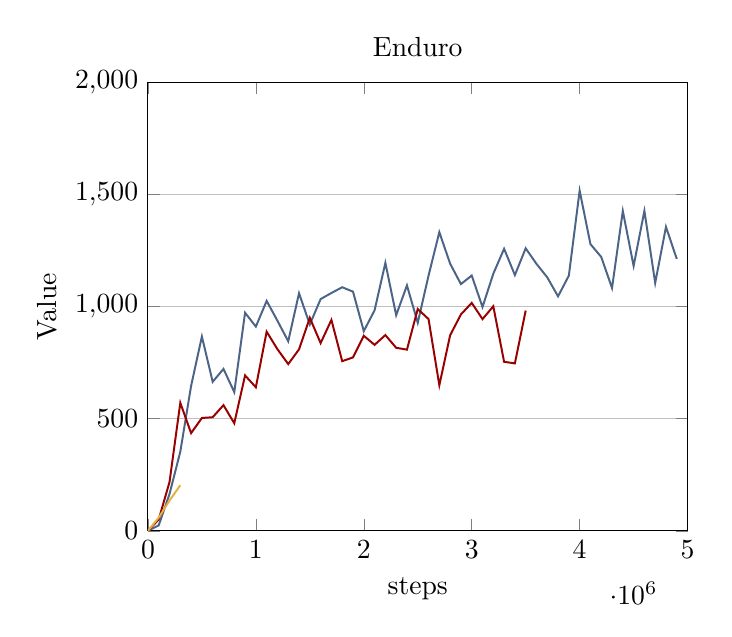
\begin{tikzpicture}

\begin{axis}[%
title=Enduro,
% %width=4.634in,
%%width=10in,
%%height=5in,
%at={(2.596in,2.358in)},
% scale only axis,
xmin=0,
xmax=5000000,
xlabel style={font=\color{white!15!black}},
xlabel={steps},
xlabel near ticks,
ymin=0,
ymax=2000,
ylabel style={font=\color{white!15!black}},
ylabel={Value},
ylabel near ticks,
ymajorgrids,
% %scale=0.5,
%scale=0.4,
axis background/.style={fill=white},
%legend style={legend cell align=left, align=left, draw=white!15!black}
]
\addplot [color=blue, line width = 0.25mm]
                table[row sep=crcr]{
                  0 0.0\\ 
100000 24.299999237060547\\ 
200000 164.3000030517578\\ 
300000 353.0\\ 
400000 646.4000244140625\\ 
500000 866.7000122070312\\ 
600000 664.7000122070312\\ 
700000 722.2000122070312\\ 
800000 618.9000244140625\\ 
900000 972.7999877929688\\ 
1000000 910.9000244140625\\ 
1100000 1025.699951171875\\ 
1200000 937.0\\ 
1300000 845.5999755859375\\ 
1400000 1059.9000244140625\\ 
1500000 920.2999877929688\\ 
1600000 1033.800048828125\\ 
1700000 1061.0\\ 
1800000 1086.5999755859375\\ 
1900000 1066.9000244140625\\ 
2000000 890.9000244140625\\ 
2100000 983.5\\ 
2200000 1195.300048828125\\ 
2300000 962.0\\ 
2400000 1094.800048828125\\ 
2500000 928.0\\ 
2600000 1138.5999755859375\\ 
2700000 1332.300048828125\\ 
2800000 1191.800048828125\\ 
2900000 1100.5999755859375\\ 
3000000 1138.800048828125\\ 
3100000 998.2999877929688\\ 
3200000 1146.800048828125\\ 
3300000 1258.0999755859375\\ 
3400000 1141.0\\ 
3500000 1260.300048828125\\ 
3600000 1190.800048828125\\ 
3700000 1130.5999755859375\\ 
3800000 1046.0999755859375\\ 
3900000 1138.4000244140625\\ 
4000000 1517.5\\ 
4100000 1278.9000244140625\\ 
4200000 1221.699951171875\\ 
4300000 1083.199951171875\\ 
4400000 1426.9000244140625\\ 
4500000 1181.5999755859375\\ 
4600000 1427.199951171875\\ 
4700000 1105.800048828125\\ 
4800000 1355.800048828125\\ 
4900000 1212.9000244140625\\ 
};
\addplot [color=red, line width = 0.25mm]
                table[row sep=crcr]{
                  0 0.0\\ 
100000 50.5\\ 
200000 217.60000610351562\\ 
300000 570.9000244140625\\ 
400000 435.6000061035156\\ 
500000 503.3999938964844\\ 
600000 506.79998779296875\\ 
700000 560.5\\ 
800000 479.79998779296875\\ 
900000 693.2000122070312\\ 
1000000 640.4000244140625\\ 
1100000 888.4000244140625\\ 
1200000 810.0999755859375\\ 
1300000 743.7999877929688\\ 
1400000 809.5\\ 
1500000 950.2000122070312\\ 
1600000 837.4000244140625\\ 
1700000 940.7999877929688\\ 
1800000 756.7999877929688\\ 
1900000 773.5\\ 
2000000 870.0999755859375\\ 
2100000 829.5999755859375\\ 
2200000 873.2000122070312\\ 
2300000 816.5\\ 
2400000 808.2000122070312\\ 
2500000 989.5999755859375\\ 
2600000 944.5\\ 
2700000 649.4000244140625\\ 
2800000 872.4000244140625\\ 
2900000 965.2000122070312\\ 
3000000 1016.7000122070312\\ 
3100000 944.4000244140625\\ 
3200000 1001.7000122070312\\ 
3300000 754.0\\ 
3400000 746.7999877929688\\ 
3500000 982.2999877929688\\ 
};
\addplot [color=yellow, line width = 0.25mm]
                table[row sep=crcr]{
                  0 0.0\\ 
100000 58.79999923706055\\ 
200000 135.10000610351562\\ 
300000 203.1999969482422\\ 
};
\end{axis}
\end{tikzpicture}}}\\
  \vspace{-1cm}
    \subfloat[]{  \resizebox{0.4\textwidth}{!}{
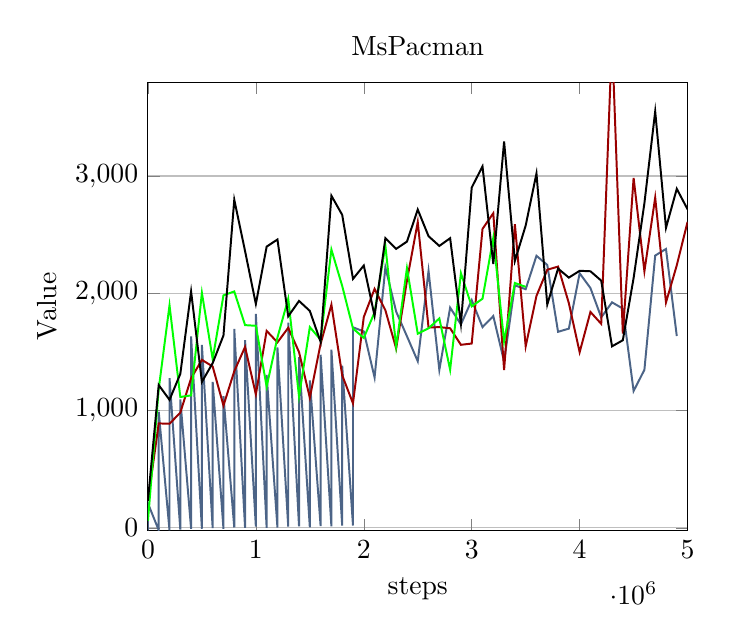
\begin{tikzpicture}

\begin{axis}[%
title=MsPacman,
% %width=4.634in,
%width=10in,
%height=5in,
%at={(2.596in,2.358in)},
% scale only axis,
xmin=0,
xmax=5000000,
xlabel style={font=\color{white!15!black}},
xlabel={steps},
xlabel near ticks,
ymin=-22,
ymax=3800,
ylabel style={font=\color{white!15!black}},
ylabel={Value},
ylabel near ticks,
ymajorgrids,
% %scale=0.5,
%scale=0.4,
axis background/.style={fill=white},
%legend style={legend cell align=left, align=left, draw=white!15!black}
]
\addplot [color=blue, line width = 0.25mm]
                table[row sep=crcr]{
                  0 -21.0\\ 
0 210.0\\ 
100000 -19.799999237060547\\ 
100000 990.0\\ 
200000 -20.700000762939453\\ 
200000 1277.0\\ 
300000 -15.0\\ 
300000 1096.0\\ 
400000 -7.0\\ 
400000 1632.0\\ 
500000 -6.900000095367432\\ 
500000 1561.0\\ 
600000 -1.899999976158142\\ 
600000 1245.0\\ 
700000 -7.599999904632568\\ 
700000 1123.0\\ 
800000 4.0\\ 
800000 1696.0\\ 
900000 1.5\\ 
900000 1600.0\\ 
1000000 11.300000190734863\\ 
1000000 1824.0\\ 
1100000 1.2000000476837158\\ 
1100000 1304.0\\ 
1200000 3.700000047683716\\ 
1200000 1538.0\\ 
1300000 11.5\\ 
1300000 1750.0\\ 
1400000 13.600000381469727\\ 
1400000 1456.0\\ 
1500000 5.699999809265137\\ 
1500000 1258.0\\ 
1600000 15.600000381469727\\ 
1600000 1476.0\\ 
1700000 13.5\\ 
1700000 1519.0\\ 
1800000 19.299999237060547\\ 
1800000 1383.0\\ 
1900000 20.799999237060547\\ 
1900000 1710.0\\ 
2000000 1675.0\\ 
2100000 1282.0\\ 
2200000 2222.0\\ 
2300000 1844.0\\ 
2400000 1634.0\\ 
2500000 1421.0\\ 
2600000 2191.0\\ 
2700000 1347.0\\ 
2800000 1878.0\\ 
2900000 1735.0\\ 
3000000 1942.0\\ 
3100000 1712.0\\ 
3200000 1806.0\\ 
3300000 1419.0\\ 
3400000 2068.0\\ 
3500000 2035.0\\ 
3600000 2320.0\\ 
3700000 2242.0\\ 
3800000 1672.0\\ 
3900000 1699.0\\ 
4000000 2171.0\\ 
4100000 2045.0\\ 
4200000 1795.0\\ 
4300000 1923.0\\ 
4400000 1870.0\\ 
4500000 1167.0\\ 
4600000 1348.0\\ 
4700000 2322.0\\ 
4800000 2378.0\\ 
4900000 1636.0\\ 
};
\addplot [color=red, line width = 0.25mm]
                table[row sep=crcr]{
                  0 230.0\\ 
100000 891.0\\ 
200000 888.0\\ 
300000 983.0\\ 
400000 1276.0\\ 
500000 1433.0\\ 
600000 1376.0\\ 
700000 1043.0\\ 
800000 1336.0\\ 
900000 1543.0\\ 
1000000 1139.0\\ 
1100000 1680.0\\ 
1200000 1582.0\\ 
1300000 1706.0\\ 
1400000 1499.0\\ 
1500000 1110.0\\ 
1600000 1569.0\\ 
1700000 1903.0\\ 
1800000 1301.0\\ 
1900000 1062.0\\ 
2000000 1798.0\\ 
2100000 2038.0\\ 
2200000 1856.0\\ 
2300000 1530.0\\ 
2400000 2109.0\\ 
2500000 2607.0\\ 
2600000 1708.0\\ 
2700000 1712.0\\ 
2800000 1702.0\\ 
2900000 1561.0\\ 
3000000 1572.0\\ 
3100000 2549.0\\ 
3200000 2683.0\\ 
3300000 1346.0\\ 
3400000 2590.0\\ 
3500000 1548.0\\ 
3600000 1978.0\\ 
3700000 2201.0\\ 
3800000 2228.0\\ 
3900000 1916.0\\ 
4000000 1498.0\\ 
4100000 1841.0\\ 
4200000 1740.0\\ 
4300000 4177.0\\ 
4400000 1656.0\\ 
4500000 2984.0\\ 
4600000 2188.0\\ 
4700000 2816.0\\ 
4800000 1922.0\\ 
4900000 2239.0\\ 
5000000 2609.0\\ 
};
\addplot [color=green, line width = 0.25mm]
                table[row sep=crcr]{
                  0 60.0\\ 
100000 1185.0\\ 
200000 1898.0\\ 
300000 1116.0\\ 
400000 1130.0\\ 
500000 2004.0\\ 
600000 1439.0\\ 
700000 1983.0\\ 
800000 2016.0\\ 
900000 1729.0\\ 
1000000 1723.0\\ 
1100000 1205.0\\ 
1200000 1623.0\\ 
1300000 1954.0\\ 
1400000 1121.0\\ 
1500000 1712.0\\ 
1600000 1604.0\\ 
1700000 2373.0\\ 
1800000 2063.0\\ 
1900000 1700.0\\ 
2000000 1620.0\\ 
2100000 1838.0\\ 
2200000 2406.0\\ 
2300000 1546.0\\ 
2400000 2215.0\\ 
2500000 1656.0\\ 
2600000 1702.0\\ 
2700000 1786.0\\ 
2800000 1348.0\\ 
2900000 2172.0\\ 
3000000 1889.0\\ 
3100000 1954.0\\ 
3200000 2473.0\\ 
3300000 1591.0\\ 
3400000 2088.0\\ 
3500000 2055.0\\ 
};
\addplot [color=black, line width = 0.25mm]
                table[row sep=crcr]{
                  0 230.0\\ 
100000 1218.0\\ 
200000 1092.0\\ 
300000 1313.0\\ 
400000 2016.0\\ 
500000 1245.0\\ 
600000 1405.0\\ 
700000 1641.0\\ 
800000 2798.0\\ 
900000 2360.0\\ 
1000000 1909.0\\ 
1100000 2398.0\\ 
1200000 2459.0\\ 
1300000 1804.0\\ 
1400000 1935.0\\ 
1500000 1850.0\\ 
1600000 1586.0\\ 
1700000 2832.0\\ 
1800000 2669.0\\ 
1900000 2123.0\\ 
2000000 2237.0\\ 
2100000 1808.0\\ 
2200000 2470.0\\ 
2300000 2379.0\\ 
2400000 2441.0\\ 
2500000 2714.0\\ 
2600000 2487.0\\ 
2700000 2404.0\\ 
2800000 2470.0\\ 
2900000 1739.0\\ 
3000000 2902.0\\ 
3100000 3082.0\\ 
3200000 2250.0\\ 
3300000 3294.0\\ 
3400000 2276.0\\ 
3500000 2578.0\\ 
3600000 3022.0\\ 
3700000 1904.0\\ 
3800000 2211.0\\ 
3900000 2134.0\\ 
4000000 2192.0\\ 
4100000 2188.0\\ 
4200000 2108.0\\ 
4300000 1548.0\\ 
4400000 1600.0\\ 
4500000 2130.0\\ 
4600000 2768.0\\ 
4700000 3551.0\\ 
4800000 2558.0\\ 
4900000 2891.0\\ 
5000000 2716.0\\ 
};
\end{axis}
\end{tikzpicture}}}
    \subfloat[]{  \resizebox{0.4\textwidth}{!}{
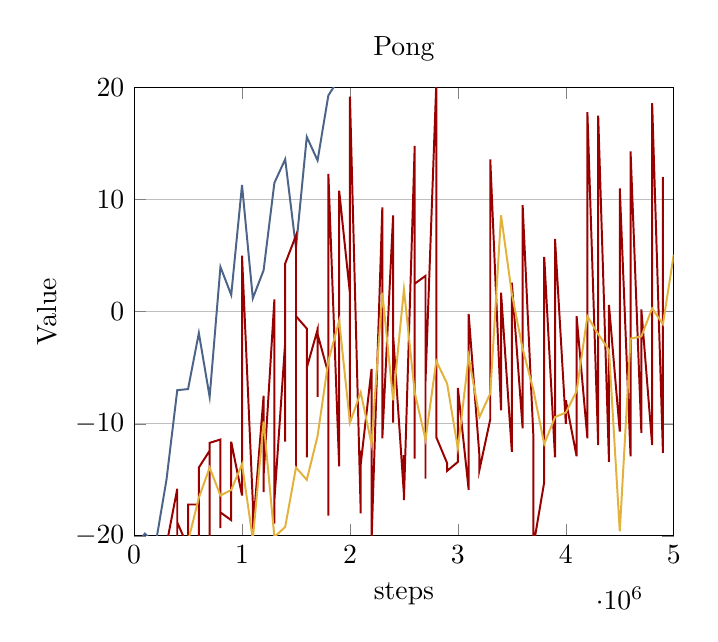
\begin{tikzpicture}

\begin{axis}[%
title=Pong,
% %width=4.634in,
%width=10in,
%height=5in,
%at={(2.596in,2.358in)},
% scale only axis,
xmin=0,
xmax=5000000,
xlabel style={font=\color{white!15!black}},
xlabel={steps},
xlabel near ticks,
ymin=-20,
ymax=20,
ylabel style={font=\color{white!15!black}},
ylabel={Value},
ylabel near ticks,
ymajorgrids,
% %scale=0.5,
%scale=0.4,
axis background/.style={fill=white},
%legend style={legend cell align=left, align=left, draw=white!15!black}
]
\addplot [color=blue, line width = 0.25mm]
                table[row sep=crcr]{
                  0 -21.0\\ 
100000 -19.799999237060547\\ 
200000 -20.700000762939453\\ 
300000 -15.0\\ 
400000 -7.0\\ 
500000 -6.900000095367432\\ 
600000 -1.899999976158142\\ 
700000 -7.599999904632568\\ 
800000 4.0\\ 
900000 1.5\\ 
1000000 11.300000190734863\\ 
1100000 1.2000000476837158\\ 
1200000 3.700000047683716\\ 
1300000 11.5\\ 
1400000 13.600000381469727\\ 
1500000 5.699999809265137\\ 
1600000 15.600000381469727\\ 
1700000 13.5\\ 
1800000 19.299999237060547\\ 
1900000 20.799999237060547\\ 
};
\addplot [color=red, line width = 0.25mm]
                table[row sep=crcr]{
                  0 -21.0\\ 
0 -21.0\\ 
0 -21.0\\ 
0 -21.0\\ 
100000 -21.0\\ 
100000 -20.600000381469727\\ 
100000 -21.0\\ 
200000 -20.399999618530273\\ 
200000 -21.0\\ 
200000 -20.799999237060547\\ 
300000 -20.600000381469727\\ 
300000 -20.799999237060547\\ 
300000 -20.799999237060547\\ 
400000 -15.800000190734863\\ 
400000 -20.399999618530273\\ 
400000 -18.799999237060547\\ 
500000 -21.0\\ 
500000 -21.0\\ 
500000 -17.200000762939453\\ 
600000 -17.200000762939453\\ 
600000 -20.600000381469727\\ 
600000 -13.899999618530273\\ 
700000 -12.399999618530273\\ 
700000 -20.100000381469727\\ 
700000 -11.699999809265137\\ 
800000 -11.399999618530273\\ 
800000 -19.299999237060547\\ 
800000 -17.899999618530273\\ 
900000 -18.600000381469727\\ 
900000 -15.699999809265137\\ 
900000 -11.600000381469727\\ 
1000000 -16.399999618530273\\ 
1000000 -16.0\\ 
1000000 5.0\\ 
1100000 -17.0\\ 
1100000 -17.5\\ 
1100000 -19.600000381469727\\ 
1200000 -7.5\\ 
1200000 -16.100000381469727\\ 
1200000 -14.600000381469727\\ 
1300000 1.100000023841858\\ 
1300000 -18.899999618530273\\ 
1300000 -16.799999237060547\\ 
1400000 -2.700000047683716\\ 
1400000 -11.600000381469727\\ 
1400000 4.300000190734863\\ 
1500000 6.800000190734863\\ 
1500000 -13.899999618530273\\ 
1500000 -0.4000000059604645\\ 
1600000 -1.5\\ 
1600000 -13.0\\ 
1600000 -5.0\\ 
1700000 -1.600000023841858\\ 
1700000 -7.599999904632568\\ 
1700000 -2.0\\ 
1800000 -5.5\\ 
1800000 -18.200000762939453\\ 
1800000 12.300000190734863\\ 
1900000 -13.800000190734863\\ 
1900000 -10.0\\ 
1900000 10.800000190734863\\ 
2000000 1.600000023841858\\ 
2000000 -9.899999618530273\\ 
2000000 19.200000762939453\\ 
2100000 -18.0\\ 
2100000 -12.399999618530273\\ 
2100000 -13.600000381469727\\ 
2200000 -5.099999904632568\\ 
2200000 -13.899999618530273\\ 
2200000 -20.5\\ 
2300000 9.300000190734863\\ 
2300000 -8.199999809265137\\ 
2300000 -11.300000190734863\\ 
2400000 8.600000381469727\\ 
2400000 -9.899999618530273\\ 
2400000 -2.0999999046325684\\ 
2500000 -16.299999237060547\\ 
2500000 -12.800000190734863\\ 
2500000 -16.799999237060547\\ 
2600000 14.800000190734863\\ 
2600000 -13.100000381469727\\ 
2600000 2.5\\ 
2700000 3.200000047683716\\ 
2700000 -14.899999618530273\\ 
2700000 -6.199999809265137\\ 
2800000 20.399999618530273\\ 
2800000 -9.800000190734863\\ 
2800000 -11.199999809265137\\ 
2900000 -13.5\\ 
2900000 -14.199999809265137\\ 
3000000 -13.399999618530273\\ 
3000000 -6.800000190734863\\ 
3100000 -15.899999618530273\\ 
3100000 -0.20000000298023224\\ 
3200000 -12.899999618530273\\ 
3200000 -14.100000381469727\\ 
3300000 -9.600000381469727\\ 
3300000 13.600000381469727\\ 
3400000 -8.800000190734863\\ 
3400000 1.7000000476837158\\ 
3500000 -12.5\\ 
3500000 2.5999999046325684\\ 
3600000 -10.399999618530273\\ 
3600000 9.5\\ 
3700000 -11.199999809265137\\ 
3700000 -20.899999618530273\\ 
3800000 -15.199999809265137\\ 
3800000 4.900000095367432\\ 
3900000 -13.0\\ 
3900000 6.5\\ 
4000000 -10.0\\ 
4000000 -7.900000095367432\\ 
4100000 -12.899999618530273\\ 
4100000 -0.4000000059604645\\ 
4200000 -11.300000190734863\\ 
4200000 17.799999237060547\\ 
4300000 -11.899999618530273\\ 
4300000 17.5\\ 
4400000 -13.399999618530273\\ 
4400000 0.6000000238418579\\ 
4500000 -10.699999809265137\\ 
4500000 11.0\\ 
4600000 -12.899999618530273\\ 
4600000 14.300000190734863\\ 
4700000 -10.800000190734863\\ 
4700000 0.20000000298023224\\ 
4800000 -11.899999618530273\\ 
4800000 18.600000381469727\\ 
4900000 -12.600000381469727\\ 
4900000 12.0\\ 
};
\addplot [color=yellow, line width = 0.25mm]
                table[row sep=crcr]{
                  0 -21.0\\ 
0 -21.0\\ 
100000 -21.0\\ 
200000 -21.0\\ 
300000 -20.399999618530273\\ 
400000 -21.0\\ 
500000 -20.5\\ 
600000 -16.600000381469727\\ 
700000 -13.899999618530273\\ 
800000 -16.399999618530273\\ 
900000 -15.899999618530273\\ 
1000000 -13.600000381469727\\ 
1100000 -20.299999237060547\\ 
1200000 -9.800000190734863\\ 
1300000 -20.100000381469727\\ 
1400000 -19.200000762939453\\ 
1500000 -13.899999618530273\\ 
1600000 -15.0\\ 
1700000 -11.100000381469727\\ 
1800000 -4.400000095367432\\ 
1900000 -0.800000011920929\\ 
2000000 -9.899999618530273\\ 
2100000 -7.199999809265137\\ 
2200000 -11.800000190734863\\ 
2300000 1.7000000476837158\\ 
2400000 -7.900000095367432\\ 
2500000 2.0\\ 
2600000 -7.199999809265137\\ 
2700000 -11.399999618530273\\ 
2800000 -4.400000095367432\\ 
2900000 -6.400000095367432\\ 
3000000 -12.199999809265137\\ 
3100000 -4.0\\ 
3200000 -9.399999618530273\\ 
3300000 -7.300000190734863\\ 
3400000 8.600000381469727\\ 
3500000 1.600000023841858\\ 
3600000 -3.299999952316284\\ 
3700000 -7.0\\ 
3800000 -11.800000190734863\\ 
3900000 -9.399999618530273\\ 
4000000 -9.0\\ 
4100000 -7.099999904632568\\ 
4200000 -0.4000000059604645\\ 
4300000 -2.0\\ 
4400000 -3.4000000953674316\\ 
4500000 -19.600000381469727\\ 
4600000 -2.4000000953674316\\ 
4700000 -2.200000047683716\\ 
4800000 0.30000001192092896\\ 
4900000 -1.100000023841858\\ 
5000000 5.099999904632568\\ 
};
\end{axis}
\end{tikzpicture}}}\\
  \vspace{-1cm}
    \subfloat[]{  \resizebox{0.4\textwidth}{!}{
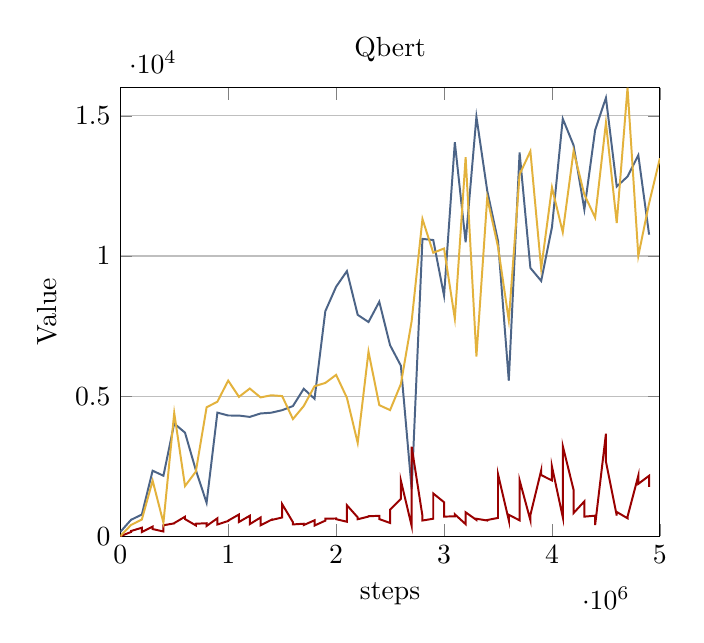
\begin{tikzpicture}

\begin{axis}[%
title=Qbert,
% %width=4.634in,
%width=10in,
%height=5in,
%at={(2.596in,2.358in)},
% scale only axis,
xmin=0,
xmax=5000000,
xlabel style={font=\color{white!15!black}},
xlabel={steps},
xlabel near ticks,
ymin=0,
ymax=16000,
ylabel style={font=\color{white!15!black}},
ylabel={Value},
ylabel near ticks,
ymajorgrids,
% %scale=0.5,
%scale=0.4,
axis background/.style={fill=white},
%legend style={legend cell align=left, align=left, draw=white!15!black}
]
\addplot [color=blue, line width = 0.25mm]
                table[row sep=crcr]{
                  0 150.0\\ 
100000 585.0\\ 
200000 772.5\\ 
300000 2337.5\\ 
400000 2157.5\\ 
500000 4022.5\\ 
600000 3695.0\\ 
700000 2362.5\\ 
800000 1192.5\\ 
900000 4410.0\\ 
1000000 4307.5\\ 
1100000 4305.0\\ 
1200000 4257.5\\ 
1300000 4380.0\\ 
1400000 4407.5\\ 
1500000 4497.5\\ 
1600000 4645.0\\ 
1700000 5260.0\\ 
1800000 4905.0\\ 
1900000 8030.0\\ 
2000000 8902.5\\ 
2100000 9460.0\\ 
2200000 7900.0\\ 
2300000 7642.5\\ 
2400000 8367.5\\ 
2500000 6815.0\\ 
2600000 6085.0\\ 
2700000 1677.5\\ 
2800000 10610.0\\ 
2900000 10570.0\\ 
3000000 8585.0\\ 
3100000 14057.5\\ 
3200000 10490.0\\ 
3300000 14970.0\\ 
3400000 12332.5\\ 
3500000 10537.5\\ 
3600000 5550.0\\ 
3700000 13692.5\\ 
3800000 9572.5\\ 
3900000 9110.0\\ 
4000000 11030.0\\ 
4100000 14897.5\\ 
4200000 13955.0\\ 
4300000 11660.0\\ 
4400000 14495.0\\ 
4500000 15645.0\\ 
4600000 12480.0\\ 
4700000 12835.0\\ 
4800000 13597.5\\ 
4900000 10762.5\\ 
};
\addplot [color=red, line width = 0.25mm]
                table[row sep=crcr]{
                  0 0.0\\ 
0 0.0\\ 
100000 150.0\\ 
100000 185.0\\ 
200000 302.5\\ 
200000 150.0\\ 
300000 342.5\\ 
300000 255.0\\ 
400000 167.5\\ 
400000 390.0\\ 
500000 457.5\\ 
500000 467.5\\ 
600000 695.0\\ 
600000 610.0\\ 
700000 385.0\\ 
700000 445.0\\ 
800000 462.5\\ 
800000 365.0\\ 
900000 640.0\\ 
900000 417.5\\ 
1000000 542.5\\ 
1000000 555.0\\ 
1100000 775.0\\ 
1100000 507.5\\ 
1200000 730.0\\ 
1200000 430.0\\ 
1300000 667.5\\ 
1300000 387.5\\ 
1400000 585.0\\ 
1400000 577.5\\ 
1500000 667.5\\ 
1500000 1145.0\\ 
1600000 500.0\\ 
1600000 420.0\\ 
1700000 445.0\\ 
1700000 397.5\\ 
1800000 567.5\\ 
1800000 380.0\\ 
1900000 555.0\\ 
1900000 625.0\\ 
2000000 632.5\\ 
2000000 607.5\\ 
2100000 515.0\\ 
2100000 1105.0\\ 
2200000 672.5\\ 
2200000 605.0\\ 
2300000 700.0\\ 
2300000 712.5\\ 
2400000 727.5\\ 
2400000 610.0\\ 
2500000 472.5\\ 
2500000 947.5\\ 
2600000 1330.0\\ 
2600000 1985.0\\ 
2700000 365.0\\ 
2700000 3195.0\\ 
2800000 720.0\\ 
2800000 560.0\\ 
2900000 622.5\\ 
2900000 1525.0\\ 
3000000 1212.5\\ 
3000000 700.0\\ 
3100000 707.5\\ 
3100000 780.0\\ 
3200000 430.0\\ 
3200000 852.5\\ 
3300000 580.0\\ 
3300000 622.5\\ 
3400000 560.0\\ 
3400000 577.5\\ 
3500000 652.5\\ 
3500000 2215.0\\ 
3600000 567.5\\ 
3600000 765.0\\ 
3700000 565.0\\ 
3700000 1995.0\\ 
3800000 570.0\\ 
3800000 757.5\\ 
3900000 2345.0\\ 
3900000 2182.5\\ 
4000000 1987.5\\ 
4000000 2482.5\\ 
4100000 682.5\\ 
4100000 3220.0\\ 
4200000 1657.5\\ 
4200000 825.0\\ 
4300000 1242.5\\ 
4300000 697.5\\ 
4400000 732.5\\ 
4400000 397.5\\ 
4500000 3660.0\\ 
4500000 2662.5\\ 
4600000 735.0\\ 
4600000 865.0\\ 
4700000 640.0\\ 
4700000 695.0\\ 
4800000 2160.0\\ 
4800000 1867.5\\ 
4900000 2157.5\\ 
4900000 1762.5\\ 
};
\addplot [color=yellow, line width = 0.25mm]
                table[row sep=crcr]{
                  0 0.0\\ 
0 0.0\\ 
0 0.0\\ 
0 0.0\\ 
100000 400.0\\ 
200000 595.0\\ 
300000 1982.5\\ 
400000 480.0\\ 
500000 4397.5\\ 
600000 1790.0\\ 
700000 2302.5\\ 
800000 4600.0\\ 
900000 4800.0\\ 
1000000 5552.5\\ 
1100000 4972.5\\ 
1200000 5270.0\\ 
1300000 4952.5\\ 
1400000 5030.0\\ 
1500000 5000.0\\ 
1600000 4180.0\\ 
1700000 4645.0\\ 
1800000 5352.5\\ 
1900000 5470.0\\ 
2000000 5757.5\\ 
2100000 4940.0\\ 
2200000 3327.5\\ 
2300000 6585.0\\ 
2400000 4677.5\\ 
2500000 4500.0\\ 
2600000 5430.0\\ 
2700000 7677.5\\ 
2800000 11320.0\\ 
2900000 10115.0\\ 
3000000 10267.5\\ 
3100000 7765.0\\ 
3200000 13525.0\\ 
3300000 6415.0\\ 
3400000 12077.5\\ 
3500000 10327.5\\ 
3600000 7700.0\\ 
3700000 12912.5\\ 
3800000 13737.5\\ 
3900000 9552.5\\ 
4000000 12445.0\\ 
4100000 10847.5\\ 
4200000 13737.5\\ 
4300000 12195.0\\ 
4400000 11370.0\\ 
4500000 14755.0\\ 
4600000 11175.0\\ 
4700000 16002.5\\ 
4800000 10005.0\\ 
4900000 11885.0\\ 
5000000 13490.0\\ 
};
\end{axis}
\end{tikzpicture}}}
    \subfloat[]{  \resizebox{0.4\textwidth}{!}{
\definecolor{blue}{RGB}{76,100,135}
\definecolor{red}{RGB}{153,0,0}
\definecolor{yellow}{RGB}{227,178,60}
\definecolor{mycolor1}{rgb}{0.00000,0.44700,0.74100}%
\definecolor{mycolor2}{rgb}{0.85000,0.32500,0.09800}%
\definecolor{mycolor3}{rgb}{0.92900,0.69400,0.12500}%
%
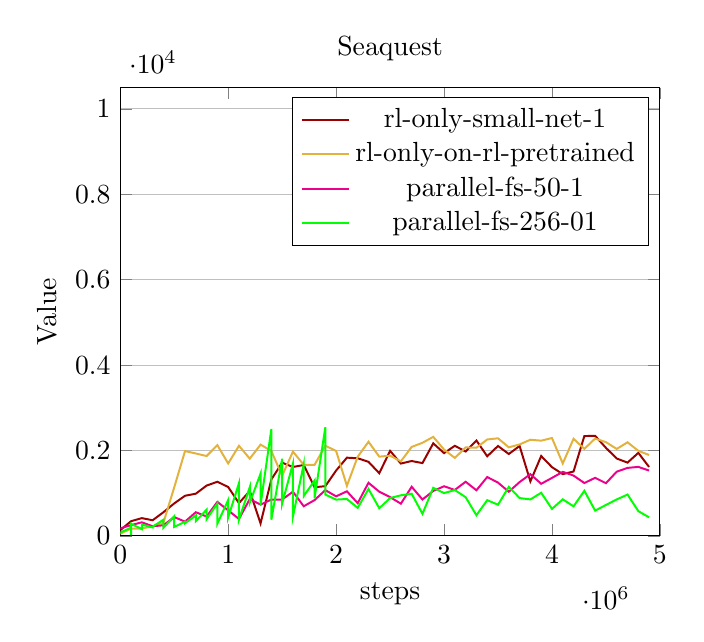
\begin{tikzpicture}

\begin{axis}[%
title=Seaquest,
% %width=4.634in,
%width=10in,
%height=5in,
%at={(2.596in,2.358in)},
% scale only axis,
xmin=0,
xmax=5000000,
xlabel style={font=\color{white!15!black}},
xlabel={steps},
xlabel near ticks,
ymin=0,
ymax=10500,
ylabel style={font=\color{white!15!black}},
ylabel={Value},
ylabel near ticks,
ymajorgrids,
% %scale=0.5,
%scale=0.4,
axis background/.style={fill=white},
%legend style={legend cell align=left, align=left, draw=white!15!black}
]
\addplot [color=red, line width = 0.25mm]
                table[row sep=crcr]{
                  0 134.0\\ 
100000 344.0\\ 
200000 416.0\\ 
300000 366.0\\ 
400000 554.0\\ 
500000 760.0\\ 
600000 940.0\\ 
700000 988.0\\ 
800000 1178.0\\ 
900000 1268.0\\ 
1000000 1144.0\\ 
1100000 768.0\\ 
1200000 1052.0\\ 
1300000 292.0\\ 
1400000 1322.0\\ 
1500000 1714.0\\ 
1600000 1614.0\\ 
1700000 1660.0\\ 
1800000 1140.0\\ 
1900000 1164.0\\ 
2000000 1530.0\\ 
2100000 1832.0\\ 
2200000 1818.0\\ 
2300000 1734.0\\ 
2400000 1468.0\\ 
2500000 1992.0\\ 
2600000 1694.0\\ 
2700000 1754.0\\ 
2800000 1704.0\\ 
2900000 2168.0\\ 
3000000 1938.0\\ 
3100000 2110.0\\ 
3200000 1976.0\\ 
3300000 2234.0\\ 
3400000 1864.0\\ 
3500000 2106.0\\ 
3600000 1918.0\\ 
3700000 2106.0\\ 
3800000 1276.0\\ 
3900000 1870.0\\ 
4000000 1610.0\\ 
4100000 1446.0\\ 
4200000 1508.0\\ 
4300000 2338.0\\ 
4400000 2344.0\\ 
4500000 2062.0\\ 
4600000 1812.0\\ 
4700000 1716.0\\ 
4800000 1944.0\\ 
4900000 1614.0\\ 
};
\addlegendentry{rl-only-small-net-1}
\addplot [color=yellow, line width = 0.25mm]
                table[row sep=crcr]{
                  0 48.0\\ 
100000 172.0\\ 
200000 172.0\\ 
300000 224.0\\ 
400000 308.0\\ 
500000 1136.0\\ 
600000 1986.0\\ 
700000 1930.0\\ 
800000 1870.0\\ 
900000 2124.0\\ 
1000000 1696.0\\ 
1100000 2110.0\\ 
1200000 1808.0\\ 
1300000 2138.0\\ 
1400000 1988.0\\ 
1500000 1408.0\\ 
1600000 1974.0\\ 
1700000 1664.0\\ 
1800000 1662.0\\ 
1900000 2112.0\\ 
2000000 1990.0\\ 
2100000 1172.0\\ 
2200000 1854.0\\ 
2300000 2204.0\\ 
2400000 1856.0\\ 
2500000 1878.0\\ 
2600000 1746.0\\ 
2700000 2084.0\\ 
2800000 2180.0\\ 
2900000 2320.0\\ 
3000000 2022.0\\ 
3100000 1826.0\\ 
3200000 2072.0\\ 
3300000 2064.0\\ 
3400000 2258.0\\ 
3500000 2286.0\\ 
3600000 2074.0\\ 
3700000 2142.0\\ 
3800000 2252.0\\ 
3900000 2230.0\\ 
4000000 2292.0\\ 
4100000 1696.0\\ 
4200000 2274.0\\ 
4300000 2038.0\\ 
4400000 2280.0\\ 
4500000 2196.0\\ 
4600000 2036.0\\ 
4700000 2192.0\\ 
4800000 1992.0\\ 
4900000 1894.0\\ 
};
\addlegendentry{rl-only-on-rl-pretrained}
\addplot [color=magenta, line width = 0.25mm]
                table[row sep=crcr]{
                  0 176.0\\ 
0 176.0\\ 
100000 252.0\\ 
200000 318.0\\ 
300000 226.0\\ 
400000 248.0\\ 
500000 440.0\\ 
600000 334.0\\ 
700000 554.0\\ 
800000 454.0\\ 
900000 796.0\\ 
1000000 598.0\\ 
1100000 396.0\\ 
1200000 862.0\\ 
1300000 732.0\\ 
1400000 850.0\\ 
1500000 852.0\\ 
1600000 1034.0\\ 
1700000 694.0\\ 
1800000 838.0\\ 
1900000 1072.0\\ 
2000000 926.0\\ 
2100000 1044.0\\ 
2200000 766.0\\ 
2300000 1244.0\\ 
2400000 1034.0\\ 
2500000 908.0\\ 
2600000 754.0\\ 
2700000 1150.0\\ 
2800000 852.0\\ 
2900000 1052.0\\ 
3000000 1162.0\\ 
3100000 1076.0\\ 
3200000 1268.0\\ 
3300000 1068.0\\ 
3400000 1378.0\\ 
3500000 1248.0\\ 
3600000 1034.0\\ 
3700000 1260.0\\ 
3800000 1446.0\\ 
3900000 1220.0\\ 
4000000 1358.0\\ 
4100000 1500.0\\ 
4200000 1412.0\\ 
4300000 1238.0\\ 
4400000 1360.0\\ 
4500000 1234.0\\ 
4600000 1504.0\\ 
4700000 1592.0\\ 
4800000 1616.0\\ 
4900000 1530.0\\ 
};
\addlegendentry{parallel-fs-50-1}
\addplot [color=green, line width = 0.25mm]
                table[row sep=crcr]{
                  0 80.0\\ 
0 80.0\\ 
0 80.0\\ 
100000 192.0\\ 
100000 20.0\\ 
100000 284.0\\ 
200000 158.0\\ 
200000 264.0\\ 
300000 198.0\\ 
300000 216.0\\ 
400000 378.0\\ 
400000 192.0\\ 
500000 460.0\\ 
500000 210.0\\ 
600000 330.0\\ 
600000 296.0\\ 
700000 478.0\\ 
700000 344.0\\ 
800000 614.0\\ 
800000 390.0\\ 
900000 758.0\\ 
900000 288.0\\ 
1000000 840.0\\ 
1000000 432.0\\ 
1100000 1236.0\\ 
1100000 384.0\\ 
1200000 1142.0\\ 
1200000 776.0\\ 
1300000 1458.0\\ 
1300000 730.0\\ 
1400000 2504.0\\ 
1400000 380.0\\ 
1500000 1806.0\\ 
1500000 756.0\\ 
1600000 1695.0\\ 
1600000 454.0\\ 
1700000 1678.0\\ 
1700000 932.0\\ 
1800000 1296.0\\ 
1800000 878.0\\ 
1900000 2544.0\\ 
1900000 968.0\\ 
2000000 850.0\\ 
2100000 864.0\\ 
2200000 656.0\\ 
2300000 1098.0\\ 
2400000 648.0\\ 
2500000 886.0\\ 
2600000 950.0\\ 
2700000 988.0\\ 
2800000 516.0\\ 
2900000 1126.0\\ 
3000000 1002.0\\ 
3100000 1074.0\\ 
3200000 906.0\\ 
3300000 484.0\\ 
3400000 836.0\\ 
3500000 730.0\\ 
3600000 1148.0\\ 
3700000 886.0\\ 
3800000 854.0\\ 
3900000 1010.0\\ 
4000000 632.0\\ 
4100000 856.0\\ 
4200000 692.0\\ 
4300000 1056.0\\ 
4400000 592.0\\ 
4500000 724.0\\ 
4600000 854.0\\ 
4700000 968.0\\ 
4800000 580.0\\ 
4900000 434.0\\ 
};
\addlegendentry{parallel-fs-256-01}
\end{axis}
\end{tikzpicture}}}\\
  \vspace{-1cm}
    \subfloat[]{  \resizebox{0.4\textwidth}{!}{
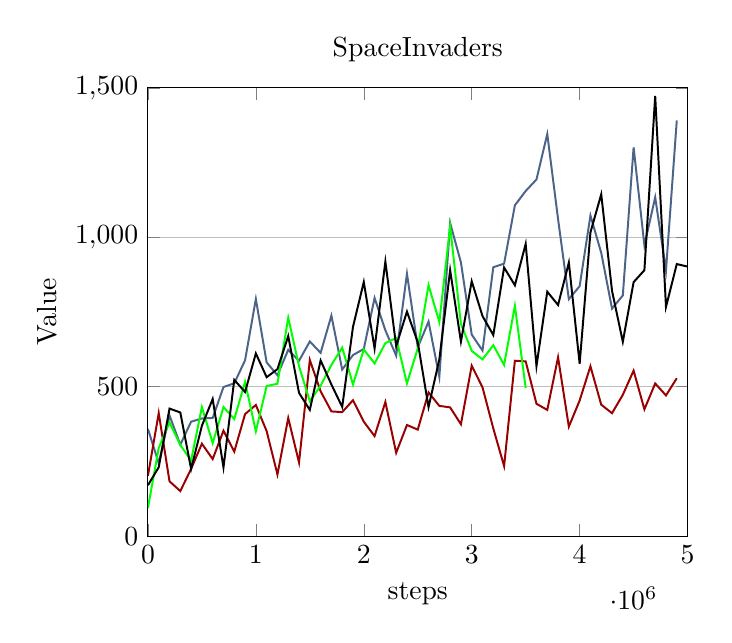
\begin{tikzpicture}

\begin{axis}[%
title=SpaceInvaders,
%width=10in,
%height=5in,
%at={(2.596in,2.358in)},
% scale only axis,
xmin=0,
xmax=5000000,
xlabel style={font=\color{white!15!black}},
xlabel={steps},
xlabel near ticks,
ymin=0,
ymax=1500,
ylabel style={font=\color{white!15!black}},
ylabel={Value},
ylabel near ticks,
ymajorgrids,
% %scale=0.5,
%scale=0.4,
axis background/.style={fill=white},
%legend style={legend cell align=left, align=left, draw=white!15!black}
]
\addplot [color=blue, line width = 0.25mm]
                table[row sep=crcr]{
                  0 359.0\\ 
100000 244.0\\ 
200000 404.0\\ 
300000 306.0\\ 
400000 383.0\\ 
500000 394.0\\ 
600000 395.5\\ 
700000 499.0\\ 
800000 511.5\\ 
900000 588.5\\ 
1000000 793.5\\ 
1100000 581.5\\ 
1200000 538.5\\ 
1300000 623.5\\ 
1400000 587.0\\ 
1500000 651.5\\ 
1600000 613.5\\ 
1700000 738.0\\ 
1800000 557.5\\ 
1900000 606.0\\ 
2000000 626.5\\ 
2100000 797.0\\ 
2200000 689.0\\ 
2300000 604.0\\ 
2400000 878.0\\ 
2500000 632.0\\ 
2600000 718.0\\ 
2700000 533.0\\ 
2800000 1048.0\\ 
2900000 916.0\\ 
3000000 674.5\\ 
3100000 621.0\\ 
3200000 900.0\\ 
3300000 912.0\\ 
3400000 1107.0\\ 
3500000 1155.0\\ 
3600000 1193.5\\ 
3700000 1345.5\\ 
3800000 1061.0\\ 
3900000 793.0\\ 
4000000 836.5\\ 
4100000 1073.0\\ 
4200000 948.0\\ 
4300000 761.5\\ 
4400000 805.5\\ 
4500000 1301.0\\ 
4600000 973.0\\ 
4700000 1134.0\\ 
4800000 889.5\\ 
4900000 1391.0\\ 
};
\addplot [color=red, line width = 0.25mm]
                table[row sep=crcr]{
                  0 202.0\\ 
100000 412.0\\ 
200000 183.5\\ 
300000 151.0\\ 
400000 225.0\\ 
500000 309.5\\ 
600000 258.0\\ 
700000 353.0\\ 
800000 283.0\\ 
900000 408.5\\ 
1000000 439.0\\ 
1100000 351.5\\ 
1200000 206.5\\ 
1300000 395.5\\ 
1400000 246.5\\ 
1500000 589.5\\ 
1600000 485.0\\ 
1700000 417.5\\ 
1800000 415.0\\ 
1900000 455.0\\ 
2000000 383.0\\ 
2100000 335.0\\ 
2200000 449.0\\ 
2300000 279.0\\ 
2400000 372.0\\ 
2500000 356.5\\ 
2600000 481.0\\ 
2700000 436.0\\ 
2800000 431.0\\ 
2900000 374.5\\ 
3000000 570.5\\ 
3100000 498.0\\ 
3200000 360.5\\ 
3300000 234.5\\ 
3400000 587.0\\ 
3500000 585.0\\ 
3600000 443.0\\ 
3700000 422.5\\ 
3800000 598.5\\ 
3900000 366.5\\ 
4000000 454.0\\ 
4100000 568.5\\ 
4200000 440.0\\ 
4300000 411.5\\ 
4400000 473.0\\ 
4500000 554.0\\ 
4600000 424.5\\ 
4700000 511.0\\ 
4800000 471.0\\ 
4900000 528.5\\ 
};
\addplot [color=green, line width = 0.25mm]
                table[row sep=crcr]{
                  0 94.5\\ 
100000 295.0\\ 
200000 380.5\\ 
300000 305.0\\ 
400000 253.0\\ 
500000 432.0\\ 
600000 311.5\\ 
700000 432.0\\ 
800000 392.0\\ 
900000 516.0\\ 
1000000 351.0\\ 
1100000 502.5\\ 
1200000 510.0\\ 
1300000 731.0\\ 
1400000 569.0\\ 
1500000 451.5\\ 
1600000 503.5\\ 
1700000 573.0\\ 
1800000 631.0\\ 
1900000 507.5\\ 
2000000 624.5\\ 
2100000 578.0\\ 
2200000 646.0\\ 
2300000 663.0\\ 
2400000 511.0\\ 
2500000 628.0\\ 
2600000 840.0\\ 
2700000 716.5\\ 
2800000 1037.0\\ 
2900000 710.5\\ 
3000000 620.0\\ 
3100000 591.5\\ 
3200000 639.0\\ 
3300000 573.0\\ 
3400000 771.0\\ 
3500000 496.0\\ 
};
\addplot [color=black, line width = 0.25mm]
                table[row sep=crcr]{
                  0 170.5\\ 
100000 230.5\\ 
200000 427.0\\ 
300000 414.0\\ 
400000 225.0\\ 
500000 369.5\\ 
600000 459.0\\ 
700000 230.0\\ 
800000 523.0\\ 
900000 482.5\\ 
1000000 611.5\\ 
1100000 532.0\\ 
1200000 559.0\\ 
1300000 669.5\\ 
1400000 479.5\\ 
1500000 422.5\\ 
1600000 588.0\\ 
1700000 507.5\\ 
1800000 432.5\\ 
1900000 700.5\\ 
2000000 850.5\\ 
2100000 628.0\\ 
2200000 919.0\\ 
2300000 636.0\\ 
2400000 751.5\\ 
2500000 649.0\\ 
2600000 432.0\\ 
2700000 591.5\\ 
2800000 890.0\\ 
2900000 651.0\\ 
3000000 853.0\\ 
3100000 736.5\\ 
3200000 673.0\\ 
3300000 899.0\\ 
3400000 839.5\\ 
3500000 978.0\\ 
3600000 569.0\\ 
3700000 818.0\\ 
3800000 773.5\\ 
3900000 915.5\\ 
4000000 577.0\\ 
4100000 1016.5\\ 
4200000 1144.0\\ 
4300000 821.0\\ 
4400000 650.5\\ 
4500000 850.0\\ 
4600000 890.0\\ 
4700000 1473.0\\ 
4800000 767.0\\ 
4900000 910.5\\ 
5000000 902.0\\ 
};
\end{axis}
\end{tikzpicture}}}
  \\

  \ref{named}
  \caption{Comparison of using and L2 latent space regularization and data augmentation in parallel training.
  L2 regularization helps overall because it helps fix the latent representations in place, thereby stabilizing
the overall training process. Data augmentation on the other hand clearly hurt across the board.}
  \label{fig:reg-vs-no-reg}
\end{figure}

As can be seen in the figure \ref{fig:reg-vs-no-reg}, regularization can both benefit and hurt learning.
L2 regularization forces the latent space to be distributed more closely to the origin. While somewhat arbitrary,
we checked that it substantially helps in maintaining the same latent vectors for the same inputs
across updates. This was measured by observing the reconstruction quality over encoders and decoders
saved at different epochs.

Data augmentation seems to only add noise and therefore hurt learning by destabilizing it.
This might be due to our particular implementation, but it is more likely due to the fact that 
the encoder produces different outputs for the same, but differently augmented input.


\section{Effectiveness of forward prediction}
\label{sec-effectiveness-of-forward}
Finally, we compare the effectiveness of forward prediction, or
the importance of dynamics for state representations.
The results can be observed in \ref{fig:forward-vs-compression}.

\begin{figure}[!t]
  \captionsetup[subfloat]{position=top,labelformat=empty}
  \vspace{-1.5cm}
  \centering

    \subfloat[]{  \resizebox{0.4\textwidth}{!}{
%\definecolor{blue}{RGB}{76,100,135}
%\definecolor{red}{RGB}{153,0,0}
%\definecolor{yellow}{RGB}{227,178,60}
%\definecolor{mycolor1}{rgb}{0.00000,0.44700,0.74100}%
%\definecolor{mycolor2}{rgb}{0.85000,0.32500,0.09800}%
%\definecolor{mycolor3}{rgb}{0.92900,0.69400,0.12500}%
%
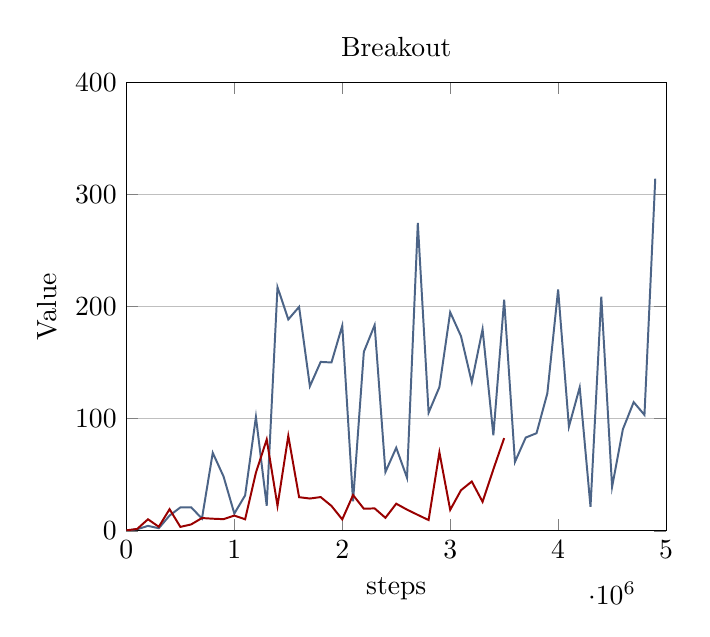
\begin{tikzpicture}

\begin{axis}[%
legend entries={rl-only-small-net,L2-reg,parallel-fs-50-no-aug}, 
legend columns=2,
title=Breakout,
legend to name=named,
legend style={legend cell align=left},
%%width=10in,
%%height=5in,
%%at={(2.596in,2.358in)},
% scale only axis,
xmin=0,
xmax=5000000,
xlabel style={font=\color{white!15!black}},
xlabel={steps},
xlabel near ticks,
ymin=0,
ymax=400,
ylabel style={font=\color{white!15!black}},
ylabel={Value},
ylabel near ticks,
ymajorgrids,
% %scale=0.5,
%%scale=0.4,
axis background/.style={fill=white},
%legend columns=2,
%legend=south outside
]
\addplot [color=blue, line width = 0.25mm]
                table[row sep=crcr]{
                  0 0.20000000298023224\\ 
100000 1.399999976158142\\ 
200000 4.400000095367432\\ 
300000 2.299999952316284\\ 
400000 13.600000381469727\\ 
500000 20.899999618530273\\ 
600000 21.0\\ 
700000 10.899999618530273\\ 
800000 69.5999984741211\\ 
900000 48.5\\ 
1000000 15.399999618530273\\ 
1100000 31.600000381469727\\ 
1200000 101.5999984741211\\ 
1300000 22.399999618530273\\ 
1400000 217.39999389648438\\ 
1500000 188.60000610351562\\ 
1600000 199.8000030517578\\ 
1700000 129.0\\ 
1800000 150.6999969482422\\ 
1900000 150.1999969482422\\ 
2000000 183.0\\ 
2100000 26.399999618530273\\ 
2200000 159.6999969482422\\ 
2300000 183.5\\ 
2400000 52.5\\ 
2500000 74.0999984741211\\ 
2600000 47.29999923706055\\ 
2700000 274.6000061035156\\ 
2800000 105.4000015258789\\ 
2900000 128.1999969482422\\ 
3000000 195.0\\ 
3100000 173.6999969482422\\ 
3200000 132.60000610351562\\ 
3300000 179.89999389648438\\ 
3400000 85.19999694824219\\ 
3500000 206.1999969482422\\ 
3600000 61.5\\ 
3700000 83.19999694824219\\ 
3800000 87.0999984741211\\ 
3900000 122.5999984741211\\ 
4000000 215.3000030517578\\ 
4100000 92.9000015258789\\ 
4200000 128.0\\ 
4300000 21.399999618530273\\ 
4400000 208.89999389648438\\ 
4500000 39.20000076293945\\ 
4600000 90.5999984741211\\ 
4700000 114.80000305175781\\ 
4800000 103.4000015258789\\ 
4900000 314.20001220703125\\ 
};
\addplot [color=red, line width = 0.25mm]
                table[row sep=crcr]{
                  0 0.4000000059604645\\ 
100000 1.7000000476837158\\ 
200000 10.300000190734863\\ 
300000 3.5999999046325684\\ 
400000 19.299999237060547\\ 
500000 3.5\\ 
600000 5.699999809265137\\ 
700000 11.399999618530273\\ 
800000 10.800000190734863\\ 
900000 10.399999618530273\\ 
1000000 13.600000381469727\\ 
1100000 10.300000190734863\\ 
1200000 51.900001525878906\\ 
1300000 81.5\\ 
1400000 22.299999237060547\\ 
1500000 84.69999694824219\\ 
1600000 30.0\\ 
1700000 28.799999237060547\\ 
1800000 30.100000381469727\\ 
1900000 22.200000762939453\\ 
2000000 10.199999809265137\\ 
2100000 31.899999618530273\\ 
2200000 19.700000762939453\\ 
2300000 20.0\\ 
2400000 11.600000381469727\\ 
2500000 24.200000762939453\\ 
2600000 18.899999618530273\\ 
2700000 14.199999809265137\\ 
2800000 9.600000381469727\\ 
2900000 70.0\\ 
3000000 18.700000762939453\\ 
3100000 36.20000076293945\\ 
3200000 44.0\\ 
3300000 25.899999618530273\\ 
3400000 54.900001525878906\\ 
3500000 82.69999694824219\\ 
};
\addplot [color=yellow, line width = 0.25mm]
                table[row sep=crcr]{
                  0 0.800000011920929\\ 
};
\end{axis}
\end{tikzpicture}}}
    \subfloat[]{  \resizebox{0.4\textwidth}{!}{
%\definecolor{blue}{RGB}{76,100,135}
%\definecolor{red}{RGB}{153,0,0}
%\definecolor{yellow}{RGB}{227,178,60}
%\definecolor{mycolor1}{rgb}{0.00000,0.44700,0.74100}%
%\definecolor{mycolor2}{rgb}{0.85000,0.32500,0.09800}%
%\definecolor{mycolor3}{rgb}{0.92900,0.69400,0.12500}%
%
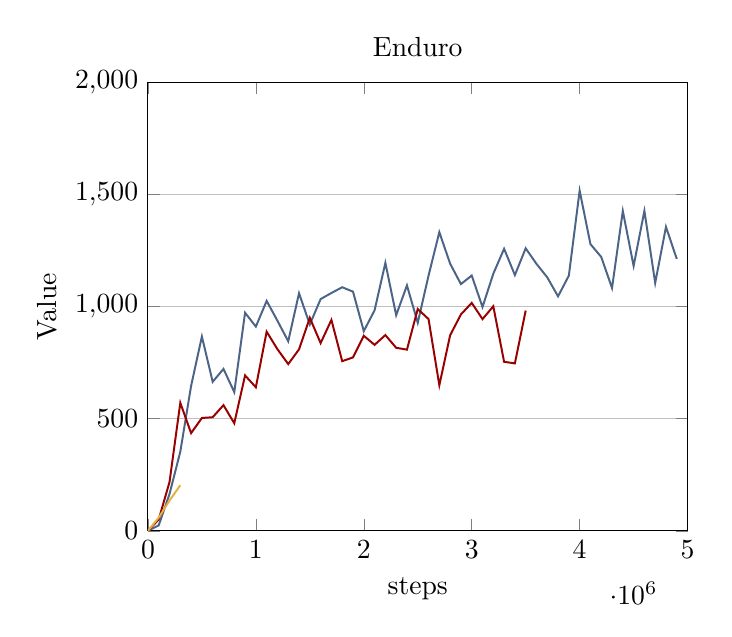
\begin{tikzpicture}

\begin{axis}[%
title=Enduro,
% %width=4.634in,
%%width=10in,
%%height=5in,
%at={(2.596in,2.358in)},
% scale only axis,
xmin=0,
xmax=5000000,
xlabel style={font=\color{white!15!black}},
xlabel={steps},
xlabel near ticks,
ymin=0,
ymax=2000,
ylabel style={font=\color{white!15!black}},
ylabel={Value},
ylabel near ticks,
ymajorgrids,
% %scale=0.5,
%scale=0.4,
axis background/.style={fill=white},
%legend style={legend cell align=left, align=left, draw=white!15!black}
]
\addplot [color=blue, line width = 0.25mm]
                table[row sep=crcr]{
                  0 0.0\\ 
100000 24.299999237060547\\ 
200000 164.3000030517578\\ 
300000 353.0\\ 
400000 646.4000244140625\\ 
500000 866.7000122070312\\ 
600000 664.7000122070312\\ 
700000 722.2000122070312\\ 
800000 618.9000244140625\\ 
900000 972.7999877929688\\ 
1000000 910.9000244140625\\ 
1100000 1025.699951171875\\ 
1200000 937.0\\ 
1300000 845.5999755859375\\ 
1400000 1059.9000244140625\\ 
1500000 920.2999877929688\\ 
1600000 1033.800048828125\\ 
1700000 1061.0\\ 
1800000 1086.5999755859375\\ 
1900000 1066.9000244140625\\ 
2000000 890.9000244140625\\ 
2100000 983.5\\ 
2200000 1195.300048828125\\ 
2300000 962.0\\ 
2400000 1094.800048828125\\ 
2500000 928.0\\ 
2600000 1138.5999755859375\\ 
2700000 1332.300048828125\\ 
2800000 1191.800048828125\\ 
2900000 1100.5999755859375\\ 
3000000 1138.800048828125\\ 
3100000 998.2999877929688\\ 
3200000 1146.800048828125\\ 
3300000 1258.0999755859375\\ 
3400000 1141.0\\ 
3500000 1260.300048828125\\ 
3600000 1190.800048828125\\ 
3700000 1130.5999755859375\\ 
3800000 1046.0999755859375\\ 
3900000 1138.4000244140625\\ 
4000000 1517.5\\ 
4100000 1278.9000244140625\\ 
4200000 1221.699951171875\\ 
4300000 1083.199951171875\\ 
4400000 1426.9000244140625\\ 
4500000 1181.5999755859375\\ 
4600000 1427.199951171875\\ 
4700000 1105.800048828125\\ 
4800000 1355.800048828125\\ 
4900000 1212.9000244140625\\ 
};
\addplot [color=red, line width = 0.25mm]
                table[row sep=crcr]{
                  0 0.0\\ 
100000 50.5\\ 
200000 217.60000610351562\\ 
300000 570.9000244140625\\ 
400000 435.6000061035156\\ 
500000 503.3999938964844\\ 
600000 506.79998779296875\\ 
700000 560.5\\ 
800000 479.79998779296875\\ 
900000 693.2000122070312\\ 
1000000 640.4000244140625\\ 
1100000 888.4000244140625\\ 
1200000 810.0999755859375\\ 
1300000 743.7999877929688\\ 
1400000 809.5\\ 
1500000 950.2000122070312\\ 
1600000 837.4000244140625\\ 
1700000 940.7999877929688\\ 
1800000 756.7999877929688\\ 
1900000 773.5\\ 
2000000 870.0999755859375\\ 
2100000 829.5999755859375\\ 
2200000 873.2000122070312\\ 
2300000 816.5\\ 
2400000 808.2000122070312\\ 
2500000 989.5999755859375\\ 
2600000 944.5\\ 
2700000 649.4000244140625\\ 
2800000 872.4000244140625\\ 
2900000 965.2000122070312\\ 
3000000 1016.7000122070312\\ 
3100000 944.4000244140625\\ 
3200000 1001.7000122070312\\ 
3300000 754.0\\ 
3400000 746.7999877929688\\ 
3500000 982.2999877929688\\ 
};
\addplot [color=yellow, line width = 0.25mm]
                table[row sep=crcr]{
                  0 0.0\\ 
100000 58.79999923706055\\ 
200000 135.10000610351562\\ 
300000 203.1999969482422\\ 
};
\end{axis}
\end{tikzpicture}}}\\
  \vspace{-1cm}
    \subfloat[]{  \resizebox{0.4\textwidth}{!}{
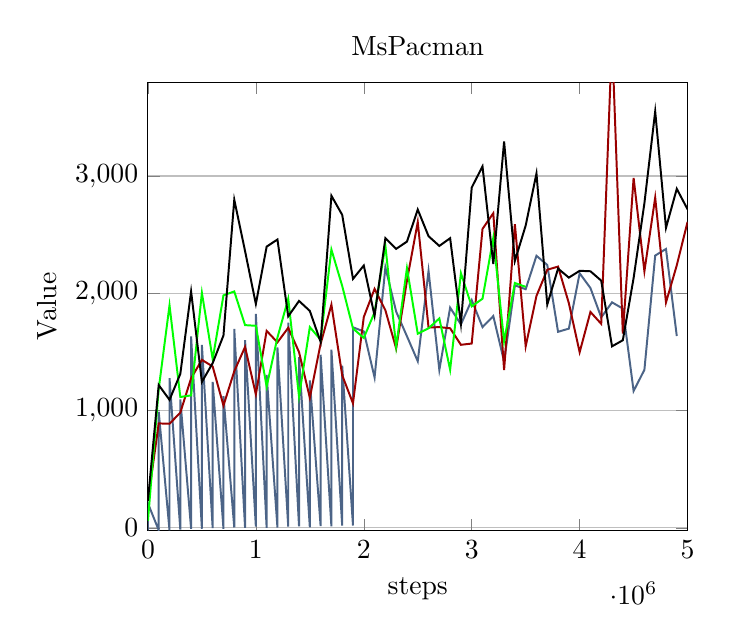
\begin{tikzpicture}

\begin{axis}[%
title=MsPacman,
% %width=4.634in,
%width=10in,
%height=5in,
%at={(2.596in,2.358in)},
% scale only axis,
xmin=0,
xmax=5000000,
xlabel style={font=\color{white!15!black}},
xlabel={steps},
xlabel near ticks,
ymin=-22,
ymax=3800,
ylabel style={font=\color{white!15!black}},
ylabel={Value},
ylabel near ticks,
ymajorgrids,
% %scale=0.5,
%scale=0.4,
axis background/.style={fill=white},
%legend style={legend cell align=left, align=left, draw=white!15!black}
]
\addplot [color=blue, line width = 0.25mm]
                table[row sep=crcr]{
                  0 -21.0\\ 
0 210.0\\ 
100000 -19.799999237060547\\ 
100000 990.0\\ 
200000 -20.700000762939453\\ 
200000 1277.0\\ 
300000 -15.0\\ 
300000 1096.0\\ 
400000 -7.0\\ 
400000 1632.0\\ 
500000 -6.900000095367432\\ 
500000 1561.0\\ 
600000 -1.899999976158142\\ 
600000 1245.0\\ 
700000 -7.599999904632568\\ 
700000 1123.0\\ 
800000 4.0\\ 
800000 1696.0\\ 
900000 1.5\\ 
900000 1600.0\\ 
1000000 11.300000190734863\\ 
1000000 1824.0\\ 
1100000 1.2000000476837158\\ 
1100000 1304.0\\ 
1200000 3.700000047683716\\ 
1200000 1538.0\\ 
1300000 11.5\\ 
1300000 1750.0\\ 
1400000 13.600000381469727\\ 
1400000 1456.0\\ 
1500000 5.699999809265137\\ 
1500000 1258.0\\ 
1600000 15.600000381469727\\ 
1600000 1476.0\\ 
1700000 13.5\\ 
1700000 1519.0\\ 
1800000 19.299999237060547\\ 
1800000 1383.0\\ 
1900000 20.799999237060547\\ 
1900000 1710.0\\ 
2000000 1675.0\\ 
2100000 1282.0\\ 
2200000 2222.0\\ 
2300000 1844.0\\ 
2400000 1634.0\\ 
2500000 1421.0\\ 
2600000 2191.0\\ 
2700000 1347.0\\ 
2800000 1878.0\\ 
2900000 1735.0\\ 
3000000 1942.0\\ 
3100000 1712.0\\ 
3200000 1806.0\\ 
3300000 1419.0\\ 
3400000 2068.0\\ 
3500000 2035.0\\ 
3600000 2320.0\\ 
3700000 2242.0\\ 
3800000 1672.0\\ 
3900000 1699.0\\ 
4000000 2171.0\\ 
4100000 2045.0\\ 
4200000 1795.0\\ 
4300000 1923.0\\ 
4400000 1870.0\\ 
4500000 1167.0\\ 
4600000 1348.0\\ 
4700000 2322.0\\ 
4800000 2378.0\\ 
4900000 1636.0\\ 
};
\addplot [color=red, line width = 0.25mm]
                table[row sep=crcr]{
                  0 230.0\\ 
100000 891.0\\ 
200000 888.0\\ 
300000 983.0\\ 
400000 1276.0\\ 
500000 1433.0\\ 
600000 1376.0\\ 
700000 1043.0\\ 
800000 1336.0\\ 
900000 1543.0\\ 
1000000 1139.0\\ 
1100000 1680.0\\ 
1200000 1582.0\\ 
1300000 1706.0\\ 
1400000 1499.0\\ 
1500000 1110.0\\ 
1600000 1569.0\\ 
1700000 1903.0\\ 
1800000 1301.0\\ 
1900000 1062.0\\ 
2000000 1798.0\\ 
2100000 2038.0\\ 
2200000 1856.0\\ 
2300000 1530.0\\ 
2400000 2109.0\\ 
2500000 2607.0\\ 
2600000 1708.0\\ 
2700000 1712.0\\ 
2800000 1702.0\\ 
2900000 1561.0\\ 
3000000 1572.0\\ 
3100000 2549.0\\ 
3200000 2683.0\\ 
3300000 1346.0\\ 
3400000 2590.0\\ 
3500000 1548.0\\ 
3600000 1978.0\\ 
3700000 2201.0\\ 
3800000 2228.0\\ 
3900000 1916.0\\ 
4000000 1498.0\\ 
4100000 1841.0\\ 
4200000 1740.0\\ 
4300000 4177.0\\ 
4400000 1656.0\\ 
4500000 2984.0\\ 
4600000 2188.0\\ 
4700000 2816.0\\ 
4800000 1922.0\\ 
4900000 2239.0\\ 
5000000 2609.0\\ 
};
\addplot [color=green, line width = 0.25mm]
                table[row sep=crcr]{
                  0 60.0\\ 
100000 1185.0\\ 
200000 1898.0\\ 
300000 1116.0\\ 
400000 1130.0\\ 
500000 2004.0\\ 
600000 1439.0\\ 
700000 1983.0\\ 
800000 2016.0\\ 
900000 1729.0\\ 
1000000 1723.0\\ 
1100000 1205.0\\ 
1200000 1623.0\\ 
1300000 1954.0\\ 
1400000 1121.0\\ 
1500000 1712.0\\ 
1600000 1604.0\\ 
1700000 2373.0\\ 
1800000 2063.0\\ 
1900000 1700.0\\ 
2000000 1620.0\\ 
2100000 1838.0\\ 
2200000 2406.0\\ 
2300000 1546.0\\ 
2400000 2215.0\\ 
2500000 1656.0\\ 
2600000 1702.0\\ 
2700000 1786.0\\ 
2800000 1348.0\\ 
2900000 2172.0\\ 
3000000 1889.0\\ 
3100000 1954.0\\ 
3200000 2473.0\\ 
3300000 1591.0\\ 
3400000 2088.0\\ 
3500000 2055.0\\ 
};
\addplot [color=black, line width = 0.25mm]
                table[row sep=crcr]{
                  0 230.0\\ 
100000 1218.0\\ 
200000 1092.0\\ 
300000 1313.0\\ 
400000 2016.0\\ 
500000 1245.0\\ 
600000 1405.0\\ 
700000 1641.0\\ 
800000 2798.0\\ 
900000 2360.0\\ 
1000000 1909.0\\ 
1100000 2398.0\\ 
1200000 2459.0\\ 
1300000 1804.0\\ 
1400000 1935.0\\ 
1500000 1850.0\\ 
1600000 1586.0\\ 
1700000 2832.0\\ 
1800000 2669.0\\ 
1900000 2123.0\\ 
2000000 2237.0\\ 
2100000 1808.0\\ 
2200000 2470.0\\ 
2300000 2379.0\\ 
2400000 2441.0\\ 
2500000 2714.0\\ 
2600000 2487.0\\ 
2700000 2404.0\\ 
2800000 2470.0\\ 
2900000 1739.0\\ 
3000000 2902.0\\ 
3100000 3082.0\\ 
3200000 2250.0\\ 
3300000 3294.0\\ 
3400000 2276.0\\ 
3500000 2578.0\\ 
3600000 3022.0\\ 
3700000 1904.0\\ 
3800000 2211.0\\ 
3900000 2134.0\\ 
4000000 2192.0\\ 
4100000 2188.0\\ 
4200000 2108.0\\ 
4300000 1548.0\\ 
4400000 1600.0\\ 
4500000 2130.0\\ 
4600000 2768.0\\ 
4700000 3551.0\\ 
4800000 2558.0\\ 
4900000 2891.0\\ 
5000000 2716.0\\ 
};
\end{axis}
\end{tikzpicture}}}
    \subfloat[]{  \resizebox{0.4\textwidth}{!}{
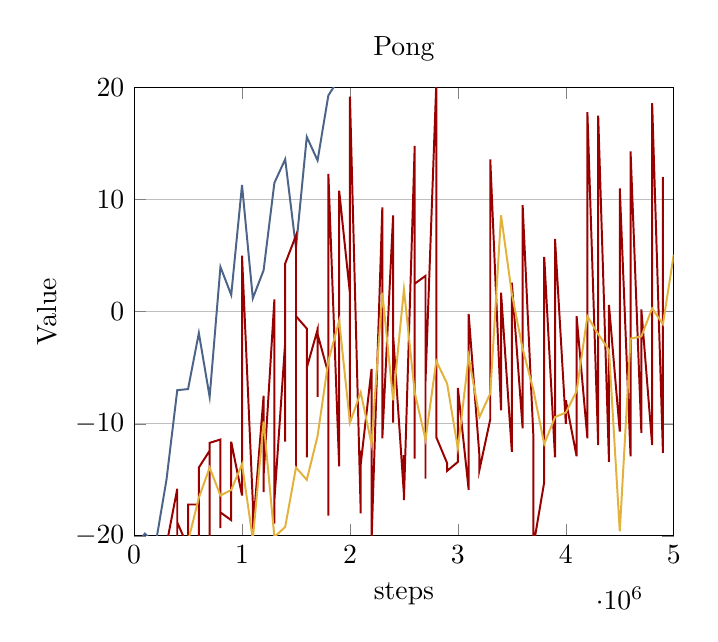
\begin{tikzpicture}

\begin{axis}[%
title=Pong,
% %width=4.634in,
%width=10in,
%height=5in,
%at={(2.596in,2.358in)},
% scale only axis,
xmin=0,
xmax=5000000,
xlabel style={font=\color{white!15!black}},
xlabel={steps},
xlabel near ticks,
ymin=-20,
ymax=20,
ylabel style={font=\color{white!15!black}},
ylabel={Value},
ylabel near ticks,
ymajorgrids,
% %scale=0.5,
%scale=0.4,
axis background/.style={fill=white},
%legend style={legend cell align=left, align=left, draw=white!15!black}
]
\addplot [color=blue, line width = 0.25mm]
                table[row sep=crcr]{
                  0 -21.0\\ 
100000 -19.799999237060547\\ 
200000 -20.700000762939453\\ 
300000 -15.0\\ 
400000 -7.0\\ 
500000 -6.900000095367432\\ 
600000 -1.899999976158142\\ 
700000 -7.599999904632568\\ 
800000 4.0\\ 
900000 1.5\\ 
1000000 11.300000190734863\\ 
1100000 1.2000000476837158\\ 
1200000 3.700000047683716\\ 
1300000 11.5\\ 
1400000 13.600000381469727\\ 
1500000 5.699999809265137\\ 
1600000 15.600000381469727\\ 
1700000 13.5\\ 
1800000 19.299999237060547\\ 
1900000 20.799999237060547\\ 
};
\addplot [color=red, line width = 0.25mm]
                table[row sep=crcr]{
                  0 -21.0\\ 
0 -21.0\\ 
0 -21.0\\ 
0 -21.0\\ 
100000 -21.0\\ 
100000 -20.600000381469727\\ 
100000 -21.0\\ 
200000 -20.399999618530273\\ 
200000 -21.0\\ 
200000 -20.799999237060547\\ 
300000 -20.600000381469727\\ 
300000 -20.799999237060547\\ 
300000 -20.799999237060547\\ 
400000 -15.800000190734863\\ 
400000 -20.399999618530273\\ 
400000 -18.799999237060547\\ 
500000 -21.0\\ 
500000 -21.0\\ 
500000 -17.200000762939453\\ 
600000 -17.200000762939453\\ 
600000 -20.600000381469727\\ 
600000 -13.899999618530273\\ 
700000 -12.399999618530273\\ 
700000 -20.100000381469727\\ 
700000 -11.699999809265137\\ 
800000 -11.399999618530273\\ 
800000 -19.299999237060547\\ 
800000 -17.899999618530273\\ 
900000 -18.600000381469727\\ 
900000 -15.699999809265137\\ 
900000 -11.600000381469727\\ 
1000000 -16.399999618530273\\ 
1000000 -16.0\\ 
1000000 5.0\\ 
1100000 -17.0\\ 
1100000 -17.5\\ 
1100000 -19.600000381469727\\ 
1200000 -7.5\\ 
1200000 -16.100000381469727\\ 
1200000 -14.600000381469727\\ 
1300000 1.100000023841858\\ 
1300000 -18.899999618530273\\ 
1300000 -16.799999237060547\\ 
1400000 -2.700000047683716\\ 
1400000 -11.600000381469727\\ 
1400000 4.300000190734863\\ 
1500000 6.800000190734863\\ 
1500000 -13.899999618530273\\ 
1500000 -0.4000000059604645\\ 
1600000 -1.5\\ 
1600000 -13.0\\ 
1600000 -5.0\\ 
1700000 -1.600000023841858\\ 
1700000 -7.599999904632568\\ 
1700000 -2.0\\ 
1800000 -5.5\\ 
1800000 -18.200000762939453\\ 
1800000 12.300000190734863\\ 
1900000 -13.800000190734863\\ 
1900000 -10.0\\ 
1900000 10.800000190734863\\ 
2000000 1.600000023841858\\ 
2000000 -9.899999618530273\\ 
2000000 19.200000762939453\\ 
2100000 -18.0\\ 
2100000 -12.399999618530273\\ 
2100000 -13.600000381469727\\ 
2200000 -5.099999904632568\\ 
2200000 -13.899999618530273\\ 
2200000 -20.5\\ 
2300000 9.300000190734863\\ 
2300000 -8.199999809265137\\ 
2300000 -11.300000190734863\\ 
2400000 8.600000381469727\\ 
2400000 -9.899999618530273\\ 
2400000 -2.0999999046325684\\ 
2500000 -16.299999237060547\\ 
2500000 -12.800000190734863\\ 
2500000 -16.799999237060547\\ 
2600000 14.800000190734863\\ 
2600000 -13.100000381469727\\ 
2600000 2.5\\ 
2700000 3.200000047683716\\ 
2700000 -14.899999618530273\\ 
2700000 -6.199999809265137\\ 
2800000 20.399999618530273\\ 
2800000 -9.800000190734863\\ 
2800000 -11.199999809265137\\ 
2900000 -13.5\\ 
2900000 -14.199999809265137\\ 
3000000 -13.399999618530273\\ 
3000000 -6.800000190734863\\ 
3100000 -15.899999618530273\\ 
3100000 -0.20000000298023224\\ 
3200000 -12.899999618530273\\ 
3200000 -14.100000381469727\\ 
3300000 -9.600000381469727\\ 
3300000 13.600000381469727\\ 
3400000 -8.800000190734863\\ 
3400000 1.7000000476837158\\ 
3500000 -12.5\\ 
3500000 2.5999999046325684\\ 
3600000 -10.399999618530273\\ 
3600000 9.5\\ 
3700000 -11.199999809265137\\ 
3700000 -20.899999618530273\\ 
3800000 -15.199999809265137\\ 
3800000 4.900000095367432\\ 
3900000 -13.0\\ 
3900000 6.5\\ 
4000000 -10.0\\ 
4000000 -7.900000095367432\\ 
4100000 -12.899999618530273\\ 
4100000 -0.4000000059604645\\ 
4200000 -11.300000190734863\\ 
4200000 17.799999237060547\\ 
4300000 -11.899999618530273\\ 
4300000 17.5\\ 
4400000 -13.399999618530273\\ 
4400000 0.6000000238418579\\ 
4500000 -10.699999809265137\\ 
4500000 11.0\\ 
4600000 -12.899999618530273\\ 
4600000 14.300000190734863\\ 
4700000 -10.800000190734863\\ 
4700000 0.20000000298023224\\ 
4800000 -11.899999618530273\\ 
4800000 18.600000381469727\\ 
4900000 -12.600000381469727\\ 
4900000 12.0\\ 
};
\addplot [color=yellow, line width = 0.25mm]
                table[row sep=crcr]{
                  0 -21.0\\ 
0 -21.0\\ 
100000 -21.0\\ 
200000 -21.0\\ 
300000 -20.399999618530273\\ 
400000 -21.0\\ 
500000 -20.5\\ 
600000 -16.600000381469727\\ 
700000 -13.899999618530273\\ 
800000 -16.399999618530273\\ 
900000 -15.899999618530273\\ 
1000000 -13.600000381469727\\ 
1100000 -20.299999237060547\\ 
1200000 -9.800000190734863\\ 
1300000 -20.100000381469727\\ 
1400000 -19.200000762939453\\ 
1500000 -13.899999618530273\\ 
1600000 -15.0\\ 
1700000 -11.100000381469727\\ 
1800000 -4.400000095367432\\ 
1900000 -0.800000011920929\\ 
2000000 -9.899999618530273\\ 
2100000 -7.199999809265137\\ 
2200000 -11.800000190734863\\ 
2300000 1.7000000476837158\\ 
2400000 -7.900000095367432\\ 
2500000 2.0\\ 
2600000 -7.199999809265137\\ 
2700000 -11.399999618530273\\ 
2800000 -4.400000095367432\\ 
2900000 -6.400000095367432\\ 
3000000 -12.199999809265137\\ 
3100000 -4.0\\ 
3200000 -9.399999618530273\\ 
3300000 -7.300000190734863\\ 
3400000 8.600000381469727\\ 
3500000 1.600000023841858\\ 
3600000 -3.299999952316284\\ 
3700000 -7.0\\ 
3800000 -11.800000190734863\\ 
3900000 -9.399999618530273\\ 
4000000 -9.0\\ 
4100000 -7.099999904632568\\ 
4200000 -0.4000000059604645\\ 
4300000 -2.0\\ 
4400000 -3.4000000953674316\\ 
4500000 -19.600000381469727\\ 
4600000 -2.4000000953674316\\ 
4700000 -2.200000047683716\\ 
4800000 0.30000001192092896\\ 
4900000 -1.100000023841858\\ 
5000000 5.099999904632568\\ 
};
\end{axis}
\end{tikzpicture}}}\\
  \vspace{-1cm}
    \subfloat[]{  \resizebox{0.4\textwidth}{!}{
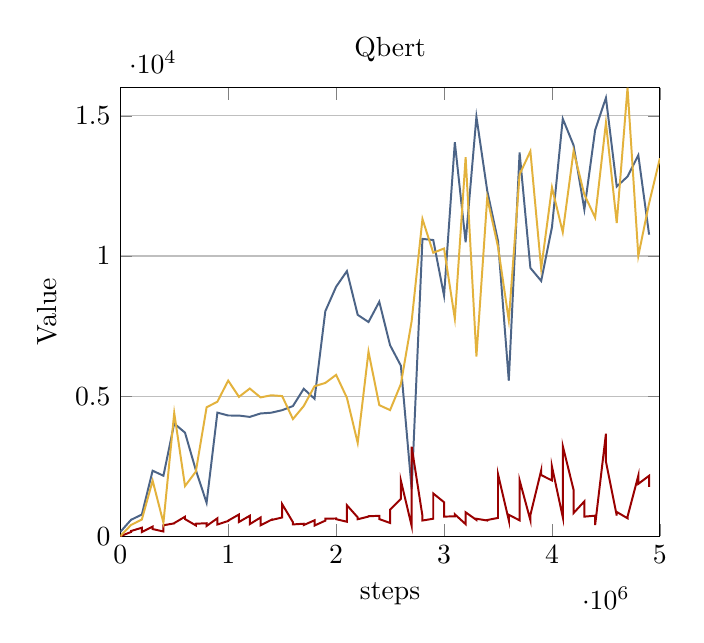
\begin{tikzpicture}

\begin{axis}[%
title=Qbert,
% %width=4.634in,
%width=10in,
%height=5in,
%at={(2.596in,2.358in)},
% scale only axis,
xmin=0,
xmax=5000000,
xlabel style={font=\color{white!15!black}},
xlabel={steps},
xlabel near ticks,
ymin=0,
ymax=16000,
ylabel style={font=\color{white!15!black}},
ylabel={Value},
ylabel near ticks,
ymajorgrids,
% %scale=0.5,
%scale=0.4,
axis background/.style={fill=white},
%legend style={legend cell align=left, align=left, draw=white!15!black}
]
\addplot [color=blue, line width = 0.25mm]
                table[row sep=crcr]{
                  0 150.0\\ 
100000 585.0\\ 
200000 772.5\\ 
300000 2337.5\\ 
400000 2157.5\\ 
500000 4022.5\\ 
600000 3695.0\\ 
700000 2362.5\\ 
800000 1192.5\\ 
900000 4410.0\\ 
1000000 4307.5\\ 
1100000 4305.0\\ 
1200000 4257.5\\ 
1300000 4380.0\\ 
1400000 4407.5\\ 
1500000 4497.5\\ 
1600000 4645.0\\ 
1700000 5260.0\\ 
1800000 4905.0\\ 
1900000 8030.0\\ 
2000000 8902.5\\ 
2100000 9460.0\\ 
2200000 7900.0\\ 
2300000 7642.5\\ 
2400000 8367.5\\ 
2500000 6815.0\\ 
2600000 6085.0\\ 
2700000 1677.5\\ 
2800000 10610.0\\ 
2900000 10570.0\\ 
3000000 8585.0\\ 
3100000 14057.5\\ 
3200000 10490.0\\ 
3300000 14970.0\\ 
3400000 12332.5\\ 
3500000 10537.5\\ 
3600000 5550.0\\ 
3700000 13692.5\\ 
3800000 9572.5\\ 
3900000 9110.0\\ 
4000000 11030.0\\ 
4100000 14897.5\\ 
4200000 13955.0\\ 
4300000 11660.0\\ 
4400000 14495.0\\ 
4500000 15645.0\\ 
4600000 12480.0\\ 
4700000 12835.0\\ 
4800000 13597.5\\ 
4900000 10762.5\\ 
};
\addplot [color=red, line width = 0.25mm]
                table[row sep=crcr]{
                  0 0.0\\ 
0 0.0\\ 
100000 150.0\\ 
100000 185.0\\ 
200000 302.5\\ 
200000 150.0\\ 
300000 342.5\\ 
300000 255.0\\ 
400000 167.5\\ 
400000 390.0\\ 
500000 457.5\\ 
500000 467.5\\ 
600000 695.0\\ 
600000 610.0\\ 
700000 385.0\\ 
700000 445.0\\ 
800000 462.5\\ 
800000 365.0\\ 
900000 640.0\\ 
900000 417.5\\ 
1000000 542.5\\ 
1000000 555.0\\ 
1100000 775.0\\ 
1100000 507.5\\ 
1200000 730.0\\ 
1200000 430.0\\ 
1300000 667.5\\ 
1300000 387.5\\ 
1400000 585.0\\ 
1400000 577.5\\ 
1500000 667.5\\ 
1500000 1145.0\\ 
1600000 500.0\\ 
1600000 420.0\\ 
1700000 445.0\\ 
1700000 397.5\\ 
1800000 567.5\\ 
1800000 380.0\\ 
1900000 555.0\\ 
1900000 625.0\\ 
2000000 632.5\\ 
2000000 607.5\\ 
2100000 515.0\\ 
2100000 1105.0\\ 
2200000 672.5\\ 
2200000 605.0\\ 
2300000 700.0\\ 
2300000 712.5\\ 
2400000 727.5\\ 
2400000 610.0\\ 
2500000 472.5\\ 
2500000 947.5\\ 
2600000 1330.0\\ 
2600000 1985.0\\ 
2700000 365.0\\ 
2700000 3195.0\\ 
2800000 720.0\\ 
2800000 560.0\\ 
2900000 622.5\\ 
2900000 1525.0\\ 
3000000 1212.5\\ 
3000000 700.0\\ 
3100000 707.5\\ 
3100000 780.0\\ 
3200000 430.0\\ 
3200000 852.5\\ 
3300000 580.0\\ 
3300000 622.5\\ 
3400000 560.0\\ 
3400000 577.5\\ 
3500000 652.5\\ 
3500000 2215.0\\ 
3600000 567.5\\ 
3600000 765.0\\ 
3700000 565.0\\ 
3700000 1995.0\\ 
3800000 570.0\\ 
3800000 757.5\\ 
3900000 2345.0\\ 
3900000 2182.5\\ 
4000000 1987.5\\ 
4000000 2482.5\\ 
4100000 682.5\\ 
4100000 3220.0\\ 
4200000 1657.5\\ 
4200000 825.0\\ 
4300000 1242.5\\ 
4300000 697.5\\ 
4400000 732.5\\ 
4400000 397.5\\ 
4500000 3660.0\\ 
4500000 2662.5\\ 
4600000 735.0\\ 
4600000 865.0\\ 
4700000 640.0\\ 
4700000 695.0\\ 
4800000 2160.0\\ 
4800000 1867.5\\ 
4900000 2157.5\\ 
4900000 1762.5\\ 
};
\addplot [color=yellow, line width = 0.25mm]
                table[row sep=crcr]{
                  0 0.0\\ 
0 0.0\\ 
0 0.0\\ 
0 0.0\\ 
100000 400.0\\ 
200000 595.0\\ 
300000 1982.5\\ 
400000 480.0\\ 
500000 4397.5\\ 
600000 1790.0\\ 
700000 2302.5\\ 
800000 4600.0\\ 
900000 4800.0\\ 
1000000 5552.5\\ 
1100000 4972.5\\ 
1200000 5270.0\\ 
1300000 4952.5\\ 
1400000 5030.0\\ 
1500000 5000.0\\ 
1600000 4180.0\\ 
1700000 4645.0\\ 
1800000 5352.5\\ 
1900000 5470.0\\ 
2000000 5757.5\\ 
2100000 4940.0\\ 
2200000 3327.5\\ 
2300000 6585.0\\ 
2400000 4677.5\\ 
2500000 4500.0\\ 
2600000 5430.0\\ 
2700000 7677.5\\ 
2800000 11320.0\\ 
2900000 10115.0\\ 
3000000 10267.5\\ 
3100000 7765.0\\ 
3200000 13525.0\\ 
3300000 6415.0\\ 
3400000 12077.5\\ 
3500000 10327.5\\ 
3600000 7700.0\\ 
3700000 12912.5\\ 
3800000 13737.5\\ 
3900000 9552.5\\ 
4000000 12445.0\\ 
4100000 10847.5\\ 
4200000 13737.5\\ 
4300000 12195.0\\ 
4400000 11370.0\\ 
4500000 14755.0\\ 
4600000 11175.0\\ 
4700000 16002.5\\ 
4800000 10005.0\\ 
4900000 11885.0\\ 
5000000 13490.0\\ 
};
\end{axis}
\end{tikzpicture}}}
    \subfloat[]{  \resizebox{0.4\textwidth}{!}{
\definecolor{blue}{RGB}{76,100,135}
\definecolor{red}{RGB}{153,0,0}
\definecolor{yellow}{RGB}{227,178,60}
\definecolor{mycolor1}{rgb}{0.00000,0.44700,0.74100}%
\definecolor{mycolor2}{rgb}{0.85000,0.32500,0.09800}%
\definecolor{mycolor3}{rgb}{0.92900,0.69400,0.12500}%
%
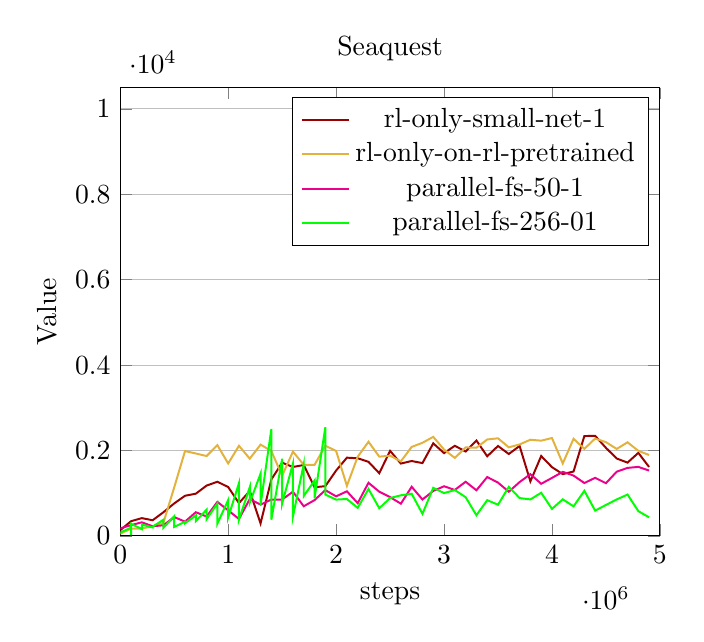
\begin{tikzpicture}

\begin{axis}[%
title=Seaquest,
% %width=4.634in,
%width=10in,
%height=5in,
%at={(2.596in,2.358in)},
% scale only axis,
xmin=0,
xmax=5000000,
xlabel style={font=\color{white!15!black}},
xlabel={steps},
xlabel near ticks,
ymin=0,
ymax=10500,
ylabel style={font=\color{white!15!black}},
ylabel={Value},
ylabel near ticks,
ymajorgrids,
% %scale=0.5,
%scale=0.4,
axis background/.style={fill=white},
%legend style={legend cell align=left, align=left, draw=white!15!black}
]
\addplot [color=red, line width = 0.25mm]
                table[row sep=crcr]{
                  0 134.0\\ 
100000 344.0\\ 
200000 416.0\\ 
300000 366.0\\ 
400000 554.0\\ 
500000 760.0\\ 
600000 940.0\\ 
700000 988.0\\ 
800000 1178.0\\ 
900000 1268.0\\ 
1000000 1144.0\\ 
1100000 768.0\\ 
1200000 1052.0\\ 
1300000 292.0\\ 
1400000 1322.0\\ 
1500000 1714.0\\ 
1600000 1614.0\\ 
1700000 1660.0\\ 
1800000 1140.0\\ 
1900000 1164.0\\ 
2000000 1530.0\\ 
2100000 1832.0\\ 
2200000 1818.0\\ 
2300000 1734.0\\ 
2400000 1468.0\\ 
2500000 1992.0\\ 
2600000 1694.0\\ 
2700000 1754.0\\ 
2800000 1704.0\\ 
2900000 2168.0\\ 
3000000 1938.0\\ 
3100000 2110.0\\ 
3200000 1976.0\\ 
3300000 2234.0\\ 
3400000 1864.0\\ 
3500000 2106.0\\ 
3600000 1918.0\\ 
3700000 2106.0\\ 
3800000 1276.0\\ 
3900000 1870.0\\ 
4000000 1610.0\\ 
4100000 1446.0\\ 
4200000 1508.0\\ 
4300000 2338.0\\ 
4400000 2344.0\\ 
4500000 2062.0\\ 
4600000 1812.0\\ 
4700000 1716.0\\ 
4800000 1944.0\\ 
4900000 1614.0\\ 
};
\addlegendentry{rl-only-small-net-1}
\addplot [color=yellow, line width = 0.25mm]
                table[row sep=crcr]{
                  0 48.0\\ 
100000 172.0\\ 
200000 172.0\\ 
300000 224.0\\ 
400000 308.0\\ 
500000 1136.0\\ 
600000 1986.0\\ 
700000 1930.0\\ 
800000 1870.0\\ 
900000 2124.0\\ 
1000000 1696.0\\ 
1100000 2110.0\\ 
1200000 1808.0\\ 
1300000 2138.0\\ 
1400000 1988.0\\ 
1500000 1408.0\\ 
1600000 1974.0\\ 
1700000 1664.0\\ 
1800000 1662.0\\ 
1900000 2112.0\\ 
2000000 1990.0\\ 
2100000 1172.0\\ 
2200000 1854.0\\ 
2300000 2204.0\\ 
2400000 1856.0\\ 
2500000 1878.0\\ 
2600000 1746.0\\ 
2700000 2084.0\\ 
2800000 2180.0\\ 
2900000 2320.0\\ 
3000000 2022.0\\ 
3100000 1826.0\\ 
3200000 2072.0\\ 
3300000 2064.0\\ 
3400000 2258.0\\ 
3500000 2286.0\\ 
3600000 2074.0\\ 
3700000 2142.0\\ 
3800000 2252.0\\ 
3900000 2230.0\\ 
4000000 2292.0\\ 
4100000 1696.0\\ 
4200000 2274.0\\ 
4300000 2038.0\\ 
4400000 2280.0\\ 
4500000 2196.0\\ 
4600000 2036.0\\ 
4700000 2192.0\\ 
4800000 1992.0\\ 
4900000 1894.0\\ 
};
\addlegendentry{rl-only-on-rl-pretrained}
\addplot [color=magenta, line width = 0.25mm]
                table[row sep=crcr]{
                  0 176.0\\ 
0 176.0\\ 
100000 252.0\\ 
200000 318.0\\ 
300000 226.0\\ 
400000 248.0\\ 
500000 440.0\\ 
600000 334.0\\ 
700000 554.0\\ 
800000 454.0\\ 
900000 796.0\\ 
1000000 598.0\\ 
1100000 396.0\\ 
1200000 862.0\\ 
1300000 732.0\\ 
1400000 850.0\\ 
1500000 852.0\\ 
1600000 1034.0\\ 
1700000 694.0\\ 
1800000 838.0\\ 
1900000 1072.0\\ 
2000000 926.0\\ 
2100000 1044.0\\ 
2200000 766.0\\ 
2300000 1244.0\\ 
2400000 1034.0\\ 
2500000 908.0\\ 
2600000 754.0\\ 
2700000 1150.0\\ 
2800000 852.0\\ 
2900000 1052.0\\ 
3000000 1162.0\\ 
3100000 1076.0\\ 
3200000 1268.0\\ 
3300000 1068.0\\ 
3400000 1378.0\\ 
3500000 1248.0\\ 
3600000 1034.0\\ 
3700000 1260.0\\ 
3800000 1446.0\\ 
3900000 1220.0\\ 
4000000 1358.0\\ 
4100000 1500.0\\ 
4200000 1412.0\\ 
4300000 1238.0\\ 
4400000 1360.0\\ 
4500000 1234.0\\ 
4600000 1504.0\\ 
4700000 1592.0\\ 
4800000 1616.0\\ 
4900000 1530.0\\ 
};
\addlegendentry{parallel-fs-50-1}
\addplot [color=green, line width = 0.25mm]
                table[row sep=crcr]{
                  0 80.0\\ 
0 80.0\\ 
0 80.0\\ 
100000 192.0\\ 
100000 20.0\\ 
100000 284.0\\ 
200000 158.0\\ 
200000 264.0\\ 
300000 198.0\\ 
300000 216.0\\ 
400000 378.0\\ 
400000 192.0\\ 
500000 460.0\\ 
500000 210.0\\ 
600000 330.0\\ 
600000 296.0\\ 
700000 478.0\\ 
700000 344.0\\ 
800000 614.0\\ 
800000 390.0\\ 
900000 758.0\\ 
900000 288.0\\ 
1000000 840.0\\ 
1000000 432.0\\ 
1100000 1236.0\\ 
1100000 384.0\\ 
1200000 1142.0\\ 
1200000 776.0\\ 
1300000 1458.0\\ 
1300000 730.0\\ 
1400000 2504.0\\ 
1400000 380.0\\ 
1500000 1806.0\\ 
1500000 756.0\\ 
1600000 1695.0\\ 
1600000 454.0\\ 
1700000 1678.0\\ 
1700000 932.0\\ 
1800000 1296.0\\ 
1800000 878.0\\ 
1900000 2544.0\\ 
1900000 968.0\\ 
2000000 850.0\\ 
2100000 864.0\\ 
2200000 656.0\\ 
2300000 1098.0\\ 
2400000 648.0\\ 
2500000 886.0\\ 
2600000 950.0\\ 
2700000 988.0\\ 
2800000 516.0\\ 
2900000 1126.0\\ 
3000000 1002.0\\ 
3100000 1074.0\\ 
3200000 906.0\\ 
3300000 484.0\\ 
3400000 836.0\\ 
3500000 730.0\\ 
3600000 1148.0\\ 
3700000 886.0\\ 
3800000 854.0\\ 
3900000 1010.0\\ 
4000000 632.0\\ 
4100000 856.0\\ 
4200000 692.0\\ 
4300000 1056.0\\ 
4400000 592.0\\ 
4500000 724.0\\ 
4600000 854.0\\ 
4700000 968.0\\ 
4800000 580.0\\ 
4900000 434.0\\ 
};
\addlegendentry{parallel-fs-256-01}
\end{axis}
\end{tikzpicture}}}\\
  \vspace{-1cm}
    \subfloat[]{  \resizebox{0.4\textwidth}{!}{
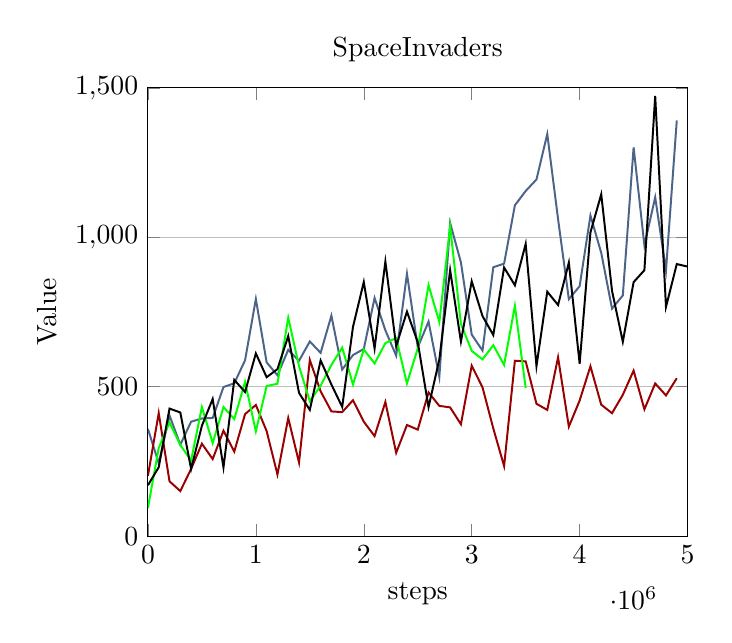
\begin{tikzpicture}

\begin{axis}[%
title=SpaceInvaders,
%width=10in,
%height=5in,
%at={(2.596in,2.358in)},
% scale only axis,
xmin=0,
xmax=5000000,
xlabel style={font=\color{white!15!black}},
xlabel={steps},
xlabel near ticks,
ymin=0,
ymax=1500,
ylabel style={font=\color{white!15!black}},
ylabel={Value},
ylabel near ticks,
ymajorgrids,
% %scale=0.5,
%scale=0.4,
axis background/.style={fill=white},
%legend style={legend cell align=left, align=left, draw=white!15!black}
]
\addplot [color=blue, line width = 0.25mm]
                table[row sep=crcr]{
                  0 359.0\\ 
100000 244.0\\ 
200000 404.0\\ 
300000 306.0\\ 
400000 383.0\\ 
500000 394.0\\ 
600000 395.5\\ 
700000 499.0\\ 
800000 511.5\\ 
900000 588.5\\ 
1000000 793.5\\ 
1100000 581.5\\ 
1200000 538.5\\ 
1300000 623.5\\ 
1400000 587.0\\ 
1500000 651.5\\ 
1600000 613.5\\ 
1700000 738.0\\ 
1800000 557.5\\ 
1900000 606.0\\ 
2000000 626.5\\ 
2100000 797.0\\ 
2200000 689.0\\ 
2300000 604.0\\ 
2400000 878.0\\ 
2500000 632.0\\ 
2600000 718.0\\ 
2700000 533.0\\ 
2800000 1048.0\\ 
2900000 916.0\\ 
3000000 674.5\\ 
3100000 621.0\\ 
3200000 900.0\\ 
3300000 912.0\\ 
3400000 1107.0\\ 
3500000 1155.0\\ 
3600000 1193.5\\ 
3700000 1345.5\\ 
3800000 1061.0\\ 
3900000 793.0\\ 
4000000 836.5\\ 
4100000 1073.0\\ 
4200000 948.0\\ 
4300000 761.5\\ 
4400000 805.5\\ 
4500000 1301.0\\ 
4600000 973.0\\ 
4700000 1134.0\\ 
4800000 889.5\\ 
4900000 1391.0\\ 
};
\addplot [color=red, line width = 0.25mm]
                table[row sep=crcr]{
                  0 202.0\\ 
100000 412.0\\ 
200000 183.5\\ 
300000 151.0\\ 
400000 225.0\\ 
500000 309.5\\ 
600000 258.0\\ 
700000 353.0\\ 
800000 283.0\\ 
900000 408.5\\ 
1000000 439.0\\ 
1100000 351.5\\ 
1200000 206.5\\ 
1300000 395.5\\ 
1400000 246.5\\ 
1500000 589.5\\ 
1600000 485.0\\ 
1700000 417.5\\ 
1800000 415.0\\ 
1900000 455.0\\ 
2000000 383.0\\ 
2100000 335.0\\ 
2200000 449.0\\ 
2300000 279.0\\ 
2400000 372.0\\ 
2500000 356.5\\ 
2600000 481.0\\ 
2700000 436.0\\ 
2800000 431.0\\ 
2900000 374.5\\ 
3000000 570.5\\ 
3100000 498.0\\ 
3200000 360.5\\ 
3300000 234.5\\ 
3400000 587.0\\ 
3500000 585.0\\ 
3600000 443.0\\ 
3700000 422.5\\ 
3800000 598.5\\ 
3900000 366.5\\ 
4000000 454.0\\ 
4100000 568.5\\ 
4200000 440.0\\ 
4300000 411.5\\ 
4400000 473.0\\ 
4500000 554.0\\ 
4600000 424.5\\ 
4700000 511.0\\ 
4800000 471.0\\ 
4900000 528.5\\ 
};
\addplot [color=green, line width = 0.25mm]
                table[row sep=crcr]{
                  0 94.5\\ 
100000 295.0\\ 
200000 380.5\\ 
300000 305.0\\ 
400000 253.0\\ 
500000 432.0\\ 
600000 311.5\\ 
700000 432.0\\ 
800000 392.0\\ 
900000 516.0\\ 
1000000 351.0\\ 
1100000 502.5\\ 
1200000 510.0\\ 
1300000 731.0\\ 
1400000 569.0\\ 
1500000 451.5\\ 
1600000 503.5\\ 
1700000 573.0\\ 
1800000 631.0\\ 
1900000 507.5\\ 
2000000 624.5\\ 
2100000 578.0\\ 
2200000 646.0\\ 
2300000 663.0\\ 
2400000 511.0\\ 
2500000 628.0\\ 
2600000 840.0\\ 
2700000 716.5\\ 
2800000 1037.0\\ 
2900000 710.5\\ 
3000000 620.0\\ 
3100000 591.5\\ 
3200000 639.0\\ 
3300000 573.0\\ 
3400000 771.0\\ 
3500000 496.0\\ 
};
\addplot [color=black, line width = 0.25mm]
                table[row sep=crcr]{
                  0 170.5\\ 
100000 230.5\\ 
200000 427.0\\ 
300000 414.0\\ 
400000 225.0\\ 
500000 369.5\\ 
600000 459.0\\ 
700000 230.0\\ 
800000 523.0\\ 
900000 482.5\\ 
1000000 611.5\\ 
1100000 532.0\\ 
1200000 559.0\\ 
1300000 669.5\\ 
1400000 479.5\\ 
1500000 422.5\\ 
1600000 588.0\\ 
1700000 507.5\\ 
1800000 432.5\\ 
1900000 700.5\\ 
2000000 850.5\\ 
2100000 628.0\\ 
2200000 919.0\\ 
2300000 636.0\\ 
2400000 751.5\\ 
2500000 649.0\\ 
2600000 432.0\\ 
2700000 591.5\\ 
2800000 890.0\\ 
2900000 651.0\\ 
3000000 853.0\\ 
3100000 736.5\\ 
3200000 673.0\\ 
3300000 899.0\\ 
3400000 839.5\\ 
3500000 978.0\\ 
3600000 569.0\\ 
3700000 818.0\\ 
3800000 773.5\\ 
3900000 915.5\\ 
4000000 577.0\\ 
4100000 1016.5\\ 
4200000 1144.0\\ 
4300000 821.0\\ 
4400000 650.5\\ 
4500000 850.0\\ 
4600000 890.0\\ 
4700000 1473.0\\ 
4800000 767.0\\ 
4900000 910.5\\ 
5000000 902.0\\ 
};
\end{axis}
\end{tikzpicture}}}
  \\

  \ref{named}
  \caption{Comparison between latent representation trained to compress the current frames and 
  those trained to perform one-step forward predictions. Despite having a significantly higher reconstruction error,
encoder trained to perform forward prediction perform better.}
  \label{fig:forward-vs-compression}
\end{figure}


Despite fairly poor reconstruction capabilities and an error larger by an order of magnitude, 
state representation trained with forward 
prediction are overall more effective than simple compression.
As with all results, the effects vary from game to game.


%++++++++++++++++++++++++++++
%TEST
%++++++++++++++++++++++++++
%
%\begin{figure}[!t]
%  \captionsetup[subfloat]{position=top,labelformat=empty}
%  \centering
%
%    \subfloat[]{  \resizebox{0.4\textwidth}{!}{
%\definecolor{blue}{RGB}{76,100,135}
%\definecolor{red}{RGB}{153,0,0}
%\definecolor{yellow}{RGB}{227,178,60}
%\definecolor{mycolor1}{rgb}{0.00000,0.44700,0.74100}%
%\definecolor{mycolor2}{rgb}{0.85000,0.32500,0.09800}%
%\definecolor{mycolor3}{rgb}{0.92900,0.69400,0.12500}%
%
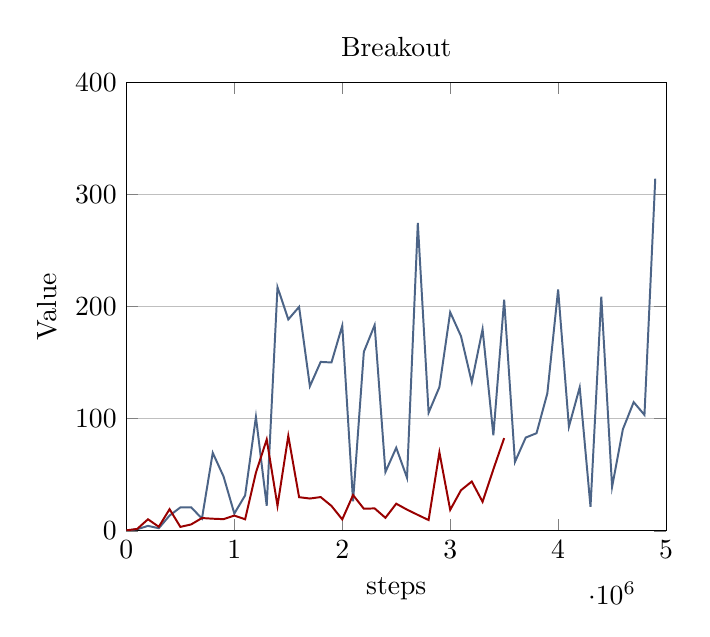
\begin{tikzpicture}

\begin{axis}[%
legend entries={rl-only-small-net,L2-reg,parallel-fs-50-no-aug}, 
legend columns=2,
title=Breakout,
legend to name=named,
legend style={legend cell align=left},
%%width=10in,
%%height=5in,
%%at={(2.596in,2.358in)},
% scale only axis,
xmin=0,
xmax=5000000,
xlabel style={font=\color{white!15!black}},
xlabel={steps},
xlabel near ticks,
ymin=0,
ymax=400,
ylabel style={font=\color{white!15!black}},
ylabel={Value},
ylabel near ticks,
ymajorgrids,
% %scale=0.5,
%%scale=0.4,
axis background/.style={fill=white},
%legend columns=2,
%legend=south outside
]
\addplot [color=blue, line width = 0.25mm]
                table[row sep=crcr]{
                  0 0.20000000298023224\\ 
100000 1.399999976158142\\ 
200000 4.400000095367432\\ 
300000 2.299999952316284\\ 
400000 13.600000381469727\\ 
500000 20.899999618530273\\ 
600000 21.0\\ 
700000 10.899999618530273\\ 
800000 69.5999984741211\\ 
900000 48.5\\ 
1000000 15.399999618530273\\ 
1100000 31.600000381469727\\ 
1200000 101.5999984741211\\ 
1300000 22.399999618530273\\ 
1400000 217.39999389648438\\ 
1500000 188.60000610351562\\ 
1600000 199.8000030517578\\ 
1700000 129.0\\ 
1800000 150.6999969482422\\ 
1900000 150.1999969482422\\ 
2000000 183.0\\ 
2100000 26.399999618530273\\ 
2200000 159.6999969482422\\ 
2300000 183.5\\ 
2400000 52.5\\ 
2500000 74.0999984741211\\ 
2600000 47.29999923706055\\ 
2700000 274.6000061035156\\ 
2800000 105.4000015258789\\ 
2900000 128.1999969482422\\ 
3000000 195.0\\ 
3100000 173.6999969482422\\ 
3200000 132.60000610351562\\ 
3300000 179.89999389648438\\ 
3400000 85.19999694824219\\ 
3500000 206.1999969482422\\ 
3600000 61.5\\ 
3700000 83.19999694824219\\ 
3800000 87.0999984741211\\ 
3900000 122.5999984741211\\ 
4000000 215.3000030517578\\ 
4100000 92.9000015258789\\ 
4200000 128.0\\ 
4300000 21.399999618530273\\ 
4400000 208.89999389648438\\ 
4500000 39.20000076293945\\ 
4600000 90.5999984741211\\ 
4700000 114.80000305175781\\ 
4800000 103.4000015258789\\ 
4900000 314.20001220703125\\ 
};
\addplot [color=red, line width = 0.25mm]
                table[row sep=crcr]{
                  0 0.4000000059604645\\ 
100000 1.7000000476837158\\ 
200000 10.300000190734863\\ 
300000 3.5999999046325684\\ 
400000 19.299999237060547\\ 
500000 3.5\\ 
600000 5.699999809265137\\ 
700000 11.399999618530273\\ 
800000 10.800000190734863\\ 
900000 10.399999618530273\\ 
1000000 13.600000381469727\\ 
1100000 10.300000190734863\\ 
1200000 51.900001525878906\\ 
1300000 81.5\\ 
1400000 22.299999237060547\\ 
1500000 84.69999694824219\\ 
1600000 30.0\\ 
1700000 28.799999237060547\\ 
1800000 30.100000381469727\\ 
1900000 22.200000762939453\\ 
2000000 10.199999809265137\\ 
2100000 31.899999618530273\\ 
2200000 19.700000762939453\\ 
2300000 20.0\\ 
2400000 11.600000381469727\\ 
2500000 24.200000762939453\\ 
2600000 18.899999618530273\\ 
2700000 14.199999809265137\\ 
2800000 9.600000381469727\\ 
2900000 70.0\\ 
3000000 18.700000762939453\\ 
3100000 36.20000076293945\\ 
3200000 44.0\\ 
3300000 25.899999618530273\\ 
3400000 54.900001525878906\\ 
3500000 82.69999694824219\\ 
};
\addplot [color=yellow, line width = 0.25mm]
                table[row sep=crcr]{
                  0 0.800000011920929\\ 
};
\end{axis}
\end{tikzpicture}}}
%    \subfloat[]{  \resizebox{0.4\textwidth}{!}{
%\definecolor{blue}{RGB}{76,100,135}
%\definecolor{red}{RGB}{153,0,0}
%\definecolor{yellow}{RGB}{227,178,60}
%\definecolor{mycolor1}{rgb}{0.00000,0.44700,0.74100}%
%\definecolor{mycolor2}{rgb}{0.85000,0.32500,0.09800}%
%\definecolor{mycolor3}{rgb}{0.92900,0.69400,0.12500}%
%
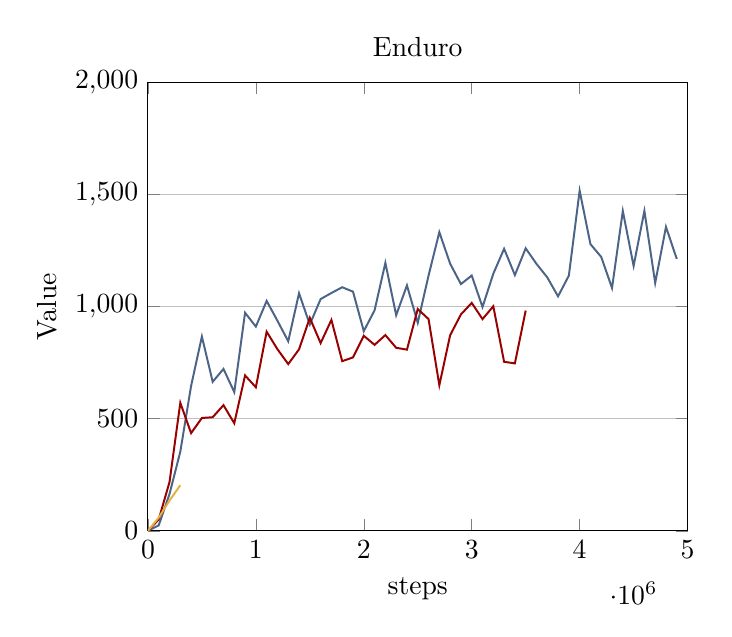
\begin{tikzpicture}

\begin{axis}[%
title=Enduro,
% %width=4.634in,
%%width=10in,
%%height=5in,
%at={(2.596in,2.358in)},
% scale only axis,
xmin=0,
xmax=5000000,
xlabel style={font=\color{white!15!black}},
xlabel={steps},
xlabel near ticks,
ymin=0,
ymax=2000,
ylabel style={font=\color{white!15!black}},
ylabel={Value},
ylabel near ticks,
ymajorgrids,
% %scale=0.5,
%scale=0.4,
axis background/.style={fill=white},
%legend style={legend cell align=left, align=left, draw=white!15!black}
]
\addplot [color=blue, line width = 0.25mm]
                table[row sep=crcr]{
                  0 0.0\\ 
100000 24.299999237060547\\ 
200000 164.3000030517578\\ 
300000 353.0\\ 
400000 646.4000244140625\\ 
500000 866.7000122070312\\ 
600000 664.7000122070312\\ 
700000 722.2000122070312\\ 
800000 618.9000244140625\\ 
900000 972.7999877929688\\ 
1000000 910.9000244140625\\ 
1100000 1025.699951171875\\ 
1200000 937.0\\ 
1300000 845.5999755859375\\ 
1400000 1059.9000244140625\\ 
1500000 920.2999877929688\\ 
1600000 1033.800048828125\\ 
1700000 1061.0\\ 
1800000 1086.5999755859375\\ 
1900000 1066.9000244140625\\ 
2000000 890.9000244140625\\ 
2100000 983.5\\ 
2200000 1195.300048828125\\ 
2300000 962.0\\ 
2400000 1094.800048828125\\ 
2500000 928.0\\ 
2600000 1138.5999755859375\\ 
2700000 1332.300048828125\\ 
2800000 1191.800048828125\\ 
2900000 1100.5999755859375\\ 
3000000 1138.800048828125\\ 
3100000 998.2999877929688\\ 
3200000 1146.800048828125\\ 
3300000 1258.0999755859375\\ 
3400000 1141.0\\ 
3500000 1260.300048828125\\ 
3600000 1190.800048828125\\ 
3700000 1130.5999755859375\\ 
3800000 1046.0999755859375\\ 
3900000 1138.4000244140625\\ 
4000000 1517.5\\ 
4100000 1278.9000244140625\\ 
4200000 1221.699951171875\\ 
4300000 1083.199951171875\\ 
4400000 1426.9000244140625\\ 
4500000 1181.5999755859375\\ 
4600000 1427.199951171875\\ 
4700000 1105.800048828125\\ 
4800000 1355.800048828125\\ 
4900000 1212.9000244140625\\ 
};
\addplot [color=red, line width = 0.25mm]
                table[row sep=crcr]{
                  0 0.0\\ 
100000 50.5\\ 
200000 217.60000610351562\\ 
300000 570.9000244140625\\ 
400000 435.6000061035156\\ 
500000 503.3999938964844\\ 
600000 506.79998779296875\\ 
700000 560.5\\ 
800000 479.79998779296875\\ 
900000 693.2000122070312\\ 
1000000 640.4000244140625\\ 
1100000 888.4000244140625\\ 
1200000 810.0999755859375\\ 
1300000 743.7999877929688\\ 
1400000 809.5\\ 
1500000 950.2000122070312\\ 
1600000 837.4000244140625\\ 
1700000 940.7999877929688\\ 
1800000 756.7999877929688\\ 
1900000 773.5\\ 
2000000 870.0999755859375\\ 
2100000 829.5999755859375\\ 
2200000 873.2000122070312\\ 
2300000 816.5\\ 
2400000 808.2000122070312\\ 
2500000 989.5999755859375\\ 
2600000 944.5\\ 
2700000 649.4000244140625\\ 
2800000 872.4000244140625\\ 
2900000 965.2000122070312\\ 
3000000 1016.7000122070312\\ 
3100000 944.4000244140625\\ 
3200000 1001.7000122070312\\ 
3300000 754.0\\ 
3400000 746.7999877929688\\ 
3500000 982.2999877929688\\ 
};
\addplot [color=yellow, line width = 0.25mm]
                table[row sep=crcr]{
                  0 0.0\\ 
100000 58.79999923706055\\ 
200000 135.10000610351562\\ 
300000 203.1999969482422\\ 
};
\end{axis}
\end{tikzpicture}}}\\
%  \vspace{-1cm}
%    \subfloat[]{  \resizebox{0.4\textwidth}{!}{
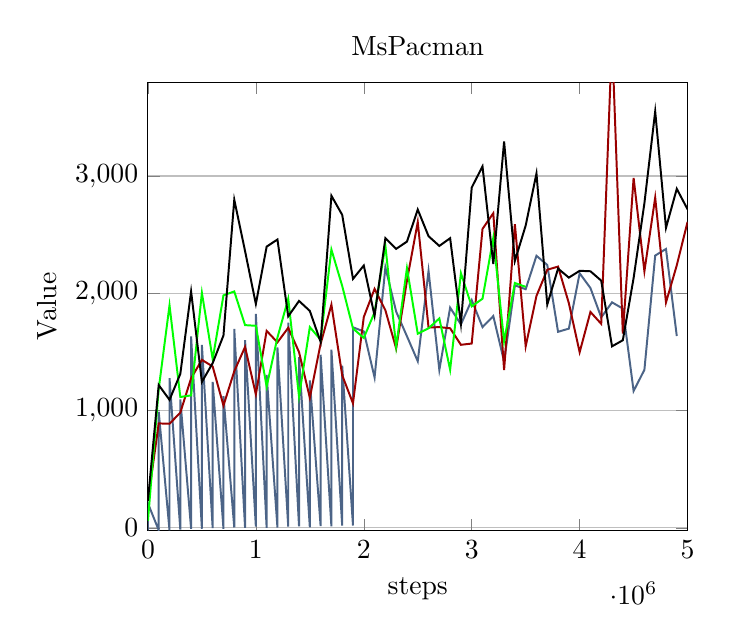
\begin{tikzpicture}

\begin{axis}[%
title=MsPacman,
% %width=4.634in,
%width=10in,
%height=5in,
%at={(2.596in,2.358in)},
% scale only axis,
xmin=0,
xmax=5000000,
xlabel style={font=\color{white!15!black}},
xlabel={steps},
xlabel near ticks,
ymin=-22,
ymax=3800,
ylabel style={font=\color{white!15!black}},
ylabel={Value},
ylabel near ticks,
ymajorgrids,
% %scale=0.5,
%scale=0.4,
axis background/.style={fill=white},
%legend style={legend cell align=left, align=left, draw=white!15!black}
]
\addplot [color=blue, line width = 0.25mm]
                table[row sep=crcr]{
                  0 -21.0\\ 
0 210.0\\ 
100000 -19.799999237060547\\ 
100000 990.0\\ 
200000 -20.700000762939453\\ 
200000 1277.0\\ 
300000 -15.0\\ 
300000 1096.0\\ 
400000 -7.0\\ 
400000 1632.0\\ 
500000 -6.900000095367432\\ 
500000 1561.0\\ 
600000 -1.899999976158142\\ 
600000 1245.0\\ 
700000 -7.599999904632568\\ 
700000 1123.0\\ 
800000 4.0\\ 
800000 1696.0\\ 
900000 1.5\\ 
900000 1600.0\\ 
1000000 11.300000190734863\\ 
1000000 1824.0\\ 
1100000 1.2000000476837158\\ 
1100000 1304.0\\ 
1200000 3.700000047683716\\ 
1200000 1538.0\\ 
1300000 11.5\\ 
1300000 1750.0\\ 
1400000 13.600000381469727\\ 
1400000 1456.0\\ 
1500000 5.699999809265137\\ 
1500000 1258.0\\ 
1600000 15.600000381469727\\ 
1600000 1476.0\\ 
1700000 13.5\\ 
1700000 1519.0\\ 
1800000 19.299999237060547\\ 
1800000 1383.0\\ 
1900000 20.799999237060547\\ 
1900000 1710.0\\ 
2000000 1675.0\\ 
2100000 1282.0\\ 
2200000 2222.0\\ 
2300000 1844.0\\ 
2400000 1634.0\\ 
2500000 1421.0\\ 
2600000 2191.0\\ 
2700000 1347.0\\ 
2800000 1878.0\\ 
2900000 1735.0\\ 
3000000 1942.0\\ 
3100000 1712.0\\ 
3200000 1806.0\\ 
3300000 1419.0\\ 
3400000 2068.0\\ 
3500000 2035.0\\ 
3600000 2320.0\\ 
3700000 2242.0\\ 
3800000 1672.0\\ 
3900000 1699.0\\ 
4000000 2171.0\\ 
4100000 2045.0\\ 
4200000 1795.0\\ 
4300000 1923.0\\ 
4400000 1870.0\\ 
4500000 1167.0\\ 
4600000 1348.0\\ 
4700000 2322.0\\ 
4800000 2378.0\\ 
4900000 1636.0\\ 
};
\addplot [color=red, line width = 0.25mm]
                table[row sep=crcr]{
                  0 230.0\\ 
100000 891.0\\ 
200000 888.0\\ 
300000 983.0\\ 
400000 1276.0\\ 
500000 1433.0\\ 
600000 1376.0\\ 
700000 1043.0\\ 
800000 1336.0\\ 
900000 1543.0\\ 
1000000 1139.0\\ 
1100000 1680.0\\ 
1200000 1582.0\\ 
1300000 1706.0\\ 
1400000 1499.0\\ 
1500000 1110.0\\ 
1600000 1569.0\\ 
1700000 1903.0\\ 
1800000 1301.0\\ 
1900000 1062.0\\ 
2000000 1798.0\\ 
2100000 2038.0\\ 
2200000 1856.0\\ 
2300000 1530.0\\ 
2400000 2109.0\\ 
2500000 2607.0\\ 
2600000 1708.0\\ 
2700000 1712.0\\ 
2800000 1702.0\\ 
2900000 1561.0\\ 
3000000 1572.0\\ 
3100000 2549.0\\ 
3200000 2683.0\\ 
3300000 1346.0\\ 
3400000 2590.0\\ 
3500000 1548.0\\ 
3600000 1978.0\\ 
3700000 2201.0\\ 
3800000 2228.0\\ 
3900000 1916.0\\ 
4000000 1498.0\\ 
4100000 1841.0\\ 
4200000 1740.0\\ 
4300000 4177.0\\ 
4400000 1656.0\\ 
4500000 2984.0\\ 
4600000 2188.0\\ 
4700000 2816.0\\ 
4800000 1922.0\\ 
4900000 2239.0\\ 
5000000 2609.0\\ 
};
\addplot [color=green, line width = 0.25mm]
                table[row sep=crcr]{
                  0 60.0\\ 
100000 1185.0\\ 
200000 1898.0\\ 
300000 1116.0\\ 
400000 1130.0\\ 
500000 2004.0\\ 
600000 1439.0\\ 
700000 1983.0\\ 
800000 2016.0\\ 
900000 1729.0\\ 
1000000 1723.0\\ 
1100000 1205.0\\ 
1200000 1623.0\\ 
1300000 1954.0\\ 
1400000 1121.0\\ 
1500000 1712.0\\ 
1600000 1604.0\\ 
1700000 2373.0\\ 
1800000 2063.0\\ 
1900000 1700.0\\ 
2000000 1620.0\\ 
2100000 1838.0\\ 
2200000 2406.0\\ 
2300000 1546.0\\ 
2400000 2215.0\\ 
2500000 1656.0\\ 
2600000 1702.0\\ 
2700000 1786.0\\ 
2800000 1348.0\\ 
2900000 2172.0\\ 
3000000 1889.0\\ 
3100000 1954.0\\ 
3200000 2473.0\\ 
3300000 1591.0\\ 
3400000 2088.0\\ 
3500000 2055.0\\ 
};
\addplot [color=black, line width = 0.25mm]
                table[row sep=crcr]{
                  0 230.0\\ 
100000 1218.0\\ 
200000 1092.0\\ 
300000 1313.0\\ 
400000 2016.0\\ 
500000 1245.0\\ 
600000 1405.0\\ 
700000 1641.0\\ 
800000 2798.0\\ 
900000 2360.0\\ 
1000000 1909.0\\ 
1100000 2398.0\\ 
1200000 2459.0\\ 
1300000 1804.0\\ 
1400000 1935.0\\ 
1500000 1850.0\\ 
1600000 1586.0\\ 
1700000 2832.0\\ 
1800000 2669.0\\ 
1900000 2123.0\\ 
2000000 2237.0\\ 
2100000 1808.0\\ 
2200000 2470.0\\ 
2300000 2379.0\\ 
2400000 2441.0\\ 
2500000 2714.0\\ 
2600000 2487.0\\ 
2700000 2404.0\\ 
2800000 2470.0\\ 
2900000 1739.0\\ 
3000000 2902.0\\ 
3100000 3082.0\\ 
3200000 2250.0\\ 
3300000 3294.0\\ 
3400000 2276.0\\ 
3500000 2578.0\\ 
3600000 3022.0\\ 
3700000 1904.0\\ 
3800000 2211.0\\ 
3900000 2134.0\\ 
4000000 2192.0\\ 
4100000 2188.0\\ 
4200000 2108.0\\ 
4300000 1548.0\\ 
4400000 1600.0\\ 
4500000 2130.0\\ 
4600000 2768.0\\ 
4700000 3551.0\\ 
4800000 2558.0\\ 
4900000 2891.0\\ 
5000000 2716.0\\ 
};
\end{axis}
\end{tikzpicture}}}
%    \subfloat[]{  \resizebox{0.4\textwidth}{!}{
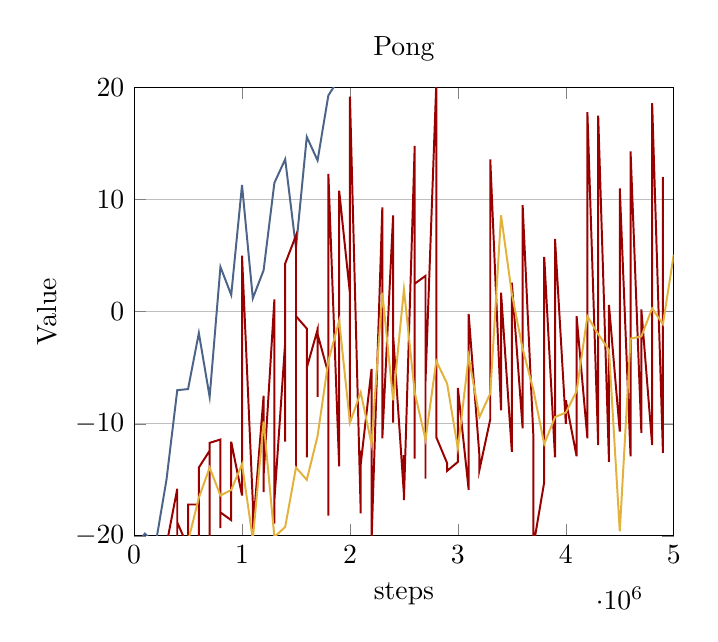
\begin{tikzpicture}

\begin{axis}[%
title=Pong,
% %width=4.634in,
%width=10in,
%height=5in,
%at={(2.596in,2.358in)},
% scale only axis,
xmin=0,
xmax=5000000,
xlabel style={font=\color{white!15!black}},
xlabel={steps},
xlabel near ticks,
ymin=-20,
ymax=20,
ylabel style={font=\color{white!15!black}},
ylabel={Value},
ylabel near ticks,
ymajorgrids,
% %scale=0.5,
%scale=0.4,
axis background/.style={fill=white},
%legend style={legend cell align=left, align=left, draw=white!15!black}
]
\addplot [color=blue, line width = 0.25mm]
                table[row sep=crcr]{
                  0 -21.0\\ 
100000 -19.799999237060547\\ 
200000 -20.700000762939453\\ 
300000 -15.0\\ 
400000 -7.0\\ 
500000 -6.900000095367432\\ 
600000 -1.899999976158142\\ 
700000 -7.599999904632568\\ 
800000 4.0\\ 
900000 1.5\\ 
1000000 11.300000190734863\\ 
1100000 1.2000000476837158\\ 
1200000 3.700000047683716\\ 
1300000 11.5\\ 
1400000 13.600000381469727\\ 
1500000 5.699999809265137\\ 
1600000 15.600000381469727\\ 
1700000 13.5\\ 
1800000 19.299999237060547\\ 
1900000 20.799999237060547\\ 
};
\addplot [color=red, line width = 0.25mm]
                table[row sep=crcr]{
                  0 -21.0\\ 
0 -21.0\\ 
0 -21.0\\ 
0 -21.0\\ 
100000 -21.0\\ 
100000 -20.600000381469727\\ 
100000 -21.0\\ 
200000 -20.399999618530273\\ 
200000 -21.0\\ 
200000 -20.799999237060547\\ 
300000 -20.600000381469727\\ 
300000 -20.799999237060547\\ 
300000 -20.799999237060547\\ 
400000 -15.800000190734863\\ 
400000 -20.399999618530273\\ 
400000 -18.799999237060547\\ 
500000 -21.0\\ 
500000 -21.0\\ 
500000 -17.200000762939453\\ 
600000 -17.200000762939453\\ 
600000 -20.600000381469727\\ 
600000 -13.899999618530273\\ 
700000 -12.399999618530273\\ 
700000 -20.100000381469727\\ 
700000 -11.699999809265137\\ 
800000 -11.399999618530273\\ 
800000 -19.299999237060547\\ 
800000 -17.899999618530273\\ 
900000 -18.600000381469727\\ 
900000 -15.699999809265137\\ 
900000 -11.600000381469727\\ 
1000000 -16.399999618530273\\ 
1000000 -16.0\\ 
1000000 5.0\\ 
1100000 -17.0\\ 
1100000 -17.5\\ 
1100000 -19.600000381469727\\ 
1200000 -7.5\\ 
1200000 -16.100000381469727\\ 
1200000 -14.600000381469727\\ 
1300000 1.100000023841858\\ 
1300000 -18.899999618530273\\ 
1300000 -16.799999237060547\\ 
1400000 -2.700000047683716\\ 
1400000 -11.600000381469727\\ 
1400000 4.300000190734863\\ 
1500000 6.800000190734863\\ 
1500000 -13.899999618530273\\ 
1500000 -0.4000000059604645\\ 
1600000 -1.5\\ 
1600000 -13.0\\ 
1600000 -5.0\\ 
1700000 -1.600000023841858\\ 
1700000 -7.599999904632568\\ 
1700000 -2.0\\ 
1800000 -5.5\\ 
1800000 -18.200000762939453\\ 
1800000 12.300000190734863\\ 
1900000 -13.800000190734863\\ 
1900000 -10.0\\ 
1900000 10.800000190734863\\ 
2000000 1.600000023841858\\ 
2000000 -9.899999618530273\\ 
2000000 19.200000762939453\\ 
2100000 -18.0\\ 
2100000 -12.399999618530273\\ 
2100000 -13.600000381469727\\ 
2200000 -5.099999904632568\\ 
2200000 -13.899999618530273\\ 
2200000 -20.5\\ 
2300000 9.300000190734863\\ 
2300000 -8.199999809265137\\ 
2300000 -11.300000190734863\\ 
2400000 8.600000381469727\\ 
2400000 -9.899999618530273\\ 
2400000 -2.0999999046325684\\ 
2500000 -16.299999237060547\\ 
2500000 -12.800000190734863\\ 
2500000 -16.799999237060547\\ 
2600000 14.800000190734863\\ 
2600000 -13.100000381469727\\ 
2600000 2.5\\ 
2700000 3.200000047683716\\ 
2700000 -14.899999618530273\\ 
2700000 -6.199999809265137\\ 
2800000 20.399999618530273\\ 
2800000 -9.800000190734863\\ 
2800000 -11.199999809265137\\ 
2900000 -13.5\\ 
2900000 -14.199999809265137\\ 
3000000 -13.399999618530273\\ 
3000000 -6.800000190734863\\ 
3100000 -15.899999618530273\\ 
3100000 -0.20000000298023224\\ 
3200000 -12.899999618530273\\ 
3200000 -14.100000381469727\\ 
3300000 -9.600000381469727\\ 
3300000 13.600000381469727\\ 
3400000 -8.800000190734863\\ 
3400000 1.7000000476837158\\ 
3500000 -12.5\\ 
3500000 2.5999999046325684\\ 
3600000 -10.399999618530273\\ 
3600000 9.5\\ 
3700000 -11.199999809265137\\ 
3700000 -20.899999618530273\\ 
3800000 -15.199999809265137\\ 
3800000 4.900000095367432\\ 
3900000 -13.0\\ 
3900000 6.5\\ 
4000000 -10.0\\ 
4000000 -7.900000095367432\\ 
4100000 -12.899999618530273\\ 
4100000 -0.4000000059604645\\ 
4200000 -11.300000190734863\\ 
4200000 17.799999237060547\\ 
4300000 -11.899999618530273\\ 
4300000 17.5\\ 
4400000 -13.399999618530273\\ 
4400000 0.6000000238418579\\ 
4500000 -10.699999809265137\\ 
4500000 11.0\\ 
4600000 -12.899999618530273\\ 
4600000 14.300000190734863\\ 
4700000 -10.800000190734863\\ 
4700000 0.20000000298023224\\ 
4800000 -11.899999618530273\\ 
4800000 18.600000381469727\\ 
4900000 -12.600000381469727\\ 
4900000 12.0\\ 
};
\addplot [color=yellow, line width = 0.25mm]
                table[row sep=crcr]{
                  0 -21.0\\ 
0 -21.0\\ 
100000 -21.0\\ 
200000 -21.0\\ 
300000 -20.399999618530273\\ 
400000 -21.0\\ 
500000 -20.5\\ 
600000 -16.600000381469727\\ 
700000 -13.899999618530273\\ 
800000 -16.399999618530273\\ 
900000 -15.899999618530273\\ 
1000000 -13.600000381469727\\ 
1100000 -20.299999237060547\\ 
1200000 -9.800000190734863\\ 
1300000 -20.100000381469727\\ 
1400000 -19.200000762939453\\ 
1500000 -13.899999618530273\\ 
1600000 -15.0\\ 
1700000 -11.100000381469727\\ 
1800000 -4.400000095367432\\ 
1900000 -0.800000011920929\\ 
2000000 -9.899999618530273\\ 
2100000 -7.199999809265137\\ 
2200000 -11.800000190734863\\ 
2300000 1.7000000476837158\\ 
2400000 -7.900000095367432\\ 
2500000 2.0\\ 
2600000 -7.199999809265137\\ 
2700000 -11.399999618530273\\ 
2800000 -4.400000095367432\\ 
2900000 -6.400000095367432\\ 
3000000 -12.199999809265137\\ 
3100000 -4.0\\ 
3200000 -9.399999618530273\\ 
3300000 -7.300000190734863\\ 
3400000 8.600000381469727\\ 
3500000 1.600000023841858\\ 
3600000 -3.299999952316284\\ 
3700000 -7.0\\ 
3800000 -11.800000190734863\\ 
3900000 -9.399999618530273\\ 
4000000 -9.0\\ 
4100000 -7.099999904632568\\ 
4200000 -0.4000000059604645\\ 
4300000 -2.0\\ 
4400000 -3.4000000953674316\\ 
4500000 -19.600000381469727\\ 
4600000 -2.4000000953674316\\ 
4700000 -2.200000047683716\\ 
4800000 0.30000001192092896\\ 
4900000 -1.100000023841858\\ 
5000000 5.099999904632568\\ 
};
\end{axis}
\end{tikzpicture}}}\\
%  \vspace{-1cm}
%    \subfloat[]{  \resizebox{0.4\textwidth}{!}{
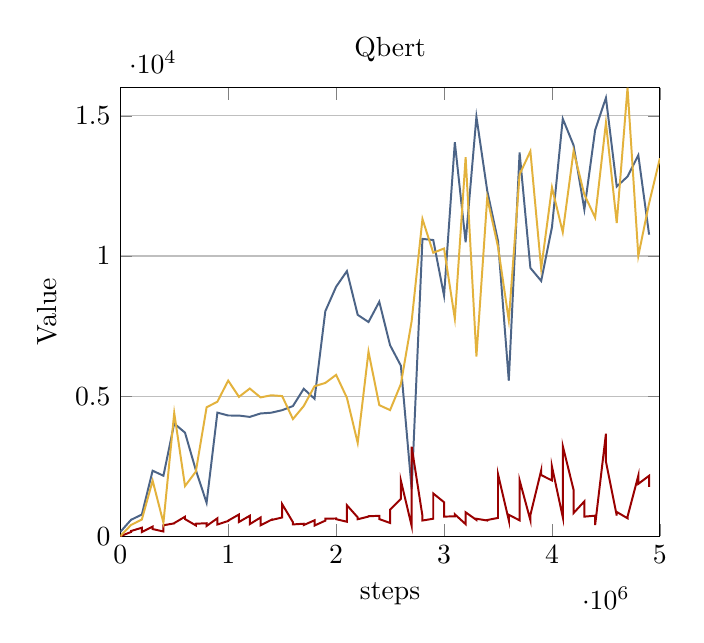
\begin{tikzpicture}

\begin{axis}[%
title=Qbert,
% %width=4.634in,
%width=10in,
%height=5in,
%at={(2.596in,2.358in)},
% scale only axis,
xmin=0,
xmax=5000000,
xlabel style={font=\color{white!15!black}},
xlabel={steps},
xlabel near ticks,
ymin=0,
ymax=16000,
ylabel style={font=\color{white!15!black}},
ylabel={Value},
ylabel near ticks,
ymajorgrids,
% %scale=0.5,
%scale=0.4,
axis background/.style={fill=white},
%legend style={legend cell align=left, align=left, draw=white!15!black}
]
\addplot [color=blue, line width = 0.25mm]
                table[row sep=crcr]{
                  0 150.0\\ 
100000 585.0\\ 
200000 772.5\\ 
300000 2337.5\\ 
400000 2157.5\\ 
500000 4022.5\\ 
600000 3695.0\\ 
700000 2362.5\\ 
800000 1192.5\\ 
900000 4410.0\\ 
1000000 4307.5\\ 
1100000 4305.0\\ 
1200000 4257.5\\ 
1300000 4380.0\\ 
1400000 4407.5\\ 
1500000 4497.5\\ 
1600000 4645.0\\ 
1700000 5260.0\\ 
1800000 4905.0\\ 
1900000 8030.0\\ 
2000000 8902.5\\ 
2100000 9460.0\\ 
2200000 7900.0\\ 
2300000 7642.5\\ 
2400000 8367.5\\ 
2500000 6815.0\\ 
2600000 6085.0\\ 
2700000 1677.5\\ 
2800000 10610.0\\ 
2900000 10570.0\\ 
3000000 8585.0\\ 
3100000 14057.5\\ 
3200000 10490.0\\ 
3300000 14970.0\\ 
3400000 12332.5\\ 
3500000 10537.5\\ 
3600000 5550.0\\ 
3700000 13692.5\\ 
3800000 9572.5\\ 
3900000 9110.0\\ 
4000000 11030.0\\ 
4100000 14897.5\\ 
4200000 13955.0\\ 
4300000 11660.0\\ 
4400000 14495.0\\ 
4500000 15645.0\\ 
4600000 12480.0\\ 
4700000 12835.0\\ 
4800000 13597.5\\ 
4900000 10762.5\\ 
};
\addplot [color=red, line width = 0.25mm]
                table[row sep=crcr]{
                  0 0.0\\ 
0 0.0\\ 
100000 150.0\\ 
100000 185.0\\ 
200000 302.5\\ 
200000 150.0\\ 
300000 342.5\\ 
300000 255.0\\ 
400000 167.5\\ 
400000 390.0\\ 
500000 457.5\\ 
500000 467.5\\ 
600000 695.0\\ 
600000 610.0\\ 
700000 385.0\\ 
700000 445.0\\ 
800000 462.5\\ 
800000 365.0\\ 
900000 640.0\\ 
900000 417.5\\ 
1000000 542.5\\ 
1000000 555.0\\ 
1100000 775.0\\ 
1100000 507.5\\ 
1200000 730.0\\ 
1200000 430.0\\ 
1300000 667.5\\ 
1300000 387.5\\ 
1400000 585.0\\ 
1400000 577.5\\ 
1500000 667.5\\ 
1500000 1145.0\\ 
1600000 500.0\\ 
1600000 420.0\\ 
1700000 445.0\\ 
1700000 397.5\\ 
1800000 567.5\\ 
1800000 380.0\\ 
1900000 555.0\\ 
1900000 625.0\\ 
2000000 632.5\\ 
2000000 607.5\\ 
2100000 515.0\\ 
2100000 1105.0\\ 
2200000 672.5\\ 
2200000 605.0\\ 
2300000 700.0\\ 
2300000 712.5\\ 
2400000 727.5\\ 
2400000 610.0\\ 
2500000 472.5\\ 
2500000 947.5\\ 
2600000 1330.0\\ 
2600000 1985.0\\ 
2700000 365.0\\ 
2700000 3195.0\\ 
2800000 720.0\\ 
2800000 560.0\\ 
2900000 622.5\\ 
2900000 1525.0\\ 
3000000 1212.5\\ 
3000000 700.0\\ 
3100000 707.5\\ 
3100000 780.0\\ 
3200000 430.0\\ 
3200000 852.5\\ 
3300000 580.0\\ 
3300000 622.5\\ 
3400000 560.0\\ 
3400000 577.5\\ 
3500000 652.5\\ 
3500000 2215.0\\ 
3600000 567.5\\ 
3600000 765.0\\ 
3700000 565.0\\ 
3700000 1995.0\\ 
3800000 570.0\\ 
3800000 757.5\\ 
3900000 2345.0\\ 
3900000 2182.5\\ 
4000000 1987.5\\ 
4000000 2482.5\\ 
4100000 682.5\\ 
4100000 3220.0\\ 
4200000 1657.5\\ 
4200000 825.0\\ 
4300000 1242.5\\ 
4300000 697.5\\ 
4400000 732.5\\ 
4400000 397.5\\ 
4500000 3660.0\\ 
4500000 2662.5\\ 
4600000 735.0\\ 
4600000 865.0\\ 
4700000 640.0\\ 
4700000 695.0\\ 
4800000 2160.0\\ 
4800000 1867.5\\ 
4900000 2157.5\\ 
4900000 1762.5\\ 
};
\addplot [color=yellow, line width = 0.25mm]
                table[row sep=crcr]{
                  0 0.0\\ 
0 0.0\\ 
0 0.0\\ 
0 0.0\\ 
100000 400.0\\ 
200000 595.0\\ 
300000 1982.5\\ 
400000 480.0\\ 
500000 4397.5\\ 
600000 1790.0\\ 
700000 2302.5\\ 
800000 4600.0\\ 
900000 4800.0\\ 
1000000 5552.5\\ 
1100000 4972.5\\ 
1200000 5270.0\\ 
1300000 4952.5\\ 
1400000 5030.0\\ 
1500000 5000.0\\ 
1600000 4180.0\\ 
1700000 4645.0\\ 
1800000 5352.5\\ 
1900000 5470.0\\ 
2000000 5757.5\\ 
2100000 4940.0\\ 
2200000 3327.5\\ 
2300000 6585.0\\ 
2400000 4677.5\\ 
2500000 4500.0\\ 
2600000 5430.0\\ 
2700000 7677.5\\ 
2800000 11320.0\\ 
2900000 10115.0\\ 
3000000 10267.5\\ 
3100000 7765.0\\ 
3200000 13525.0\\ 
3300000 6415.0\\ 
3400000 12077.5\\ 
3500000 10327.5\\ 
3600000 7700.0\\ 
3700000 12912.5\\ 
3800000 13737.5\\ 
3900000 9552.5\\ 
4000000 12445.0\\ 
4100000 10847.5\\ 
4200000 13737.5\\ 
4300000 12195.0\\ 
4400000 11370.0\\ 
4500000 14755.0\\ 
4600000 11175.0\\ 
4700000 16002.5\\ 
4800000 10005.0\\ 
4900000 11885.0\\ 
5000000 13490.0\\ 
};
\end{axis}
\end{tikzpicture}}}
%    \subfloat[]{  \resizebox{0.4\textwidth}{!}{
\definecolor{blue}{RGB}{76,100,135}
\definecolor{red}{RGB}{153,0,0}
\definecolor{yellow}{RGB}{227,178,60}
\definecolor{mycolor1}{rgb}{0.00000,0.44700,0.74100}%
\definecolor{mycolor2}{rgb}{0.85000,0.32500,0.09800}%
\definecolor{mycolor3}{rgb}{0.92900,0.69400,0.12500}%
%
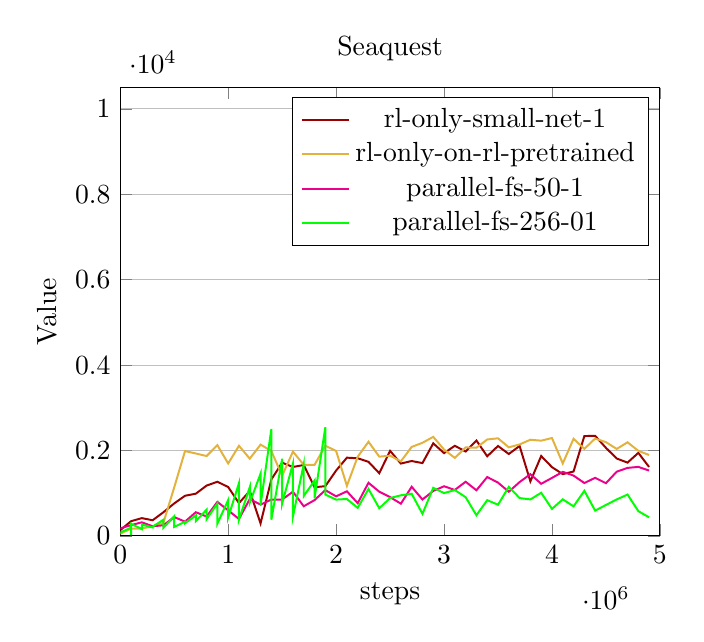
\begin{tikzpicture}

\begin{axis}[%
title=Seaquest,
% %width=4.634in,
%width=10in,
%height=5in,
%at={(2.596in,2.358in)},
% scale only axis,
xmin=0,
xmax=5000000,
xlabel style={font=\color{white!15!black}},
xlabel={steps},
xlabel near ticks,
ymin=0,
ymax=10500,
ylabel style={font=\color{white!15!black}},
ylabel={Value},
ylabel near ticks,
ymajorgrids,
% %scale=0.5,
%scale=0.4,
axis background/.style={fill=white},
%legend style={legend cell align=left, align=left, draw=white!15!black}
]
\addplot [color=red, line width = 0.25mm]
                table[row sep=crcr]{
                  0 134.0\\ 
100000 344.0\\ 
200000 416.0\\ 
300000 366.0\\ 
400000 554.0\\ 
500000 760.0\\ 
600000 940.0\\ 
700000 988.0\\ 
800000 1178.0\\ 
900000 1268.0\\ 
1000000 1144.0\\ 
1100000 768.0\\ 
1200000 1052.0\\ 
1300000 292.0\\ 
1400000 1322.0\\ 
1500000 1714.0\\ 
1600000 1614.0\\ 
1700000 1660.0\\ 
1800000 1140.0\\ 
1900000 1164.0\\ 
2000000 1530.0\\ 
2100000 1832.0\\ 
2200000 1818.0\\ 
2300000 1734.0\\ 
2400000 1468.0\\ 
2500000 1992.0\\ 
2600000 1694.0\\ 
2700000 1754.0\\ 
2800000 1704.0\\ 
2900000 2168.0\\ 
3000000 1938.0\\ 
3100000 2110.0\\ 
3200000 1976.0\\ 
3300000 2234.0\\ 
3400000 1864.0\\ 
3500000 2106.0\\ 
3600000 1918.0\\ 
3700000 2106.0\\ 
3800000 1276.0\\ 
3900000 1870.0\\ 
4000000 1610.0\\ 
4100000 1446.0\\ 
4200000 1508.0\\ 
4300000 2338.0\\ 
4400000 2344.0\\ 
4500000 2062.0\\ 
4600000 1812.0\\ 
4700000 1716.0\\ 
4800000 1944.0\\ 
4900000 1614.0\\ 
};
\addlegendentry{rl-only-small-net-1}
\addplot [color=yellow, line width = 0.25mm]
                table[row sep=crcr]{
                  0 48.0\\ 
100000 172.0\\ 
200000 172.0\\ 
300000 224.0\\ 
400000 308.0\\ 
500000 1136.0\\ 
600000 1986.0\\ 
700000 1930.0\\ 
800000 1870.0\\ 
900000 2124.0\\ 
1000000 1696.0\\ 
1100000 2110.0\\ 
1200000 1808.0\\ 
1300000 2138.0\\ 
1400000 1988.0\\ 
1500000 1408.0\\ 
1600000 1974.0\\ 
1700000 1664.0\\ 
1800000 1662.0\\ 
1900000 2112.0\\ 
2000000 1990.0\\ 
2100000 1172.0\\ 
2200000 1854.0\\ 
2300000 2204.0\\ 
2400000 1856.0\\ 
2500000 1878.0\\ 
2600000 1746.0\\ 
2700000 2084.0\\ 
2800000 2180.0\\ 
2900000 2320.0\\ 
3000000 2022.0\\ 
3100000 1826.0\\ 
3200000 2072.0\\ 
3300000 2064.0\\ 
3400000 2258.0\\ 
3500000 2286.0\\ 
3600000 2074.0\\ 
3700000 2142.0\\ 
3800000 2252.0\\ 
3900000 2230.0\\ 
4000000 2292.0\\ 
4100000 1696.0\\ 
4200000 2274.0\\ 
4300000 2038.0\\ 
4400000 2280.0\\ 
4500000 2196.0\\ 
4600000 2036.0\\ 
4700000 2192.0\\ 
4800000 1992.0\\ 
4900000 1894.0\\ 
};
\addlegendentry{rl-only-on-rl-pretrained}
\addplot [color=magenta, line width = 0.25mm]
                table[row sep=crcr]{
                  0 176.0\\ 
0 176.0\\ 
100000 252.0\\ 
200000 318.0\\ 
300000 226.0\\ 
400000 248.0\\ 
500000 440.0\\ 
600000 334.0\\ 
700000 554.0\\ 
800000 454.0\\ 
900000 796.0\\ 
1000000 598.0\\ 
1100000 396.0\\ 
1200000 862.0\\ 
1300000 732.0\\ 
1400000 850.0\\ 
1500000 852.0\\ 
1600000 1034.0\\ 
1700000 694.0\\ 
1800000 838.0\\ 
1900000 1072.0\\ 
2000000 926.0\\ 
2100000 1044.0\\ 
2200000 766.0\\ 
2300000 1244.0\\ 
2400000 1034.0\\ 
2500000 908.0\\ 
2600000 754.0\\ 
2700000 1150.0\\ 
2800000 852.0\\ 
2900000 1052.0\\ 
3000000 1162.0\\ 
3100000 1076.0\\ 
3200000 1268.0\\ 
3300000 1068.0\\ 
3400000 1378.0\\ 
3500000 1248.0\\ 
3600000 1034.0\\ 
3700000 1260.0\\ 
3800000 1446.0\\ 
3900000 1220.0\\ 
4000000 1358.0\\ 
4100000 1500.0\\ 
4200000 1412.0\\ 
4300000 1238.0\\ 
4400000 1360.0\\ 
4500000 1234.0\\ 
4600000 1504.0\\ 
4700000 1592.0\\ 
4800000 1616.0\\ 
4900000 1530.0\\ 
};
\addlegendentry{parallel-fs-50-1}
\addplot [color=green, line width = 0.25mm]
                table[row sep=crcr]{
                  0 80.0\\ 
0 80.0\\ 
0 80.0\\ 
100000 192.0\\ 
100000 20.0\\ 
100000 284.0\\ 
200000 158.0\\ 
200000 264.0\\ 
300000 198.0\\ 
300000 216.0\\ 
400000 378.0\\ 
400000 192.0\\ 
500000 460.0\\ 
500000 210.0\\ 
600000 330.0\\ 
600000 296.0\\ 
700000 478.0\\ 
700000 344.0\\ 
800000 614.0\\ 
800000 390.0\\ 
900000 758.0\\ 
900000 288.0\\ 
1000000 840.0\\ 
1000000 432.0\\ 
1100000 1236.0\\ 
1100000 384.0\\ 
1200000 1142.0\\ 
1200000 776.0\\ 
1300000 1458.0\\ 
1300000 730.0\\ 
1400000 2504.0\\ 
1400000 380.0\\ 
1500000 1806.0\\ 
1500000 756.0\\ 
1600000 1695.0\\ 
1600000 454.0\\ 
1700000 1678.0\\ 
1700000 932.0\\ 
1800000 1296.0\\ 
1800000 878.0\\ 
1900000 2544.0\\ 
1900000 968.0\\ 
2000000 850.0\\ 
2100000 864.0\\ 
2200000 656.0\\ 
2300000 1098.0\\ 
2400000 648.0\\ 
2500000 886.0\\ 
2600000 950.0\\ 
2700000 988.0\\ 
2800000 516.0\\ 
2900000 1126.0\\ 
3000000 1002.0\\ 
3100000 1074.0\\ 
3200000 906.0\\ 
3300000 484.0\\ 
3400000 836.0\\ 
3500000 730.0\\ 
3600000 1148.0\\ 
3700000 886.0\\ 
3800000 854.0\\ 
3900000 1010.0\\ 
4000000 632.0\\ 
4100000 856.0\\ 
4200000 692.0\\ 
4300000 1056.0\\ 
4400000 592.0\\ 
4500000 724.0\\ 
4600000 854.0\\ 
4700000 968.0\\ 
4800000 580.0\\ 
4900000 434.0\\ 
};
\addlegendentry{parallel-fs-256-01}
\end{axis}
\end{tikzpicture}}}\\
%  \vspace{-1cm}
%    \subfloat[]{  \resizebox{0.4\textwidth}{!}{
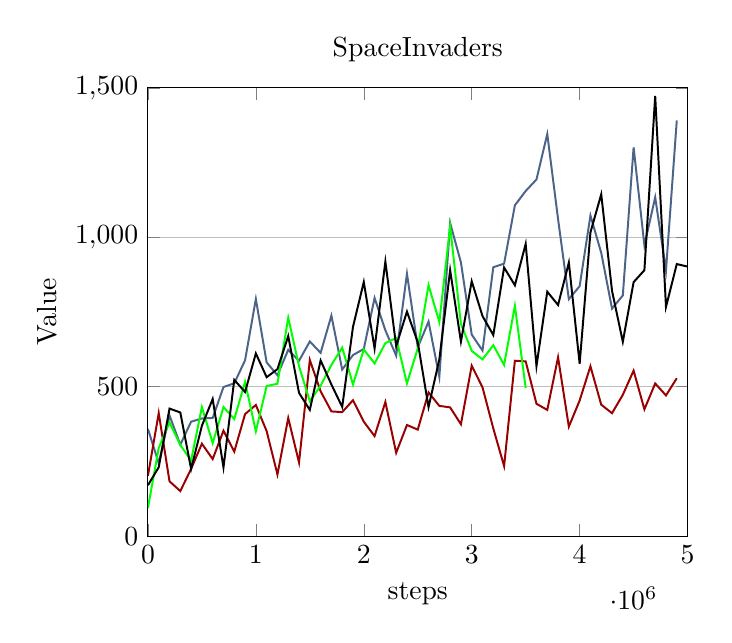
\begin{tikzpicture}

\begin{axis}[%
title=SpaceInvaders,
%width=10in,
%height=5in,
%at={(2.596in,2.358in)},
% scale only axis,
xmin=0,
xmax=5000000,
xlabel style={font=\color{white!15!black}},
xlabel={steps},
xlabel near ticks,
ymin=0,
ymax=1500,
ylabel style={font=\color{white!15!black}},
ylabel={Value},
ylabel near ticks,
ymajorgrids,
% %scale=0.5,
%scale=0.4,
axis background/.style={fill=white},
%legend style={legend cell align=left, align=left, draw=white!15!black}
]
\addplot [color=blue, line width = 0.25mm]
                table[row sep=crcr]{
                  0 359.0\\ 
100000 244.0\\ 
200000 404.0\\ 
300000 306.0\\ 
400000 383.0\\ 
500000 394.0\\ 
600000 395.5\\ 
700000 499.0\\ 
800000 511.5\\ 
900000 588.5\\ 
1000000 793.5\\ 
1100000 581.5\\ 
1200000 538.5\\ 
1300000 623.5\\ 
1400000 587.0\\ 
1500000 651.5\\ 
1600000 613.5\\ 
1700000 738.0\\ 
1800000 557.5\\ 
1900000 606.0\\ 
2000000 626.5\\ 
2100000 797.0\\ 
2200000 689.0\\ 
2300000 604.0\\ 
2400000 878.0\\ 
2500000 632.0\\ 
2600000 718.0\\ 
2700000 533.0\\ 
2800000 1048.0\\ 
2900000 916.0\\ 
3000000 674.5\\ 
3100000 621.0\\ 
3200000 900.0\\ 
3300000 912.0\\ 
3400000 1107.0\\ 
3500000 1155.0\\ 
3600000 1193.5\\ 
3700000 1345.5\\ 
3800000 1061.0\\ 
3900000 793.0\\ 
4000000 836.5\\ 
4100000 1073.0\\ 
4200000 948.0\\ 
4300000 761.5\\ 
4400000 805.5\\ 
4500000 1301.0\\ 
4600000 973.0\\ 
4700000 1134.0\\ 
4800000 889.5\\ 
4900000 1391.0\\ 
};
\addplot [color=red, line width = 0.25mm]
                table[row sep=crcr]{
                  0 202.0\\ 
100000 412.0\\ 
200000 183.5\\ 
300000 151.0\\ 
400000 225.0\\ 
500000 309.5\\ 
600000 258.0\\ 
700000 353.0\\ 
800000 283.0\\ 
900000 408.5\\ 
1000000 439.0\\ 
1100000 351.5\\ 
1200000 206.5\\ 
1300000 395.5\\ 
1400000 246.5\\ 
1500000 589.5\\ 
1600000 485.0\\ 
1700000 417.5\\ 
1800000 415.0\\ 
1900000 455.0\\ 
2000000 383.0\\ 
2100000 335.0\\ 
2200000 449.0\\ 
2300000 279.0\\ 
2400000 372.0\\ 
2500000 356.5\\ 
2600000 481.0\\ 
2700000 436.0\\ 
2800000 431.0\\ 
2900000 374.5\\ 
3000000 570.5\\ 
3100000 498.0\\ 
3200000 360.5\\ 
3300000 234.5\\ 
3400000 587.0\\ 
3500000 585.0\\ 
3600000 443.0\\ 
3700000 422.5\\ 
3800000 598.5\\ 
3900000 366.5\\ 
4000000 454.0\\ 
4100000 568.5\\ 
4200000 440.0\\ 
4300000 411.5\\ 
4400000 473.0\\ 
4500000 554.0\\ 
4600000 424.5\\ 
4700000 511.0\\ 
4800000 471.0\\ 
4900000 528.5\\ 
};
\addplot [color=green, line width = 0.25mm]
                table[row sep=crcr]{
                  0 94.5\\ 
100000 295.0\\ 
200000 380.5\\ 
300000 305.0\\ 
400000 253.0\\ 
500000 432.0\\ 
600000 311.5\\ 
700000 432.0\\ 
800000 392.0\\ 
900000 516.0\\ 
1000000 351.0\\ 
1100000 502.5\\ 
1200000 510.0\\ 
1300000 731.0\\ 
1400000 569.0\\ 
1500000 451.5\\ 
1600000 503.5\\ 
1700000 573.0\\ 
1800000 631.0\\ 
1900000 507.5\\ 
2000000 624.5\\ 
2100000 578.0\\ 
2200000 646.0\\ 
2300000 663.0\\ 
2400000 511.0\\ 
2500000 628.0\\ 
2600000 840.0\\ 
2700000 716.5\\ 
2800000 1037.0\\ 
2900000 710.5\\ 
3000000 620.0\\ 
3100000 591.5\\ 
3200000 639.0\\ 
3300000 573.0\\ 
3400000 771.0\\ 
3500000 496.0\\ 
};
\addplot [color=black, line width = 0.25mm]
                table[row sep=crcr]{
                  0 170.5\\ 
100000 230.5\\ 
200000 427.0\\ 
300000 414.0\\ 
400000 225.0\\ 
500000 369.5\\ 
600000 459.0\\ 
700000 230.0\\ 
800000 523.0\\ 
900000 482.5\\ 
1000000 611.5\\ 
1100000 532.0\\ 
1200000 559.0\\ 
1300000 669.5\\ 
1400000 479.5\\ 
1500000 422.5\\ 
1600000 588.0\\ 
1700000 507.5\\ 
1800000 432.5\\ 
1900000 700.5\\ 
2000000 850.5\\ 
2100000 628.0\\ 
2200000 919.0\\ 
2300000 636.0\\ 
2400000 751.5\\ 
2500000 649.0\\ 
2600000 432.0\\ 
2700000 591.5\\ 
2800000 890.0\\ 
2900000 651.0\\ 
3000000 853.0\\ 
3100000 736.5\\ 
3200000 673.0\\ 
3300000 899.0\\ 
3400000 839.5\\ 
3500000 978.0\\ 
3600000 569.0\\ 
3700000 818.0\\ 
3800000 773.5\\ 
3900000 915.5\\ 
4000000 577.0\\ 
4100000 1016.5\\ 
4200000 1144.0\\ 
4300000 821.0\\ 
4400000 650.5\\ 
4500000 850.0\\ 
4600000 890.0\\ 
4700000 1473.0\\ 
4800000 767.0\\ 
4900000 910.5\\ 
5000000 902.0\\ 
};
\end{axis}
\end{tikzpicture}}}
%  \\
%
%  \ref{named}
%  \caption{caption text 23}
%  \label{fig:compare}
%\end{figure}




\chapter{Discussion}
\label{ch-discussion}
%\section{}
Overall, the results are both disappointing and inconclusive.
%Having that said, there are some clear takeaways to guide further research.
Both intuitively and by being informed with the relevant literature,
we expected stronger results. 
In this section we explore possible explanations for the results
and use them to suggest promising avenues for further research.
We break our discussion of the results into answering the following questions:
\begin{enumerate}
		\item What are the differences between features and states 
				and how important are they to the final performance?
		\item Why is reconstruction loss particularly bad at representing
				stateful information?
		\item What could be the characteristics of more successful approaches
				to using unsupervised learning for state representation learning?
		\item What role does regularization play in reinforcement learning,
				unsupervised learning and their combination?
\end{enumerate}

Given the generality of our hypothesis, we of course can not answer these questions fully,
but we can give hints and suggestions.

\section{Differences between features and states}
We believe that the central idea behind using unsupervised representation learning
as state representation learning is the one illustrated in \ref{fig-rl-srl-features-space}.
If the hypothesis behind it is correct, then learning should be faster.
This is certainly the case in numerous works which use shared layers for actors 
and critics in actor-critic methods.
Of course, this only works on the condition that
the inherent instabilities in training networks with different losses have been taken care of 
in one way or another.
The specific differences between our features and states will be further discussed in
the following subsections, while a more general discussion will be held here.

When looking at simple games such as Pong or Seaquest,
one can clearly see what constitutes a state.
The dynamic information primarily consists of the positions and velocities of objects in the image.
More static information would be the types of objects, for example the player, projectiles, obstacles etc., 
and similar information.
For such simple problems, a resourceful engineering could easily craft representations consisting of at most
a few dozen parameters.
From our experiments with different autoencoder architectures and sets of hyperparameters,
we could not obtained such low-dimensional representations through unsupervised learning.
While deep learning experts could certainly tailor the various parameters and the training process
for each specific game and thereby obtain lower dimensionality, the point of finding
general purpose reinforcement learning solutions would be lost.
After all, one could (relatively) easily hand-craft near-perfect solutions for every
Atari57 game.
Thus we are left with the conclusion that even if unsupervised learning methods 
can help reinforcement learning, they by themselves are not the key to getting (super) human speed in
acquiring knowledge in control problems.

We therefore propose two avenues toward highly sample-efficient reinforcement learning.
One is to formulate model or state representation learning which is geared specifically toward learning dynamics
and to make it more restrictive. In other words to find more inspiration in works such as \cite{pilco}.
This way single problems can be quickly learned from scratch.
Another is quite the opposite and more inspired by humans. 
Humans generalize across all of their experiences, which is what enables them to 
quickly make sense of novel situations.
Similarly, very large neural network models could also leverage such broad
representations to learn quickly. 
An interesting start would be to see whether a single network could be trained to play most Atari games,
and other games as well and learn new games quicker than starting from scratch by leveraging
its implicit representations.

There is another important broad conclusion to be drawn from the gap between our expectations
and our results.
We expected the results to be better because our vague sense of what is a feature
learned through either unsupervised or reinforcement learning led us to believe that they are related.
This would probably not have happened if we had a better understanding of what these features really are.
Hence we believe that having tools to investigate the nature of features obtained through deep learning would help
tremendously in designing unsupervised learning techniques for state representation learning.
Thus better understanding and explainability of neural networks would help not only
in safety of systems relying on it, but also in algorithm design ---
just looking at the final result and other indirect metrics is not good enough.




\section{Reconstruction loss}
\label{sec-rec-loss-bad}
Using pixel-reconstruction loss in general, and MSE loss in particular is a very poor choice for state representation learning.
A good reconstruction contains plenty of non-stateful information, while a poor one
looses stateful information while still keeping a lot of non-stateful information.
The reason for this is that lowering pixel-reconstruction loss does not directly incentivize learning
about states.
We believed that simply lowering dimensionality would make the reinforcement learning problem easier,
but this is clearly not the case unless non-stateful information is removed.
Loosely speaking,
with encoders trained via pixel-reconstruction the entropy remains roughly the same
when seen through the lens of reinforcement learning.
As already mentioned, parallel training objectives make the training process more unstable
which hinders progress.
Hence the representation being learned needs to be good enough to overcome this negative effect
and better still in order to obtain tangible benefits.

Furthermore, having a generative model significantly increases the wall-clock training time (200-400\%)
due to the networks needing more parameters and due to the existence of the decoder.
For this reason discriminative models should be preferred for state representation learning
and as seen in \ref{ch-related-work} this is a clear trend in recent years.
Generative models still have their place in model-based approaches of course.



\section{Importance of representing dynamics}
Forward prediction in pixel-space showed an edge over just compression.
While theoretically sound, this is somewhat surprising given the fact that 
the reconstruction error was over a magnitude larger than in the case of just compression.
This clearly shows the importance of directly incentivizing learning stateful information.
There are numerous improvements which could be made to improve the quality of predictions:
\begin{itemize}
		\item learning to predict further into the future with the help of curriculum learning should
increase the accuracy on shorter time scale
\item more specialized architectures like using temporal-convolutions, having separate parameters 
		for each action in the decoder,...
\end{itemize}
We refrain from suggesting further improvements because as discussed in \ref{sec-rec-loss-bad},
we believe that reconstruction loss is a bad choice for state representation learning 
and that an all together different approach should be taken, ex. self-predictive bootstrapped latent
representations.


\section{Not all regularization is the same}
As shown in \ref{sec-effectiveness-of-reg}, improper regularization hurts learning, while
meaningful regularization helps.
In our context regularization serves to stabilize the learning process.
This mainly refers to preventing the latent representations to shift over time,
i.e. to produce the same latent representations when given the same frames.
Since L2 regularization constricts the manifold of latent representations,
it serves this purpose well.

In our implementation, data augmentation seems to only introduce noise because it makes
the encoder produce
different latent vectors when given the same frame.
Interestingly, it had a positive effect on learning in runs with 10 times more frequent
network updates (compared to environment steps), but as we performed these runs
on a limited number of games this claim can not be further corroborated with substantial evidence.

%\section{}
